\documentclass[11pt,a4paper,twoside,openany]{book}
% =====================================================================
% Preambuła książki naukowej wiernie wzorowana na „Mathematics for Machine
% Learning” (Deisenroth, Faisal, Ong):
%  - czcionka Times, czarno-biały skład, bez kolorowych ramek,
%  - definicje i twierdzenia: pogrubiony nagłówek w tekście, bez ramki,
%  - szare tło TYLKO dla przykładów,
%  - szeroki margines: podpisy rysunków, hasła (\haslo) i uwagi na marginesie,
%  - uwagi i intuicje jako kursywne „Uwaga.” zakończone znakiem ◊,
%  - nagłówek strony: numer + kursywny tytuł rozdziału / sekcji, bez linii.
% Wykresy powstają osobno w Pythonie (figures/) i wchodzą jako obrazy.
% =====================================================================
\usepackage[T1]{fontenc}
\usepackage[utf8]{inputenc}
\usepackage[polish]{babel}
\usepackage{mathptmx}              % Times + dopasowana matematyka
\usepackage{microtype}
\usepackage{amsmath,amssymb,amsthm,mathtools,bm}
\usepackage{booktabs,array}
\usepackage{graphicx}
\usepackage{xcolor}
\usepackage{enumitem}
\setlist[enumerate]{leftmargin=*,itemsep=2pt,topsep=3pt}
\setlist[itemize]{leftmargin=*,itemsep=2pt,topsep=3pt}

% ---------- układ strony: szeroki zewnętrzny margines ----------
\usepackage[a4paper,twoside,inner=2.4cm,textwidth=11.6cm,marginparsep=0.55cm,
  marginparwidth=4.9cm,top=2.7cm,bottom=2.9cm,headheight=14pt,headsep=0.9cm]{geometry}
\usepackage{sidenotes}             % \sidenote, \sidecaption, marginfigure, figure*
\definecolor{mmlgray}{gray}{0.94}  % jedyny „kolor” książki: szare tło przykładów

\usepackage{hyperref}
\hypersetup{colorlinks=true,linkcolor=black,citecolor=black,urlcolor=black,
  pdfauthor={},pdftitle={}}
\usepackage{cleveref}
\crefname{figure}{rys.}{rys.}\Crefname{figure}{Rysunek}{Rysunki}
\crefname{table}{tab.}{tab.}\Crefname{table}{Tabela}{Tabele}
\crefname{equation}{wzór}{wzory}\Crefname{equation}{Wzór}{Wzory}
\crefname{chapter}{rozdział}{rozdziały}\Crefname{chapter}{Rozdział}{Rozdziały}
\crefname{section}{sekcja}{sekcje}\Crefname{section}{Sekcja}{Sekcje}
\crefname{definicja}{def.}{def.}\Crefname{definicja}{Definicja}{Definicje}
\crefname{twierdzenie}{tw.}{tw.}\Crefname{twierdzenie}{Twierdzenie}{Twierdzenia}
\crefname{lemat}{lemat}{lematy}\Crefname{lemat}{Lemat}{Lematy}
\crefname{wniosek}{wniosek}{wnioski}\Crefname{wniosek}{Wniosek}{Wnioski}
\crefname{przyklad}{przykład}{przykłady}\Crefname{przyklad}{Przykład}{Przykłady}

\numberwithin{equation}{chapter}   % (2.94): numer rozdziału i wzoru

% ---------- nagłówki rozdziałów i sekcji (jak w MML: czarne, pogrubione) ----------
\usepackage[explicit]{titlesec}
\titleformat{\chapter}[hang]{\bfseries\fontsize{26}{30}\selectfont}{\thechapter}{0.9em}{#1}
\titleformat{name=\chapter,numberless}[hang]{\bfseries\fontsize{26}{30}\selectfont}{}{0pt}{#1}
\titlespacing*{\chapter}{0pt}{16pt}{34pt}
\titleformat{\section}{\large\bfseries}{\thesection}{0.8em}{#1}
\titleformat{\subsection}{\bfseries\itshape}{\thesubsection}{0.8em}{#1}
\titleformat{\paragraph}[runin]{\bfseries\itshape}{}{0pt}{#1.}
\titlespacing*{\section}{0pt}{2.8ex plus 1ex minus .2ex}{1.2ex plus .2ex}
\titlespacing*{\subsection}{0pt}{2.4ex plus 1ex minus .2ex}{1ex plus .2ex}

% ---------- nagłówki i stopki stron (numer + kursywny tytuł, bez linii) ----------
\usepackage{fancyhdr}
\pagestyle{fancy}
\fancyhf{}
\renewcommand{\headrulewidth}{0pt}
\renewcommand{\chaptermark}[1]{\markboth{#1}{}}
\renewcommand{\sectionmark}[1]{\markright{\thesection\ #1}}
\fancyhead[LE]{\thepage}
\fancyhead[RE]{\textit{\leftmark}}
\fancyhead[LO]{\textit{\rightmark}}
\fancyhead[RO]{\thepage}
\fancypagestyle{plain}{\fancyhf{}\fancyfoot[C]{\thepage}\renewcommand{\headrulewidth}{0pt}}

% ---------- spis treści: pogrubione rozdziały, bez kropek ----------
\usepackage{tocloft}
\renewcommand{\cfttoctitlefont}{\bfseries\fontsize{26}{30}\selectfont}
\renewcommand{\cftaftertoctitleskip}{24pt}
\renewcommand{\cftchapfont}{\bfseries}
\renewcommand{\cftchappagefont}{\bfseries}
\renewcommand{\cftdotsep}{\cftnodots}

% ---------- podpisy rysunków: mała czcionka, pogrubiona etykieta, w marginesie ----------
\captionsetup{font=footnotesize,labelfont=bf,justification=raggedright,
  singlelinecheck=off,skip=4pt}

% ---------- twierdzenia, definicje, przykłady ----------
\usepackage[most]{tcolorbox}
% nagłówek pogrubiony w tekście, bez ramki: „Definicja 2.10 (Nazwa).”
\newtheoremstyle{mmldef}{9pt}{9pt}{\normalfont}{0pt}{\bfseries}{.}{0.5em}
  {\thmname{#1}\ \thmnumber{#2}\thmnote{\ (#3)}}
\newtheoremstyle{mmlthm}{9pt}{9pt}{\itshape}{0pt}{\bfseries}{.}{0.5em}
  {\thmname{#1}\ \thmnumber{#2}\thmnote{\ (#3)}}
\theoremstyle{mmldef}
\newtheorem{definicja}{Definicja}[chapter]
\newtheorem{przyklad}{Przykład}[chapter]       % własna numeracja, jak w MML
\theoremstyle{mmlthm}
\newtheorem{twierdzenie}[definicja]{Twierdzenie}
\newtheorem{lemat}[definicja]{Lemat}
\newtheorem{wniosek}[definicja]{Wniosek}
\renewcommand{\qedsymbol}{$\blacksquare$}

% jedyna ramka: szare tło przykładów
\tcbset{mmlbox/.style={enhanced,breakable,sharp corners,frame hidden,boxrule=0pt,
  colback=mmlgray,left=8pt,right=8pt,top=5pt,bottom=5pt,
  before skip=11pt,after skip=11pt,before upper={\parindent0pt}}}
\tcolorboxenvironment{przyklad}{mmlbox}
\newtcolorbox{naliczbach}{mmlbox,
  before upper={\parindent0pt\textbf{Na konkretnych liczbach.}\ }}

% uwagi jak w MML: kursywna etykieta w tekście i znak ◊ na końcu
\newenvironment{mmluwaga}[1]{\par\smallskip\noindent\textit{#1.}\ }{\hfill$\diamondsuit$\par\smallskip}
\newenvironment{uwaga}{\begin{mmluwaga}{Uwaga}}{\end{mmluwaga}}
\newenvironment{intuicja}{\begin{mmluwaga}{Intuicja}}{\end{mmluwaga}}
\newenvironment{pulapka}{\begin{mmluwaga}{Pułapka}}{\end{mmluwaga}}
\newenvironment{pomyslDowodu}{\par\smallskip\noindent\textit{Pomysł dowodu.}\ }{\par\smallskip}

% ćwiczenia na końcu rozdziału: zwykła sekcja z listą
\newenvironment{sprawdz}{\subsection*{Ćwiczenia}}{}

% hasło w marginesie (jak terminy w MML): \haslo{wyznacznik}
\newcommand{\haslo}[1]{\marginnote{\footnotesize\raggedright #1}}

% Odesłanie do dowodu w dodatku (dla dowodów zbyt długich na rozdział).
\newcommand{\dowodw}[1]{\par\noindent\textit{Dowód: patrz \cref{#1}.}\par}

% ---------- skróty matematyczne (wektory pogrubione kursywą jak w MML) ----------
\let\Im\relax % w LaTeX-u \Im to część urojona; tu znaczy obraz przekształcenia
\DeclareMathOperator{\Im}{Im}
\DeclareMathOperator{\rk}{rk}
\DeclareMathOperator{\Ker}{Ker}
\DeclareMathOperator{\tr}{tr}
\DeclareMathOperator{\spn}{span}
\DeclareMathOperator*{\argmin}{arg\,min}
\DeclareMathOperator*{\argmax}{arg\,max}
\newcommand{\R}{\mathbb{R}}
\newcommand{\C}{\mathbb{C}}
\newcommand{\N}{\mathbb{N}}
\newcommand{\vect}[1]{\bm{#1}}
\newcommand{\norm}[1]{\left\lVert #1\right\rVert}
\newcommand{\ip}[2]{\left\langle #1,#2\right\rangle}
\newcommand{\abs}[1]{\left\lvert #1\right\rvert}

% ---------- schematy w TikZ (tylko proste diagramy; wykresy robimy w Pythonie) ----------
\usepackage{tikz}
\usetikzlibrary{arrows.meta,calc,positioning,shapes.geometric,fit,backgrounds}
\tikzset{
  wektor/.style={-{Stealth[length=2.2mm]},thick},
  pomocnicza/.style={dashed,gray},
  wezel/.style={circle,draw,thick,minimum size=7mm,inner sep=1pt},
  blok/.style={rectangle,draw,thick,minimum height=8mm,minimum width=18mm,align=center,fill=white}
}

% ---------- strona tytułowa (czarno-biała) ----------
% \tytulksiazki{Tytuł}{Podtytuł}{Autor}
\newcommand{\tytulksiazki}[3]{%
  \begin{titlepage}
  \thispagestyle{empty}
  \vspace*{4.5cm}
  {\raggedright\bfseries\fontsize{40}{46}\selectfont #1\par}
  \vspace{1.0cm}
  {\raggedright\Large #2\par}
  \vfill
  {\raggedright\Large #3\par}
  \vspace{1.5cm}
  \end{titlepage}}

% ---------- makra tej książki (model Gen 6) ----------
\DeclareMathOperator{\softmax}{softmax}
\DeclareMathOperator{\GELU}{GELU}
\DeclareMathOperator{\LN}{LN}
\DeclareMathOperator{\Drop}{Drop}
\DeclareMathOperator{\MLP}{MLP}
\DeclareMathOperator{\Conv}{Conv}
\DeclareMathOperator{\DW}{DW}
\DeclareMathOperator{\shift}{shift}
\DeclareMathOperator{\clip}{clip}
\DeclareMathOperator{\round}{round}
\DeclareMathOperator{\ReLU}{ReLU}
\DeclareMathOperator{\Var}{Var}
\DeclareMathOperator{\Exp}{\mathbb{E}}
\DeclareMathOperator{\sg}{sg}
\newcommand{\indic}[1]{\mathbb{1}\!\left[#1\right]}
\newcommand{\ie}{tzn.\ }
\newcommand{\kodlink}[1]{\texttt{#1}}
\newcommand{\Hz}{\,\mathrm{Hz}}
\newcommand{\dB}{\,\mathrm{dB}}
\newcommand{\ms}{\,\mathrm{ms}}
\newcommand{\pow}[1]{\text{\footnotesize #1}}   % krótka adnotacja przy kroku dowodu


\begin{document}
\frontmatter
\tytulksiazki{Jak słyszy Gen 6}{Matematyka od zera i model transkrypcji gitary: od fali dźwiękowej do listy nut}{Projekt Gutar}
\tableofcontents

\mainmatter
\chapter{Zapis, tensory i logarytm}\label{rozdz:zapis}

\section{Po co ten rozdział?}

Model, któremu poświęcona jest ta książka, bierze nagranie gitary i zwraca listę nut. W środku
nie dzieje się nic magicznego: to ciąg operacji na tablicach liczb. Zanim opiszemy te operacje,
musimy się umówić, jak zapisywać tablice, sumy i funkcje. Ten rozdział jest krótką umową
o języku. Kto zna sumy, indeksy i logarytmy, może go przejrzeć i przejść do rozdziału~\ref{rozdz:dzwiek};
wszystko, co tu zdefiniujemy, jest używane do końca książki.

Po tym rozdziale umiesz: (i)~odczytać kształt tensora i policzyć, ile ma liczb, (ii)~zapisać
złożenie funkcji jako ciąg kroków, (iii)~uzasadnić, dlaczego logarytm zamienia mnożenie na dodawanie.

\section{Sumy i indeksy}

\haslo{suma}
\begin{definicja}[Suma]\label{def:suma}
Dla liczb $a_1,a_2,\dots,a_n$ zapis
\begin{equation}
  \sum_{i=1}^{n} a_i \;=\; a_1+a_2+\dots+a_n
\end{equation}
oznacza ich sumę. Literę $i$ nazywamy \emph{indeksem}; może być dowolna, bo znika po rozpisaniu sumy.
Gdy $n=0$, suma jest pusta i wynosi $0$.
\end{definicja}

\begin{przyklad}\label{prz:suma}
$\sum_{i=1}^{4} i^2 = 1+4+9+16 = 30$. Ta sama suma zapisana z indeksem $k$ od $0$ do $3$ wygląda
$\sum_{k=0}^{3}(k+1)^2$ i też daje $30$. Zmiana nazwy indeksu ani jego zakresu (z odpowiednim
przesunięciem we wzorze) nie zmienia wyniku.
\end{przyklad}

\begin{intuicja}
Znak $\sum$ to pętla \texttt{for}, która dodaje: \texttt{s=0; for i in range(1,n+1): s+=a[i]}.
W kodzie indeksy zaczynają się od $0$, w matematyce od $1$; w tej książce zawsze powiemy, od czego.
\end{intuicja}

Sumy będą nam potrzebne wszędzie: iloczyn skalarny to suma iloczynów, średnia to suma podzielona
przez liczbę elementów, a strata modelu to średnia po tysiącach klatek.

\begin{twierdzenie}[Liniowość sumy]\label{tw:liniowosc-sumy}
Dla dowolnych liczb $a_i,b_i$ i stałej $c$ zachodzi
\begin{equation}
  \sum_{i=1}^{n}(c\,a_i+b_i)=c\sum_{i=1}^{n}a_i+\sum_{i=1}^{n}b_i .
\end{equation}
\end{twierdzenie}
\begin{pomyslDowodu}
Rozpisujemy sumę na składniki i korzystamy z przemienności oraz rozdzielności dodawania.
\end{pomyslDowodu}
\begin{proof}
\begin{align*}
\sum_{i=1}^{n}(c\,a_i+b_i)
 &= (c\,a_1+b_1)+(c\,a_2+b_2)+\dots+(c\,a_n+b_n)
   && \pow{(def.~sumy)}\\
 &= (c\,a_1+\dots+c\,a_n)+(b_1+\dots+b_n)
   && \pow{(zmiana kolejności)}\\
 &= c\,(a_1+\dots+a_n)+(b_1+\dots+b_n)
   && \pow{(rozdzielność)}\\
 &= c\sum_{i=1}^{n}a_i+\sum_{i=1}^{n}b_i .
   && \pow{(def.~sumy)}
\end{align*}
Każdy krok zmienia tylko zapis albo kolejność dodawania, więc równość zachodzi.
\end{proof}

W zwykłym języku: stałą wolno wyciągnąć przed sumę, a sumę sum wolno rozbić. Użyjemy tego, gdy będziemy
liczyć pochodną straty (rozdział~\ref{rozdz:pochodne}).

\section{Wektory, macierze i tensory}

\haslo{tensor}
\begin{definicja}[Tensor i jego kształt]\label{def:tensor}
\emph{Tensorem} nazywamy tablicę liczb rzeczywistych indeksowaną jedną lub kilkoma liczbami całkowitymi.
Liczba indeksów to \emph{rząd} tensora. Ciąg długości zakresów indeksów to \emph{kształt}.
Tensor rzędu $1$ to \emph{wektor}, rzędu $2$ to \emph{macierz}. Zapis $X\in\R^{n_1\times n_2\times\dots\times n_r}$
oznacza tensor kształtu $(n_1,\dots,n_r)$; ma on $n_1 n_2\cdots n_r$ liczb.
\end{definicja}

\begin{przyklad}[Cechy jednego nagrania]\label{prz:tensor-hcqt}
Model Gen~6 zamienia nagranie na tensor $X\in\R^{T\times 9\times 159}$ (rozdział~\ref{rozdz:hcqt}): $T$
klatek czasu, $9$ kanałów i $159$ binów częstotliwości. Nagranie trwające 6 sekund daje $T=243$ klatek,
więc $X$ ma $243\cdot 9\cdot 159=347\,733$ liczb. Element $X_{t,c,p}$ to liczba z klatki $t$,
kanału $c$ i binu $p$.
\end{przyklad}

\begin{figure}[ht]
\centering
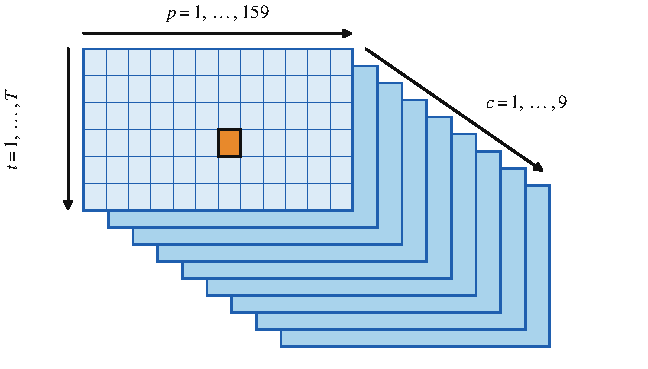
\includegraphics[width=\linewidth]{figures/tensor.pdf}
\sidecaption{Tensor $X\in\R^{T\times9\times159}$ jako stos dziewięciu macierzy (kanałów); przedni płat ($c=1$) ma narysowaną siatkę: $T$ wierszy (oś $t$, w dół) i $159$ kolumn (oś $p$, poziomo), a kolejne kanały leżą za nim (oś $c$).
Pomarańczowa kratka to jeden element $X_{t,c,p}$; trzy indeksy jednoznacznie wskazują jedną liczbę. \label{rys:tensor}}
\end{figure}

\begin{pulapka}
Kształt $(T,C,P)$ i kształt $(C,T,P)$ to dwa różne tensory, nawet gdy mają tyle samo liczb. W kodzie PyTorch
sieć dostaje tensor $[B,C,T,P]$ (paczka, kanały, czas, biny), a cechy zapisujemy jako $[T,C,P]$. Zawsze
sprawdzaj kształt przed operacją; błąd w kolejności osi daje poprawnie działający program z bezsensownym wynikiem.
\end{pulapka}

\section{Funkcje i ich składanie}

\haslo{złożenie funkcji}
\begin{definicja}[Funkcja i złożenie]\label{def:zlozenie}
\emph{Funkcja} $f\colon A\to B$ przypisuje każdemu elementowi zbioru $A$ dokładnie jeden element zbioru $B$.
\emph{Złożeniem} funkcji $f\colon A\to B$ i $g\colon B\to C$ jest funkcja $g\circ f\colon A\to C$,
$(g\circ f)(x)=g(f(x))$.
\end{definicja}

\begin{przyklad}\label{prz:zlozenie}
Niech $f(x)=2x$ i $g(x)=x+3$. Wtedy $(g\circ f)(5)=g(10)=13$, a $(f\circ g)(5)=f(8)=16$. Kolejność ma znaczenie:
złożenie nie jest przemienne.
\end{przyklad}

\begin{intuicja}
Cały model Gen~6 to jedno długie złożenie $\mathrm{model}=f_n\circ\dots\circ f_2\circ f_1$: cechy wchodzą do
pierwszej warstwy, jej wynik do drugiej itd. W rozdziale~\ref{rozdz:opis} rozpiszemy je w całości.
Dlatego ważne jest, by każda warstwa miała jasno określone wejście i wyjście: ich kształty muszą do siebie pasować.
\end{intuicja}

\begin{figure}[ht]
\centering
\begin{tikzpicture}[>=Stealth,node distance=0.85cm,blok/.append style={minimum width=12mm}]
  \node[blok] (x) {$\vect x$};
  \node[blok,right=of x] (f1) {$f_1$};
  \node[blok,right=of f1] (f2) {$f_2$};
  \node[blok,right=of f2] (f3) {$f_3$};
  \node[blok,right=of f3] (y) {$\vect y$};
  \draw[wektor] (x)--(f1); \draw[wektor] (f1)--(f2); \draw[wektor] (f2)--(f3); \draw[wektor] (f3)--(y);
  \node[font=\footnotesize,above=0.5mm of $(x.east)!0.5!(f1.west)$] {$\R^{n_0}$};
  \node[font=\footnotesize,above=0.5mm of $(f1.east)!0.5!(f2.west)$] {$\R^{n_1}$};
  \node[font=\footnotesize,above=0.5mm of $(f2.east)!0.5!(f3.west)$] {$\R^{n_2}$};
  \node[font=\footnotesize,above=0.5mm of $(f3.east)!0.5!(y.west)$] {$\R^{n_3}$};
\end{tikzpicture}
\sidecaption{Złożenie trzech funkcji $\vect y=f_3(f_2(f_1(\vect x)))$. Nad strzałkami stoją przestrzenie, w których
żyje wynik każdego kroku; wyjście jednej funkcji musi mieć kształt wejścia następnej. \label{rys:zlozenie}}
\end{figure}

\section{Potęgi i logarytm}

Wysokość dźwięku, głośność w decybelach i położenie binu na osi częstotliwości są w tej książce mierzone
\emph{logarytmicznie}. Powód zobaczymy w rozdziale~\ref{rozdz:dzwiek}; tu przypominamy narzędzie.

\haslo{logarytm}
\begin{definicja}[Logarytm]\label{def:log}
Dla $b>0$, $b\neq1$ i $x>0$ \emph{logarytmem} $\log_b x$ nazywamy jedyną liczbę $y$, dla której $b^{y}=x$.
Logarytm przy podstawie $e$ oznaczamy $\ln x$, a przy podstawie $10$ po prostu $\log_{10}x$.
\end{definicja}

\begin{przyklad}\label{prz:log}
$\log_2 8=3$, bo $2^3=8$. $\log_2\tfrac12=-1$, bo $2^{-1}=\tfrac12$. $\log_2 3\approx1{,}585$, bo
$2^{1{,}585}\approx3$. Logarytmu z liczby niedodatniej nie ma, bo żadna potęga liczby dodatniej nie jest
ujemna ani zerowa.
\end{przyklad}

\begin{twierdzenie}[Logarytm iloczynu]\label{tw:log-iloczynu}
Dla $x,y>0$ zachodzi $\log_b(xy)=\log_b x+\log_b y$ oraz $\log_b(x^{k})=k\log_b x$ dla każdej liczby rzeczywistej $k$.
\end{twierdzenie}
\begin{pomyslDowodu}
Zamieniamy $x$ i $y$ na potęgi podstawy $b$ i dodajemy wykładniki.
\end{pomyslDowodu}
\begin{proof}
Niech $u=\log_b x$ i $v=\log_b y$, czyli $x=b^{u}$ i $y=b^{v}$. Wtedy
\begin{align*}
xy &= b^{u}b^{v}=b^{u+v} && \pow{(wykładniki się dodają)}\\
\log_b(xy) &= u+v=\log_b x+\log_b y && \pow{(def.~\ref{def:log})}
\end{align*}
Dla potęgi: $x^{k}=(b^{u})^{k}=b^{uk}$, więc $\log_b(x^{k})=uk=k\log_b x$.
\end{proof}

Zdanie ludzkim językiem: logarytm zamienia \emph{mnożenie} na \emph{dodawanie}. Mnożenie częstotliwości
przez $2$ (oktawa wyżej) staje się dodaniem stałej $1$ do $\log_2 f$, bez względu na to, od jakiej
częstotliwości zaczynamy (\cref{rys:os-log}b). To jest sedno całej książki.

\begin{figure*}[ht]
\centering
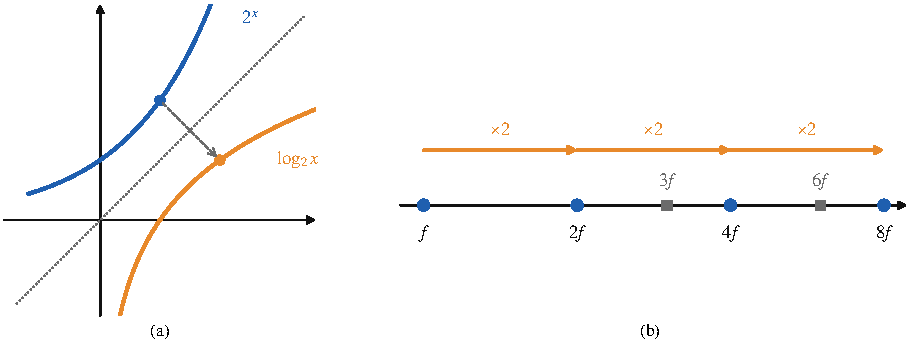
\includegraphics[width=\linewidth]{figures/os-log.pdf}
\caption{(a) Funkcje $2^x$ (niebieska) i $\log_2 x$ (pomarańczowa) są swoimi lustrzanymi odbiciami względem
prostej $y=x$ (kropkowana): odbicie punktu $(2,4)$ to $(4,2)$. (b) Na osi logarytmicznej kolejne podwojenia
$f,2f,4f,8f$ leżą w równych odstępach (pomarańczowe strzałki mają tę samą długość); punkty $3f$ i $6f$ też
dzieli dokładnie jeden taki krok, bo $\log_2 6-\log_2 3=1$.}
\label{rys:os-log}
\end{figure*}

\begin{naliczbach}
Ile wynosi $\log_2 12$? Zapisujemy $12=3\cdot 2^2$ i stosujemy twierdzenie~\ref{tw:log-iloczynu}:
$\log_2 12=\log_2 3+2\log_2 2=1{,}585+2=3{,}585$. Sprawdzenie: $2^{3{,}585}\approx 12{,}0$.
Ta sztuczka (rozbicie na iloczyn znanych czynników) pozwoli nam w rozdziale~\ref{rozdz:alikwoty} policzyć, ile półtonów
leży nad daną nutą jej trzeci alikwot.
\end{naliczbach}

\begin{twierdzenie}[Zmiana podstawy]\label{tw:zmiana-podstawy}
Dla $a,b>0$, $a,b\neq1$ i $x>0$ zachodzi $\log_b x=\dfrac{\log_a x}{\log_a b}$.
\end{twierdzenie}
\begin{pomyslDowodu}
Logarytmujemy obie strony równości $x=b^{\log_b x}$ przy podstawie $a$.
\end{pomyslDowodu}
\begin{proof}
Niech $y=\log_b x$, czyli $x=b^{y}$. Stosujemy $\log_a$ do obu stron:
\begin{align*}
\log_a x &= \log_a\!\big(b^{y}\big) && \pow{(podstawienie)}\\
         &= y\,\log_a b && \pow{(tw.~\ref{tw:log-iloczynu})}\\
\Rightarrow\; y &= \frac{\log_a x}{\log_a b}. && \pow{(dzielimy przez $\log_a b\neq0$)}
\end{align*}
Ponieważ $y=\log_b x$, to jest dokładnie dowodzony wzór.
\end{proof}

W praktyce: kalkulator ma zwykle tylko $\ln$ i $\log_{10}$, więc $\log_2 x=\ln x/\ln 2$. W programie \texttt{np.log2(x)}
daje to samo.

\section{Funkcje pomocnicze}

W modelu pojawi się kilka prostych funkcji, które warto poznać od razu.

\begin{figure*}[ht]
\centering
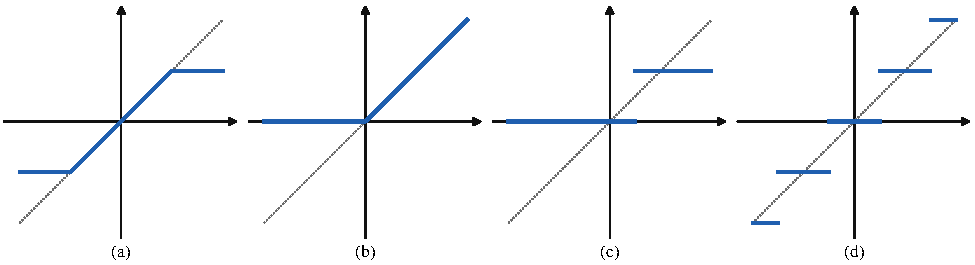
\includegraphics[width=\linewidth]{figures/funkcje-pomocnicze.pdf}
\caption{Cztery proste funkcje jednej zmiennej na tle prostej $y=x$ (kropkowana). (a) $\clip(x,-1,1)$ przycina wartości do przedziału.
(b) $\max(0,x)$, czyli $\ReLU$, zeruje wartości ujemne. (c) Wskaźnik $\indic{x\ge\frac12}$ jest równy $1$ albo $0$. (d) $\round(x)$ zaokrągla do najbliższej całkowitej.
Funkcje (c) i (d) mają skoki, więc nie da się ich używać w uczeniu przez gradient; dlatego dekoder w rozdziale~\ref{rozdz:dekoder} jest poza siecią.}
\label{rys:funkcje-pomocnicze}
\end{figure*}

\begin{center}\small
\begin{tabular}{@{}p{2.6cm}p{4.4cm}p{3.9cm}@{}}
\toprule
zapis & znaczenie & przykład\\
\midrule
$\clip(x,a,b)$ & $\min(\max(x,a),b)$ & $\clip(1{,}7;0;1{,}3)=1{,}3$\\
$\max_i a_i$ & największa z liczb & $\max(2,5,3)=5$\\
$\argmax_i a_i$ & \emph{numer} największej & $\argmax(2,5,3)=2$ (od 1)\\
$\indic{\text{warunek}}$ & $1$, gdy prawda, inaczej $0$ & $\indic{3>2}=1$\\
$\round(x)$ & najbliższa całkowita & $\round(35{,}07)=35$\\
$\lfloor x\rfloor$ & część całkowita w dół & $\lfloor 2{,}9\rfloor=2$\\
\bottomrule
\end{tabular}
\end{center}

\begin{pulapka}
$\argmax$ zwraca \emph{miejsce}, a $\max$ \emph{wartość}. Pomylenie ich jest tak częste, że w kodzie dekodera
(rozdział~\ref{rozdz:dekoder}) wybór struny to $\argmax$ po strunach, a pewność nuty to $\max$.
\end{pulapka}

\section*{Podsumowanie}
\begin{itemize}
\item Suma $\sum$ to pętla dodająca; stałą wolno wyciągnąć przed sumę (tw.~\ref{tw:liniowosc-sumy}).
\item Tensor to tablica liczb o kształcie $(n_1,\dots,n_r)$; cechy modelu to $X\in\R^{T\times9\times159}$.
\item Model to złożenie funkcji; kształty wyjść i wejść muszą do siebie pasować.
\item Logarytm zamienia mnożenie na dodawanie, a podwojenie częstotliwości na stały krok (tw.~\ref{tw:log-iloczynu}).
\item $\clip$, $\max$, $\argmax$, wskaźnik i zaokrąglenie to cegiełki dekodera i normalizacji cech.
\end{itemize}

\begin{sprawdz}
\begin{enumerate}
\item Policz $\sum_{i=1}^{5}(2i-1)$ i podaj wynik w prostszej postaci. (Wskazówka: tw.~\ref{tw:liniowosc-sumy} oraz $\sum i = n(n+1)/2$.)
\item Ile liczb ma tensor kształtu $[16,\,9,\,192,\,159]$ (paczka 16 wycinków po 192 klatki)? Ile to megabajtów w formacie \texttt{float16} (2 bajty na liczbę)?
\item Policz $\log_2 48$ i $\log_2\sqrt2$ bez kalkulatora, znając $\log_2 3\approx1{,}585$.
\item Czy $\log_b(x+y)=\log_b x+\log_b y$? Podaj kontrprzykład liczbowy.
\end{enumerate}
\end{sprawdz}

\subsection*{Rozwiązania}
\begin{enumerate}
\item $\sum_{i=1}^5(2i-1)=2\cdot15-5=25$ (suma pierwszych $n$ nieparzystych to $n^2$); sprawdzenie: $1+3+5+7+9=25$.
\item $16\cdot9\cdot192\cdot159=4\,396\,032$ liczb, czyli $\approx 8{,}8$~MB w \texttt{float16}.
\item $48=3\cdot2^4$, więc $\log_2 48=1{,}585+4=5{,}585$; $\log_2\sqrt2=\tfrac12$.
\item Nie. Dla $b=2$ i $x=y=4$ mamy $\log_2(4+4)=\log_2 8=3$, a $\log_2 4+\log_2 4=2+2=4$. Prawdziwy jest wzór na \emph{iloczyn}: $\log_2(4\cdot4)=\log_2 16=4$.
\end{enumerate}

\chapter{Dźwięk, próbkowanie i wysokość}\label{rozdz:dzwiek}

\section{Od drgania do liczb}

Struna gitary drga, pudło przekazuje drgania powietrzu, mikrofon zamienia zmiany ciśnienia na napięcie,
a komputer zapisuje to napięcie jako ciąg liczb. Cała wiedza, jaką model ma o nagraniu, to ten ciąg liczb.
Żeby ją wydobyć, trzeba najpierw zrozumieć dwie rzeczy: czym jest wysokość dźwięku
i co się traci przy zamianie fali ciągłej na liczby.

Po tym rozdziale umiesz: (i)~policzyć częstotliwość dowolnej nuty z jej numeru MIDI, (ii)~zmierzyć odstęp
dwóch dźwięków w centach, (iii)~uzasadnić, dlaczego model pracuje przy $11\,025\Hz$ i nie widzi wyższych częstotliwości
niż $5512{,}5\Hz$, (iv)~policzyć, ile klatek ma nagranie.

\section{Sinusoida}

\haslo{częstotliwość}
\begin{definicja}[Sinusoida, częstotliwość, okres]\label{def:sinusoida}
\emph{Sinusoidą} nazywamy sygnał $x(t)=A\sin(2\pi f t+\varphi)$ zmiennej $t$ (czas w sekundach). Liczba $A\ge0$ to
\emph{amplituda}, $f$ to \emph{częstotliwość} w hercach ($1\Hz$ = jeden pełny obieg na sekundę), a $\varphi$ to
\emph{faza}. Sygnał powtarza się co $T=1/f$ sekund; $T$ nazywamy \emph{okresem}.
\end{definicja}

\begin{przyklad}\label{prz:a4}
Strojowe A (nuta A4) ma $f=440\Hz$, więc okres $T=1/440\approx2{,}27\ms$. W ciągu jednej sekundy
powietrze wykonuje $440$ pełnych drgań. Dla sinusoidy $x(t)=0{,}5\sin(2\pi\cdot440\,t)$ największe wychylenie
wynosi $0{,}5$ i powtarza się co $2{,}27\ms$.
\end{przyklad}

\begin{intuicja}
Sinusoida to ruch punktu po okręgu oglądany z boku: faza mówi, skąd zaczynamy, a częstotliwość, ile obiegów
robimy na sekundę. Każdy dźwięk muzyczny to suma sinusoid; w rozdziale~\ref{rozdz:alikwoty} zobaczymy, że nuta gitary to
sinusoida $f_0$ i jej całkowite wielokrotności.
\end{intuicja}

\section{Próbkowanie}

Komputer nie widzi sygnału w każdej chwili, tylko co ułamek sekundy.

\haslo{próbkowanie}
\begin{definicja}[Próbkowanie]\label{def:probkowanie}
Dla sygnału $x(t)$ i \emph{częstotliwości próbkowania} $f_s$ ciąg próbek to $x[n]=x(n/f_s)$ dla $n=0,1,2,\dots$.
Jedna próbka to jedna liczba; nagranie trwające $\tau$ sekund ma $N=\tau f_s$ próbek.
\end{definicja}

\begin{przyklad}\label{prz:probkowanie}
Płyta CD ma $f_s=44\,100\Hz$, więc minuta dźwięku to $60\cdot 44\,100=2\,646\,000$ liczb. Model Gen~6 zmienia
próbkowanie nagrania na $f_s=11\,025\Hz$ (dokładnie ćwierć 44\,100): 6 sekund to $N=66\,150$ próbek.
\end{przyklad}

Pojawia się pytanie: ile informacji tracimy? Okazuje się, że dwie różne sinusoidy mogą dać \emph{identyczne} próbki.

\begin{twierdzenie}[Aliasing]\label{tw:aliasing}
Niech $f_s>0$. Dla każdej liczby całkowitej $k$ sinusoidy o częstotliwościach $f$ i $f+kf_s$ mają te same próbki.
Ponadto sinusoidy $\sin(2\pi f t)$ i $-\sin(2\pi (f_s-f)t)$ mają te same próbki. W szczególności sygnały
o częstotliwościach powyżej $f_s/2$ są nierozróżnialne od sygnałów o częstotliwościach poniżej $f_s/2$.
\end{twierdzenie}
\begin{pomyslDowodu}
Wstawiamy $t=n/f_s$ i korzystamy z tego, że sinus ma okres $2\pi$, a $n$ jest całkowite.
\end{pomyslDowodu}
\begin{proof}
Dla $t=n/f_s$ i $k\in\mathbb Z$:
\begin{align*}
\sin\!\big(2\pi (f+kf_s)\tfrac{n}{f_s}\big)
  &= \sin\!\big(2\pi f\tfrac{n}{f_s}+2\pi kn\big) && \pow{(rozdzielność)}\\
  &= \sin\!\big(2\pi f\tfrac{n}{f_s}\big) && \pow{($kn\in\mathbb Z$, okres $2\pi$)}
\end{align*}
To jest pierwsza część. Dla drugiej częstotliwość $f_s-f$ daje
\begin{align*}
\sin\!\big(2\pi (f_s-f)\tfrac{n}{f_s}\big)
  &= \sin\!\big(2\pi n-2\pi f\tfrac{n}{f_s}\big) && \pow{(wymnożenie)}\\
  &= -\sin\!\big(2\pi f\tfrac{n}{f_s}\big) && \pow{(nieparzystość sinusa, okres)}
\end{align*}
Zatem $-\sin(2\pi(f_s-f)n/f_s)=\sin(2\pi fn/f_s)$. Skoro każda częstotliwość większa niż $f_s/2$ ma postać
$f_s-f$ z $f<f_s/2$ (po odjęciu odpowiedniej wielokrotności $f_s$), jej próbki zgadzają się z próbkami
niższej częstotliwości. To kończy dowód.
\end{proof}

W zwykłym języku: przy próbkowaniu $f_s$ da się odróżnić tylko częstotliwości z przedziału $[0,f_s/2]$; wyższe
„zawijają się” w niższe (rys.~\ref{rys:probkowanie}b). Liczbę $f_s/2$ nazywamy \emph{częstotliwością Nyquista}.

\begin{figure*}[ht]
\centering
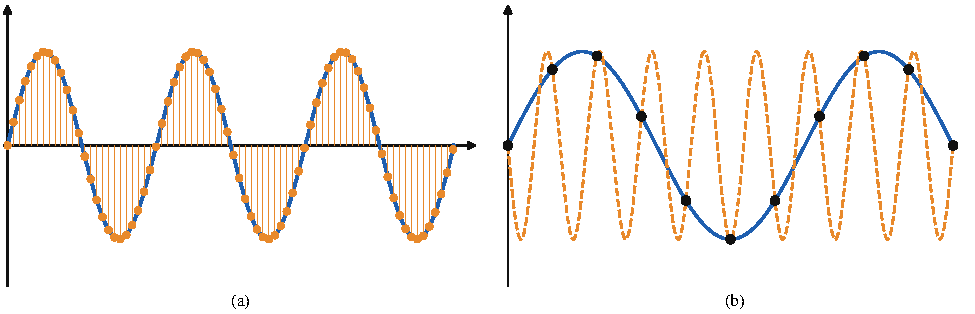
\includegraphics[width=\linewidth]{figures/probkowanie.pdf}
\caption{(a) Sinusoida $440\Hz$ (niebieska) i jej próbki przy $f_s=11\,025\Hz$ (pomarańczowe kropki): około
25 próbek na okres. (b) Aliasing: niebieska sinusoida $0{,}15f_s$ i pomarańczowa przerywana $-\sin$ o częstotliwości
$0{,}85 f_s$ przechodzą przez te same punkty (czarne kropki), więc po spróbkowaniu nie da się ich rozróżnić.}
\label{rys:probkowanie}
\end{figure*}

\begin{naliczbach}
Przy $f_s=11\,025\Hz$ częstotliwość Nyquista wynosi $5512{,}5\Hz$. Najwyższa nuta, którą obsługuje Gen~6,
to MIDI 88 ($1318{,}5\Hz$). Jej trzeci alikwot ($3955{,}5\Hz$) jest jeszcze poniżej Nyquista, ale szósty
($7911\Hz$) już nie. Dlatego HCQT (rozdział~\ref{rozdz:hcqt}) zeruje kanały, w których alikwot wypada powyżej
$0{,}46f_s=5071{,}5\Hz$: tam i tak nie ma wiarygodnej informacji.
\end{naliczbach}

\begin{pulapka}
Nie można „odzyskać” wysokich częstotliwości po zmniejszeniu $f_s$. Przy zmianie próbkowania nagrania
z $44\,100$ na $11\,025\Hz$ trzeba najpierw odfiltrować wszystko powyżej $5512{,}5\Hz$; inaczej aliasing
wmiesza wysokie dźwięki w niskie i sieć zobaczy ,,duchy’’, których w nagraniu nie było.
\end{pulapka}

\section{Półtony, MIDI i centy}

Ucho nie słyszy różnicy częstotliwości, tylko ich \emph{stosunek}: oktawa to zawsze podwojenie. Dlatego
muzycy dzielą oktawę na $12$ równych \emph{stosunkowo} kroków (półtonów).

\haslo{półton}
\begin{definicja}[Skala równomiernie temperowana i numer MIDI]\label{def:midi}
Nutom przypisujemy numery $m\in\mathbb Z$ (\emph{numer MIDI}) tak, że $m=69$ to A4 o częstotliwości $440\Hz$,
a kolejne numery różnią się o jeden półton: stosunek częstotliwości sąsiednich nut jest stały, a po $12$ krokach
częstotliwość się podwaja. Częstotliwość nuty $m$ oznaczamy $f(m)$.
\end{definicja}

\begin{twierdzenie}[Wzór na częstotliwość nuty]\label{tw:fm}
Stosunek częstotliwości sąsiednich półtonów wynosi $2^{1/12}\approx1{,}0595$ oraz
\begin{equation}
  f(m)=440\cdot2^{(m-69)/12}.
  \label{eq:fm}
\end{equation}
\end{twierdzenie}
\begin{pomyslDowodu}
Stały stosunek $r$ i podwojenie po 12 krokach dają $r^{12}=2$; reszta to kolejne mnożenie przez $r$.
\end{pomyslDowodu}
\begin{proof}
Niech $r=f(m+1)/f(m)$ będzie stałe dla każdego $m$. Z definicji \ref{def:midi} po dwunastu krokach częstotliwość się podwaja:
\begin{align*}
f(m+12) &= r^{12}f(m) && \pow{(12 mnożeń przez $r$)}\\
        &= 2f(m)      && \pow{(oktawa)}
\end{align*}
Stąd $r^{12}=2$, czyli $r=2^{1/12}$ (jedyne dodatnie rozwiązanie). Kolejne mnożenie przez $r$ od $m=69$ daje
$f(m)=f(69)\,r^{m-69}=440\cdot2^{(m-69)/12}$, także dla $m<69$ (dzielenie przez $r$). To kończy dowód.
\end{proof}

\begin{table}[ht]
\centering\small
\begin{tabular}{@{}lcccccc@{}}
\toprule
struna & 6 & 5 & 4 & 3 & 2 & 1\\
nuta & E2 & A2 & D3 & G3 & B3 & E4\\
numer MIDI $m$ & 40 & 45 & 50 & 55 & 59 & 64\\
$f(m)$ [Hz] & 82,41 & 110,00 & 146,83 & 196,00 & 246,94 & 329,63\\
\bottomrule
\end{tabular}
\caption{Struny gitary w stroju standardowym i ich częstotliwości z wzoru~\eqref{eq:fm}.}
\label{tab:struny}
\end{table}

\begin{przyklad}[Częstotliwość najniższej struny]\label{prz:e2}
Struna E2 ma $m=40$, więc $f(40)=440\cdot2^{(40-69)/12}=440\cdot2^{-29/12}\approx82{,}41\Hz$. Sprawdzenie:
E2 leży dwie oktawy ($64-40=24=2\cdot12$ półtonów) pod E4, więc $f=329{,}63/2^2=82{,}41\Hz$.
\end{przyklad}

Odstępy mniejsze niż półton mierzymy w \emph{centach}: półton ma $100$ centów.

\haslo{cent}
\begin{definicja}[Cent]\label{def:cent}
Odstęp dwóch dźwięków o częstotliwościach $f_1$ i $f_2$ wynosi
\begin{equation}
  c=1200\,\log_2\frac{f_2}{f_1}\quad\text{centów.}
\end{equation}
\end{definicja}

\begin{przyklad}\label{prz:cent}
Czysta kwinta ($f_2/f_1=3/2$) to $1200\log_2 1{,}5=701{,}96$ centa, czyli prawie dokładnie $7$ półtonów ($700$).
Struna rozstrojona z $440$ do $445\Hz$ jest podwyższona o $1200\log_2(445/440)\approx19{,}6$ centa.
\end{przyklad}

\begin{wniosek}[Centy się dodają]\label{wn:centy-dodaja}
Jeśli $c_{12}$ to odstęp od $f_1$ do $f_2$, a $c_{23}$ od $f_2$ do $f_3$, to odstęp od $f_1$ do $f_3$ wynosi $c_{12}+c_{23}$.
Odstęp jednego półtonu to $100$ centów.
\end{wniosek}
\begin{proof}
\begin{align*}
c_{12}+c_{23} &= 1200\log_2\frac{f_2}{f_1}+1200\log_2\frac{f_3}{f_2} && \pow{(def.~\ref{def:cent})}\\
              &= 1200\log_2\!\Big(\frac{f_2}{f_1}\cdot\frac{f_3}{f_2}\Big) && \pow{(tw.~\ref{tw:log-iloczynu})}\\
              &= 1200\log_2\frac{f_3}{f_1}. && \pow{(skrócenie $f_2$)}
\end{align*}
Dla półtonu $f_2/f_1=2^{1/12}$, więc $c=1200\cdot\tfrac1{12}\log_2 2=100$. Odstępy dodają się jak długości odcinków na osi $\log_2 f$.
\end{proof}

\begin{figure}[ht]
\centering
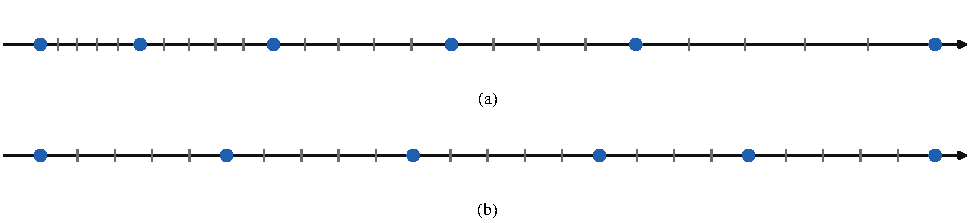
\includegraphics[width=\linewidth]{figures/polsl-osie.pdf}
\sidecaption{Nuty od E2 do E4 (kreski) i sześć strun (niebieskie kropki). (a) Na osi liniowej częstotliwości
odstępy między półtonami rosną: ostatni jest ok.\ 3,8 raza większy niż pierwszy ($2^{23/12}$), więc niskie nuty
tłoczą się przy zerze. (b) Na osi $\log_2 f$ wszystkie półtony są równo oddalone o $1/12$ (z tw.~\ref{tw:log-iloczynu}).
Dlatego model liczy bliskość nut w półtonach, a nie w hercach. \label{rys:polsl-osie}}
\end{figure}

W modelu Gen~6 jedna nuta ma $3$ biny na półton, czyli bin to $100/3\approx33{,}3$ centa. Ewaluacja uznaje
wysokość za poprawną, jeśli różni się od wzorca o mniej niż $50$ centów (ćwierć tonu) --- to ok. półtora biną.

\section{Klatki czasu}

Model nie analizuje całego nagrania naraz, tylko \emph{klatkami}: co $h$ próbek (krok, ang.\ \emph{hop}) bierze okno
długości $N_w$ próbek i liczy z niego widmo (rozdział~\ref{rozdz:fourier}).

\begin{przyklad}[Liczba klatek]\label{prz:klatki}
Gen~6 używa okna $N_w=4096$ próbek ($371{,}5\ms$) i kroku $h=256$ próbek ($23{,}2\ms$). Okno mieści się w nagraniu
o $N$ próbkach dla $t=0,\dots,\lfloor(N-N_w)/h\rfloor$, więc
$T=\lfloor(N-N_w)/h\rfloor+1$. Dla $N=66\,150$ ($6$~s): $T=\lfloor 62\,054/256\rfloor+1=242+1=243$ klatki.
\end{przyklad}

\begin{sprawdz}
\begin{enumerate}
\item Oblicz częstotliwość nuty $m=52$ (E3) i nuty $m=76$. Ile półtonów i ile centów dzieli E3 od E2?
\item Nuta ma częstotliwość $f_1=200\Hz$, a druga $f_2=206\Hz$. Ile centów je dzieli? Czy mieści się w tolerancji $50$ centów?
\item Sinusoida $7000\Hz$ jest próbkowana przy $f_s=11\,025\Hz$. Jaką częstotliwość zobaczy komputer? Skorzystaj z tw.~\ref{tw:aliasing}.
\item Nagranie ma $N=11\,025\cdot 30$ próbek. Ile klatek $T$ daje okno 4096 z krokiem 256?
\end{enumerate}
\end{sprawdz}

\subsection*{Rozwiązania}
\begin{enumerate}
\item $f(52)=440\cdot2^{-17/12}=164{,}81\Hz$ oraz $f(76)=440\cdot 2^{7/12}=659{,}26\Hz$. E3 jest $12$ półtonów, czyli $1200$ centów, nad E2 (stosunek $164{,}81/82{,}41=2$).
\item $c=1200\log_2(206/200)=1200\cdot0{,}0426=51{,}2$ centa, czyli o włos powyżej tolerancji $50$.
\item $f_s-7000=4025\Hz$ (z drugiej części twierdzenia; znak jest przeciwny). Komputer zobaczy ton $4025\Hz$ w przeciwnej fazie.
\item $N=330\,750$ i $(330\,750-4096)/256=1275{,}99\ldots$, więc $T=1275+1=1276$ klatek.
\end{enumerate}

\chapter{Struna gitary i alikwoty}\label{rozdz:alikwoty}

\section{Dlaczego nuta to nie jedna sinusoida?}

Gdy zagramy na gitarze nutę A2, w nagraniu nie ma jednej sinusoidy $110\Hz$. Jest cały szereg sinusoid:
$110$, $220$, $330$, $440$\dots\ Hz. Te dodatkowe składowe nazywamy \emph{alikwotami} (harmonicznymi).
To one nadają instrumentowi barwę, ale też sprawiają największy kłopot w transkrypcji: alikwoty jednej nuty
lądują dokładnie tam, gdzie leżą \emph{inne} nuty. Ten rozdział wyjaśnia, skąd się biorą i dlaczego
na osi logarytmicznej wyglądają jak niezmienny wzorzec --- na tym wzorcu opiera się pierwszy blok sieci Gen~6.

Po tym rozdziale umiesz: (i)~uzasadnić, że struna drga z częstotliwościami $kf_0$, (ii)~wskazać, które nuty
dzielą alikwoty, (iii)~policzyć położenie $h$-tego alikwotu w półtonach i binach, (iv)~wyjaśnić, skąd bierze się
błąd oktawowy.

\section{Drgania własne struny}

Struna o długości $L$ jest zamocowana na obu końcach. Jej wychylenie $u(x,t)$ w punkcie $x\in[0,L]$ i chwili $t$
spełnia równanie falowe $u_{tt}=v^2u_{xx}$, gdzie $v$ to prędkość fali na strunie (zależy od naciągu i masy),
oraz warunki brzegowe $u(0,t)=u(L,t)=0$.

\haslo{fala stojąca}
\begin{definicja}[Fala stojąca (tryb własny)]\label{def:fala-stojaca}
\emph{Falą stojącą} nazywamy rozwiązanie równania falowego postaci $u(x,t)=\phi(x)\cos(2\pi ft)$, w którym
kształt $\phi(x)$ nie zmienia się w czasie, tylko jego wychylenie pulsuje z częstotliwością $f$.
\end{definicja}

\begin{twierdzenie}[Częstotliwości własne struny]\label{tw:struna}
Funkcje
\[u_k(x,t)=\sin\!\Big(\frac{k\pi x}{L}\Big)\cos(2\pi f_k t),\qquad k=1,2,3,\dots,\]
są falami stojącymi spełniającymi równanie falowe i warunki brzegowe wtedy i tylko wtedy, gdy
\begin{equation}
  f_k = k\,\frac{v}{2L}=k f_1 .
\end{equation}
\end{twierdzenie}
\begin{pomyslDowodu}
Wstawiamy $u_k$ do równania $u_{tt}=v^2u_{xx}$, policzymy obie drugie pochodne i porównamy współczynniki.
\end{pomyslDowodu}
\begin{proof}
Warunki brzegowe są spełnione, bo $\sin(0)=0$ oraz $\sin(k\pi)=0$ dla całkowitego $k$. Liczymy pochodne (wzory
$(\sin ax)''=-a^2\sin ax$ i $(\cos bt)''=-b^2\cos bt$ są znane ze szkoły):
\begin{align*}
u_{tt} &= -(2\pi f_k)^2\,u_k, && \pow{(po czasie)}\\
u_{xx} &= -\big(\tfrac{k\pi}{L}\big)^2u_k. && \pow{(po położeniu)}
\end{align*}
Równanie $u_{tt}=v^2u_{xx}$ jest więc równoważne $(2\pi f_k)^2=v^2(k\pi/L)^2$, czyli $2\pi f_k=vk\pi/L$, skąd
$f_k=kv/(2L)$ (bierzemy dodatni pierwiastek, bo $f_k>0$). Dla dowolnego innego $f$ równość nie zachodzi, więc
$f=f_k$ jest warunkiem koniecznym i wystarczającym. Struna może więc drgać z częstotliwościami będącymi całkowitymi
wielokrotnościami najniższej z nich. To kończy dowód.
\end{proof}

Że \emph{każde} drganie struny jest sumą takich fal, orzekł Daniel Bernoulli (rozwinięcie w szereg Fouriera; dowód
wykracza poza zakres tej książki). Dlatego nuta gitary to suma sinusoid:
\begin{equation}
  x(t)=\sum_{h=1}^{H}A_h\sin\big(2\pi\,h f_0\,t+\varphi_h\big),\qquad f_0=f_1,
  \label{eq:szereg-harm}
\end{equation}
gdzie $f_0$ nazywamy \emph{częstotliwością podstawową}, a składową $h=2,3,\dots$ \emph{alikwotem} (dokładnie:
$h$-tą \emph{harmoniczną}). Amplitudy $A_h$ zwykle maleją z $h$, ale nie znikają.

\begin{przyklad}[Najniższa struna]\label{prz:alik-e2}
Struna E2 ($f_0=82{,}41\Hz$) ma długość drgającą $L\approx0{,}65\,$m. Z tw.~\ref{tw:struna} prędkość fali to
$v=2Lf_0\approx 2\cdot0{,}65\cdot82{,}41=107{,}1$~m/s. Alikwoty $h=1,\dots,6$ mają częstotliwości
$82{,}4;\ 164{,}8;\ 247{,}2;\ 329{,}6;\ 412{,}0;\ 494{,}4\Hz$. Alikwot $h=4$ ($329{,}6\Hz$) to dokładnie
częstotliwość nuty E4 --- najwyższej, otwartej struny.
\end{przyklad}

\begin{intuicja}
Struna może drgać jako całość ($k=1$), w dwóch połowach ($k=2$), w trzech trzecich ($k=3$) itd. Każdy sposób
ma swoją częstotliwość i wszystkie występują naraz. Szarpnięcie w środku wzbudza głównie nieparzyste, przy
końcu struny --- bogatszy zestaw.
\end{intuicja}

\begin{pulapka}
Prawdziwa struna jest sztywna, więc jej alikwoty są \emph{nieco wyższe} niż $hf_0$:
$f_h\approx hf_0\sqrt{1+Bh^2}$, gdzie $B\ge0$ to współczynnik nieharmoniczności. Dla $B=10^{-4}$ szósty alikwot
jest za wysoki o $1200\log_2\sqrt{1+36\cdot10^{-4}}\approx3{,}1$ centa, a dla $B=10^{-3}$ o $30{,}6$ centa, prawie cały
bin. Dlatego blok harmoniczny w rozdziale~\ref{rozdz:architektura} ma dodatkowy filtr po sąsiednich binach.
\end{pulapka}

\section{Wspólne alikwoty: skąd błąd oktawowy}

\begin{twierdzenie}[Alikwoty oktawy]\label{tw:oktawa-alik}
Niech nuta $A$ ma częstotliwość podstawową $f_0$, a nuta $B$ częstotliwość $2f_0$ (oktawa wyżej). Wtedy każdy
alikwot nuty $B$ jest alikwotem nuty $A$: $h\cdot 2f_0=(2h)\,f_0$. Odwrotnie nie: nieparzyste alikwoty $A$ nie
są alikwotami $B$.
\end{twierdzenie}
\begin{pomyslDowodu}
Wystarczy przepisać $h\cdot2f_0$ jako $(2h)f_0$ i zauważyć, że $2h$ jest całkowite i parzyste.
\end{pomyslDowodu}
\begin{proof}
Niech $h\in\{1,2,\dots\}$.
\begin{align*}
h\cdot(2f_0) &= (2h)\cdot f_0 && \pow{(łączność mnożenia)}
\end{align*}
Liczba $2h$ jest całkowita, więc $(2h)f_0$ to $2h$-ty alikwot nuty $A$. Natomiast $3f_0$ ($h=3$ dla $A$) byłoby
alikwotem $B$ tylko dla $h'$ spełniającego $h'\cdot2f_0=3f_0$, czyli $h'=1{,}5\notin\mathbb N$. Zatem parzyste
alikwoty $A$ pokrywają się z alikwotami $B$, a nieparzyste nie. To kończy dowód.
\end{proof}

W zwykłym języku: gdy gra E3, w widmie jest wszystko, co zgłosiłoby E2 --- z wyjątkiem co drugiego prążka. A skoro
wyższe alikwoty bywają słabe, E3 do złudzenia przypomina E2 z wyciszonym podstawowym tonem. To jest
\emph{błąd oktawowy}: najtrudniejsza pomyłka w transkrypcji gitary (w naszych pomiarach ok. $24\%$ fałszywych
alarmów klatkowych leży dokładnie oktawę od prawdziwej nuty).

\begin{figure*}[ht]
\centering
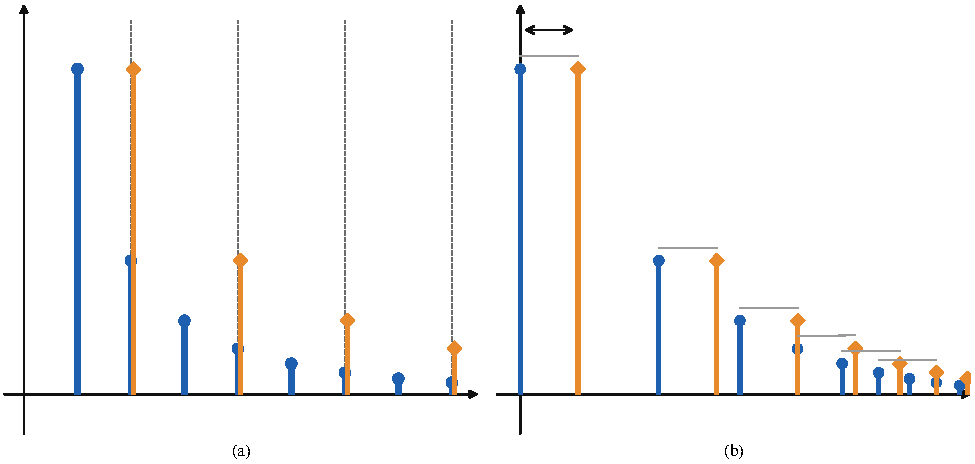
\includegraphics[width=\linewidth]{figures/szereg-alikwotow.pdf}
\caption{Widma szarpniętych strun liczone FFT (wysokość słupka --- amplituda względem prążka podstawowego). (a) Oś liniowa: prążki E2 (niebieskie kółka) i pierwsze cztery prążki E3 (pomarańczowe romby, przesunięte nieco w prawo, żeby były widoczne). Szare przerywane pionowe prowadnice stoją na parzystych prążkach E2: każdy prążek E3 trafia dokładnie w jedną z nich (tw.~\ref{tw:oktawa-alik}).
(b) Oś w półtonach $12\log_2(f/f_{E2})$: wzorzec prążków E2 (niebieskie) i A2 (pomarańczowe) to ta sama figura przesunięta o 5 półtonów (strzałka u góry); cienkie szare łączniki spinają te same numery alikwotów. Kształt zależy tylko od numeru alikwotu, nie od wysokości.}
\label{rys:szereg}
\end{figure*}

\section{Oś logarytmiczna: wzorzec, który się nie zmienia}

Teraz najważniejsze twierdzenie rozdziału. Zmierzmy położenie na osi w półtonach względem ustalonej nuty
odniesienia (np.\ $f_\mathrm{ref}=440\Hz$): $u(f)=12\log_2(f/f_\mathrm{ref})$.

\begin{twierdzenie}[Niezmienniczość wzorca alikwotów]\label{tw:wzorzec}
Jeśli nuta ma częstotliwość podstawową $f_0$ i położenie $u_0=u(f_0)$, to jej $h$-ty alikwot leży w punkcie
\begin{equation}
  u(hf_0)=u_0+12\log_2 h .
\end{equation}
Przesunięcie $12\log_2 h$ zależy od $h$, ale \emph{nie} zależy od $f_0$.
\end{twierdzenie}
\begin{pomyslDowodu}
Logarytm iloczynu jest sumą logarytmów (tw.~\ref{tw:log-iloczynu}): mnożenie przez $h$ staje się dodaniem stałej.
\end{pomyslDowodu}
\begin{proof}
\begin{align*}
u(hf_0) &= 12\log_2\frac{hf_0}{f_\mathrm{ref}} && \pow{(definicja $u$)}\\
        &= 12\log_2 h+12\log_2\frac{f_0}{f_\mathrm{ref}} && \pow{(tw.~\ref{tw:log-iloczynu})}\\
        &= 12\log_2 h+u_0. && \pow{(definicja $u_0$)}
\end{align*}
Stała $12\log_2 h$ nie zawiera $f_0$, więc wzorzec alikwotów ma na tej osi ten sam kształt dla każdej nuty
(rys.~\ref{rys:szereg}b). To kończy dowód.
\end{proof}

\begin{wniosek}[Biny alikwotów]\label{wn:biny}
Przy $3$ binach na półton alikwot $h$ leży o $k_h=36\log_2 h$ binów od podstawy. Zaokrąglone wartości dla
alikwotów używanych w Gen~6:
\begin{center}\small
\begin{tabular}{@{}lccccccc@{}}
\toprule
$h$ & $0{,}5$ & $1$ & $2$ & $3$ & $4$ & $5$ & $6$\\
$12\log_2h$ [półtony] & $-12$ & $0$ & $12$ & $19{,}02$ & $24$ & $27{,}86$ & $31{,}02$\\
$k_h=\round(36\log_2h)$ [biny] & $-36$ & $0$ & $36$ & $57$ & $72$ & $84$ & $93$\\
\bottomrule
\end{tabular}
\end{center}
\end{wniosek}
\begin{proof}
Z tw.~\ref{tw:wzorzec} odstęp w półtonach to $12\log_2h$; przy $3$ binach na półton mnożymy przez $3$:
$k_h=36\log_2h$. Wartości w tabeli to $36\log_2 h$: $36$, $57{,}06$, $72$, $83{,}59$, $93{,}06$ zaokrąglone do
najbliższej liczby całkowitej; np.\ $\round(83{,}59)=84$, a $84$ biny to dokładnie $28$ półtonów, czyli nuta temperowana.
Zaokrąglenie przesuwa więc piąty alikwot o $0{,}41$ bina ($13{,}7$ centa), czyli dokładnie o tyle, o ile ten alikwot
jest za niski względem skali temperowanej.
\end{proof}

\begin{naliczbach}
Struna A2 ($110\Hz$) ma piąty alikwot $550\Hz$. Leży on $12\log_2 5=27{,}86$ półtonów nad A2, czyli blisko nuty
o numerze $45+28=73$ (cis$^{\,3}$, $554{,}4\Hz$), ale o $1200\log_2(550/554{,}4)=-13{,}7$ centa niżej. To nie
błąd modelu, tylko fizyka: trzeci i piąty alikwot nigdy nie trafiają dokładnie w temperowaną skalę.
\end{naliczbach}

\section{Salience: jak wygląda błąd oktawowy w liczbach}

Najprostszy detektor wysokości sumuje energię widma w miejscach, gdzie leżałyby alikwoty kandydata:
$\mathrm{sal}(f)=\frac1H\sum_{h=1}^{H}S(hf)$, gdzie $S$ to amplituda widma. Dla prawdziwej nuty wszystkie składniki są duże.
Ale dla kandydata o oktawę niżej, $f/2$, składniki o parzystym $h$ trafiają w alikwoty prawdziwej nuty, więc salience
też jest wysoka (rys.~\ref{rys:salience}).

\begin{figure}[ht]
\centering
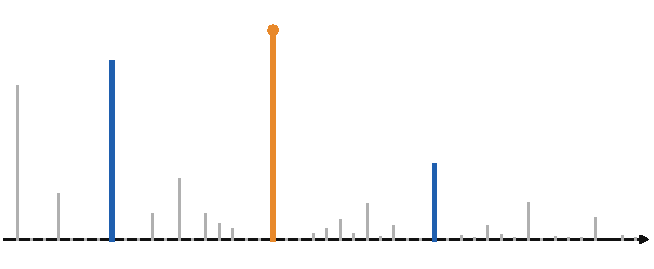
\includegraphics[width=\linewidth]{figures/salience.pdf}
\sidecaption{Salience (suma energii sześciu pierwszych alikwotów, względem największej) dla szarpniętej struny E3 ($m=52$) w funkcji numeru kandydata $m$. Prawdziwa nuta (pomarańczowa) ma najwyższy słupek; pomarańczowa kropkowana pozioma to jej poziom. Kandydat o oktawę niżej ($m=40$, niebieski) jest niewiele niższy, a ten o oktawę wyżej ($m=64$) też się wyróżnia. Szare przerywane pionowe linie to $m=40,52,64$. Wartości liczone z widma FFT jednej nuty. \label{rys:salience}}
\end{figure}

Wniosek praktyczny: samo sumowanie nie wystarcza i trzeba, by sieć porównywała kandydatów \emph{ze sobą}.
Do tego służy uwaga między wysokościami (rozdział~\ref{rozdz:uwaga-wys}).

\section*{Podsumowanie}
\begin{itemize}
\item Struna drga z częstotliwościami $kf_1$ (tw.~\ref{tw:struna}); nuta to suma alikwotów $hf_0$.
\item Prawdziwe struny są lekko nieharmoniczne: $f_h\approx hf_0\sqrt{1+Bh^2}$.
\item Alikwoty nuty o oktawę wyższej zawierają się w alikwotach niższej (tw.~\ref{tw:oktawa-alik}): źródło błędu oktawowego.
\item Na osi półtonów alikwot $h$ leży o $12\log_2h$ nad podstawą, niezależnie od $f_0$ (tw.~\ref{tw:wzorzec}).
\item Przy 3 binach na półton przesunięcia to $-36,0,36,57,72,84,93$ (wn.~\ref{wn:biny}); na nich opiera się blok harmoniczny.
\end{itemize}

\begin{sprawdz}
\begin{enumerate}
\item Wypisz częstotliwości alikwotów $h=1,\dots,8$ struny A2 ($110\Hz$). Które z nich są częstotliwościami podstawowymi nut A3 i E4?
\item Oblicz $12\log_2 7$ i $36\log_2 7$. O ile centów siódmy alikwot odbiega od najbliższej nuty temperowanej?
\item Pokaż, że alikwoty nuty o częstotliwości $3f_0$ (dwunasta wyżej) są alikwotami nuty $f_0$. Które z nich się pokrywają?
\item Struna ma $B=10^{-3}$. O ile centów podwyższony jest alikwot $h=4$? Czy mieści się w jednym binie ($33{,}3$ centa)?
\end{enumerate}
\end{sprawdz}

\subsection*{Rozwiązania}
\begin{enumerate}
\item $110,\,220,\,330,\,440,\,550,\,660,\,770,\,880\Hz$. A3 to $220\Hz$ ($h=2$); E4 to $329{,}6\Hz$, a $330\Hz$ ($h=3$) jest blisko, ale to $E_4$ temperowane ($329{,}63$) tylko w przybliżeniu (o $2$ centy).
\item $12\log_2 7=33{,}69$ półtonów, $36\log_2 7=101{,}06$ binów. Najbliższa nuta jest $34$ półtony wyżej, więc alikwot jest za niski o $0{,}31$ półtonu, czyli $31$ centów.
\item $h\cdot3f_0=(3h)f_0$; pokrywają się alikwoty $h'=3,6,9,\dots$ nuty $f_0$ (co trzeci).
\item $1200\log_2\sqrt{1+16\cdot10^{-3}}=600\log_2(1{,}016)=600\cdot0{,}02289=13{,}7$ centa, więc mieści się w jednym binie ($<33{,}3$).
\end{enumerate}

\chapter{Wektory i macierze}\label{rozdz:wektory}

\section{Dlaczego algebra liniowa?}

Prawie każda warstwa modelu Gen~6 to mnożenie przez macierz. Macierz zamienia jeden wektor cech na inny,
a iloczyn skalarny mierzy, jak bardzo dwa wektory są do siebie podobne; uwaga (rozdział~\ref{rozdz:uwaga})
to nic więcej niż iloczyny skalarne wstawione do softmaksa. Wystarczy nam kilka pojęć, ale musimy je rozumieć
geometrycznie.

Po tym rozdziale umiesz: (i)~policzyć iloczyn skalarny, normę i kąt, (ii)~uzasadnić nierówność Cauchy'ego--Schwarza,
(iii)~pomnożyć macierz przez wektor i dwie macierze przez siebie, (iv)~policzyć liczbę parametrów warstwy liniowej.

\section{Wektor i iloczyn skalarny}

\haslo{iloczyn skalarny}
\begin{definicja}[Iloczyn skalarny i norma]\label{def:iloczyn-skalarny}
Dla wektorów $\vect u,\vect v\in\R^n$ ich \emph{iloczynem skalarnym} jest liczba
\begin{equation}
  \ip{\vect u}{\vect v}=\sum_{i=1}^{n}u_iv_i=\vect u^{\top}\vect v ,
\end{equation}
a \emph{normą} (długością) wektora $\norm{\vect u}=\sqrt{\ip{\vect u}{\vect u}}$.
\end{definicja}

\begin{przyklad}\label{prz:iloczyn}
Dla $\vect u=(2,1,-1)$ i $\vect v=(1,3,2)$: $\ip{\vect u}{\vect v}=2\cdot1+1\cdot3+(-1)\cdot2=3$,
$\norm{\vect u}=\sqrt6\approx2{,}449$, $\norm{\vect v}=\sqrt{14}\approx3{,}742$. Iloczyn skalarny wektora z samym sobą
to kwadrat jego długości: $\ip{\vect u}{\vect u}=4+1+1=6$.
\end{przyklad}

\begin{intuicja}
Iloczyn skalarny pyta: „w ile wektor $\vect u$ jest skierowany tak jak $\vect v$?”. Wynik jest duży i dodatni,
gdy wskazują ten sam kierunek, zero, gdy są prostopadłe, ujemny, gdy przeciwne. W modelu wektor $\vect q$
(„czego szukam”) i wektor $\vect k$ („co mam”) są porównywane właśnie tak.
\end{intuicja}

\begin{twierdzenie}[Cauchy'ego--Schwarza]\label{tw:cs}
Dla dowolnych $\vect u,\vect v\in\R^n$ zachodzi $\abs{\ip{\vect u}{\vect v}}\le\norm{\vect u}\,\norm{\vect v}$, przy czym
równość jest równoważna temu, że wektory są równoległe (jeden jest wielokrotnością drugiego).
\end{twierdzenie}
\begin{pomyslDowodu}
Rozkładamy $\vect v$ na część równoległą do $\vect u$ i prostopadłą do niej. Część prostopadła ma nieujemną długość.
\end{pomyslDowodu}
\begin{proof}
Jeśli $\vect u=\vect0$, obie strony są zerem. Niech $\vect u\neq\vect0$ i niech $\vect p=\dfrac{\ip{\vect u}{\vect v}}{\norm{\vect u}^2}\vect u$
oraz $\vect r=\vect v-\vect p$. Sprawdzamy, że $\vect r\perp\vect u$:
\begin{align*}
\ip{\vect r}{\vect u} &= \ip{\vect v}{\vect u}-\frac{\ip{\vect u}{\vect v}}{\norm{\vect u}^2}\ip{\vect u}{\vect u} && \pow{(liniowość)}\\
 &= \ip{\vect u}{\vect v}-\ip{\vect u}{\vect v}=0. && \pow{($\ip{\vect u}{\vect u}=\norm{\vect u}^2$)}
\end{align*}
Skoro $\vect v=\vect p+\vect r$ z $\vect p\perp\vect r$, to $\norm{\vect v}^2=\norm{\vect p}^2+\norm{\vect r}^2\ge\norm{\vect p}^2$
(Pitagoras). A $\norm{\vect p}^2=\dfrac{\ip{\vect u}{\vect v}^2}{\norm{\vect u}^2}$, więc
\[
\norm{\vect v}^2\ge\frac{\ip{\vect u}{\vect v}^2}{\norm{\vect u}^2}
\quad\Longrightarrow\quad \ip{\vect u}{\vect v}^2\le\norm{\vect u}^2\norm{\vect v}^2 .
\]
Równość zachodzi dokładnie wtedy, gdy $\vect r=\vect0$, czyli $\vect v=\vect p$ jest wielokrotnością $\vect u$.
Pierwiastkowanie obu stron daje tezę.
\end{proof}

W zwykłym języku: iloczyn skalarny nigdy nie jest większy niż iloczyn długości, a największy jest dla wektorów
równoległych. Stąd wynika, że liczba $\cos\theta:=\ip{\vect u}{\vect v}/(\norm{\vect u}\norm{\vect v})$ leży w $[-1,1]$
i można ją nazwać cosinusem kąta $\theta$ między wektorami (rys.~\ref{rys:rzut}). Tę samą nierówność wykorzystamy
w rozdziale~\ref{rozdz:pochodne}, by pokazać, w którą stronę gradient rośnie najszybciej.

\begin{figure}[ht]
\centering
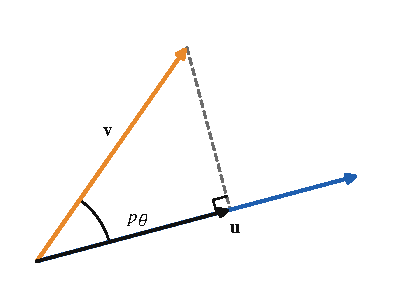
\includegraphics[width=\linewidth]{figures/rzut.pdf}
\sidecaption{Rozkład z dowodu tw.~\ref{tw:cs}. Wektor $\vect v$ (pomarańczowy) rzutujemy na kierunek $\vect u$ (niebieski):
rzut $p$ (czarny) jest równoległy do $\vect u$, a odcinek kreskowany $\vect r=\vect v-\vect p$ jest do niego prostopadły (kąt prosty).
Długość rzutu to $\norm{\vect v}\cos\theta$, więc $\ip{\vect u}{\vect v}=\norm{\vect u}\norm{\vect v}\cos\theta$. \label{rys:rzut}}
\end{figure}

\begin{naliczbach}
Dla wektorów z przykładu~\ref{prz:iloczyn}: $\cos\theta=3/\sqrt{6\cdot14}=3/9{,}165=0{,}327$, czyli $\theta\approx70{,}9^\circ$.
Rzut $\vect v$ na $\vect u$ to $\vect p=\frac{3}{6}\vect u=(1;\,0{,}5;\,-0{,}5)$, a reszta $\vect r=\vect v-\vect p=(0;\,2{,}5;\,2{,}5)$.
Sprawdzenie prostopadłości: $\ip{\vect r}{\vect u}=0\cdot2+2{,}5\cdot1+2{,}5\cdot(-1)=0$. \checkmark
\end{naliczbach}

\begin{pulapka}
Iloczyn skalarny rośnie wraz z długością wektorów, nie tylko z podobieństwem kierunków. Dwa długie, słabo
podobne wektory mogą mieć większy iloczyn niż dwa krótkie, równoległe. Dlatego w uwadze dzielimy iloczyn przez
$\sqrt{d_h}$ (rozdział~\ref{rozdz:uwaga}), a w sieci normalizujemy cechy (rozdział~\ref{rozdz:siec}).
\end{pulapka}

\section{Macierz jako przekształcenie}

\haslo{macierz}
\begin{definicja}[Iloczyn macierzy i wektora]\label{def:macierz-wektor}
Dla macierzy $W\in\R^{m\times n}$ i wektora $\vect x\in\R^n$ wektor $W\vect x\in\R^m$ ma współrzędne
\begin{equation}
  (W\vect x)_i=\sum_{j=1}^{n}W_{ij}x_j=\ip{\vect w_i}{\vect x},
\end{equation}
gdzie $\vect w_i$ to $i$-ty wiersz $W$. Każda współrzędna wyniku to iloczyn skalarny wiersza z wektorem.
\end{definicja}

\begin{przyklad}\label{prz:macierz-wektor}
Niech $W=\begin{pmatrix}1&2\\0&1\\-1&1\end{pmatrix}\in\R^{3\times2}$ i $\vect x=(2,1)$. Wtedy
$W\vect x=(1\cdot2+2\cdot1,\ 0\cdot2+1\cdot1,\ -1\cdot2+1\cdot1)=(4,1,-1)$: wektor z $\R^2$ trafił do $\R^3$.
Dodając wektor obciążenia (ang.\ \emph{bias}) $\vect b=(0{,}5;0;1)$ dostajemy \emph{warstwę liniową}
$W\vect x+\vect b=(4{,}5;\,1;\,0)$.
\end{przyklad}

\begin{intuicja}
Macierz $2\times2$ działa na całą płaszczyznę naraz: prosta zostaje prostą, początek układu zostaje na miejscu, a
siatka kwadratów zamienia się w siatkę równoległoboków. Kolumny $W$ to obrazy wektorów bazowych (rys.~\ref{rys:macierz-siatka}).
\end{intuicja}

\begin{figure*}[ht]
\centering
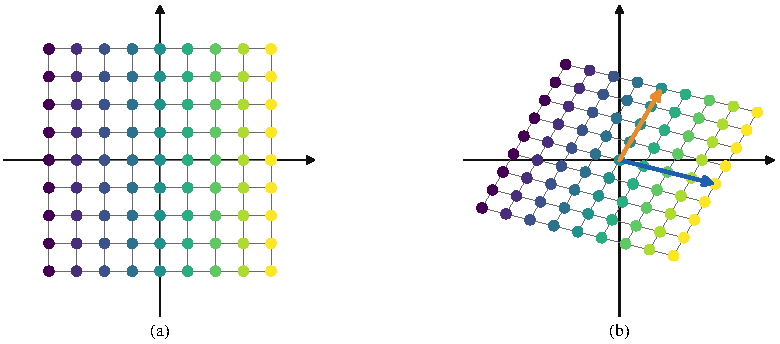
\includegraphics[width=\linewidth]{figures/macierz-siatka.pdf}
\caption{(a) Siatka punktów $9\times9$ w kwadracie $[-1,1]^2$, pokolorowana według współrzędnej $x$ (od fioletu do żółci).
(b) Obraz tej siatki po przekształceniu $\vect x\mapsto A\vect x$ z kolumnami $A\vect e_1$ (niebieska strzałka) i $A\vect e_2$
(pomarańczowa). Kolory pozwalają śledzić każdy punkt: proste zostają prostymi, a pole kwadratu rośnie $\abs{\det A}=1{,}2\cdot1{,}6+0{,}7\cdot0{,}4=2{,}2$ razy.}
\label{rys:macierz-siatka}
\end{figure*}

\begin{twierdzenie}[Mnożenie macierzy to składanie przekształceń]\label{tw:mnozenie}
Dla $A\in\R^{m\times n}$ i $B\in\R^{n\times p}$ macierz $AB\in\R^{m\times p}$ o elementach
$(AB)_{ik}=\sum_{j}A_{ij}B_{jk}$ spełnia $(AB)\vect x=A(B\vect x)$ dla każdego $\vect x\in\R^p$.
\end{twierdzenie}
\begin{pomyslDowodu}
Rozpisujemy obie strony na współrzędne i zamieniamy kolejność sumowania.
\end{pomyslDowodu}
\begin{proof}
\begin{align*}
\big(A(B\vect x)\big)_i &= \sum_{j=1}^{n}A_{ij}\,(B\vect x)_j && \pow{(def.~\ref{def:macierz-wektor})}\\
 &= \sum_{j=1}^{n}A_{ij}\sum_{k=1}^{p}B_{jk}x_k && \pow{(def.~\ref{def:macierz-wektor})}\\
 &= \sum_{k=1}^{p}\Big(\sum_{j=1}^{n}A_{ij}B_{jk}\Big)x_k && \pow{(zmiana kolejności sum)}\\
 &= \sum_{k=1}^{p}(AB)_{ik}\,x_k=\big((AB)\vect x\big)_i. && \pow{(def.\ $AB$)}
\end{align*}
Obie strony mają te same współrzędne, więc są równe. Wymiary zgadzają się, bo $B\vect x\in\R^n$, a $A$ przyjmuje wektory z $\R^n$.
\end{proof}

W zwykłym języku: dwie warstwy liniowe pod rząd to jedna warstwa liniowa o macierzy $AB$. Dlatego sieci wstawiają między
warstwy funkcje nieliniowe (rozdział~\ref{rozdz:siec}); bez nich głębokość nic by nie dała.

\begin{przyklad}[Kolejność ma znaczenie]\label{prz:nieprzemienne}
Dla $A=\begin{pmatrix}1&1\\0&1\end{pmatrix}$ i $B=\begin{pmatrix}2&0\\1&1\end{pmatrix}$ mamy
$AB=\begin{pmatrix}3&1\\1&1\end{pmatrix}$, ale $BA=\begin{pmatrix}2&2\\1&2\end{pmatrix}$. Mnożenie macierzy nie jest przemienne.
\end{przyklad}

\section{Ile parametrów ma warstwa?}

Warstwa liniowa $\vect x\mapsto W\vect x+\vect b$ z $n$ wejściami i $m$ wyjściami ma $mn+m$ parametrów
($W$ ma $mn$ liczb, $\vect b$ ma $m$). To najprostszy rachunek, który będziemy powtarzać w dodatku~\ref{dod:parametry}.

\begin{naliczbach}
Warstwa $64\to256$ (pierwsza w bloku feed-forward modelu Gen~6): $256\cdot64+256=16\,640$ parametrów. Warstwa
$256\to64$: $64\cdot256+64=16\,448$. Razem blok ma $33\,088$ parametrów.
\end{naliczbach}

\section*{Podsumowanie}
\begin{itemize}
\item $\ip{\vect u}{\vect v}=\sum u_iv_i=\norm{\vect u}\norm{\vect v}\cos\theta$ mierzy zgodność kierunków (tw.~\ref{tw:cs}).
\item Rzut $\vect v$ na $\vect u$ to $\frac{\ip{\vect u}{\vect v}}{\norm{\vect u}^2}\vect u$; reszta jest prostopadła do $\vect u$.
\item $W\vect x$: każda współrzędna to iloczyn skalarny wiersza z wektorem; $m\times n$ to $n\to m$.
\item $(AB)\vect x=A(B\vect x)$; mnożenie macierzy nie jest przemienne.
\item Warstwa liniowa $n\to m$ ma $mn+m$ parametrów.
\end{itemize}

\begin{sprawdz}
\begin{enumerate}
\item Dla $\vect u=(1,2,2)$ i $\vect v=(2,0,1)$ policz $\ip{\vect u}{\vect v}$, obie normy i $\cos\theta$. Czy wektory są prostopadłe?
\item Znajdź wektor $\vect w$ prostopadły do $\vect u=(1,2,2)$, taki że $\vect w=(a,1,0)$.
\item Policz $AB$ dla $A=\begin{pmatrix}2&0\\1&1\end{pmatrix}$, $B=\begin{pmatrix}1&3\\0&2\end{pmatrix}$ i sprawdź tw.~\ref{tw:mnozenie} dla $\vect x=(1,1)$.
\item Ile parametrów ma warstwa $159\to48$? A konwolucja $1\times1$ z $336$ kanałów do $48$ (zob.\ rozdz.~\ref{rozdz:siec})?
\end{enumerate}
\end{sprawdz}

\subsection*{Rozwiązania}
\begin{enumerate}
\item $\ip{\vect u}{\vect v}=2+0+2=4$, $\norm{\vect u}=3$, $\norm{\vect v}=\sqrt5$, $\cos\theta=4/(3\sqrt5)=0{,}596$. Nie są prostopadłe (iloczyn $\neq0$).
\item $\ip{\vect u}{\vect w}=a+2=0$, więc $a=-2$ i $\vect w=(-2,1,0)$.
\item $AB=\begin{pmatrix}2&6\\1&5\end{pmatrix}$. $AB\vect x=(8,6)$; $B\vect x=(4,2)$, $A(B\vect x)=(8,\,4+2)=(8,6)$. \checkmark
\item $159\cdot48+48=7680$. Konwolucja $1\times1$ to warstwa liniowa w każdym punkcie: $336\cdot48+48=16\,176$ parametrów.
\end{enumerate}

\chapter{Pochodne, gradient i propagacja wsteczna}\label{rozdz:pochodne}

\section{Jak poprawić model, który się myli?}

Model ma miliony pokręteł, czyli parametrów. Po każdej pomyłce chcemy wiedzieć: \emph{w którą stronę i jak mocno
przekręcić każde pokrętło, żeby błąd zmalał?} Odpowiedzią jest gradient, a narzędziem do jego liczenia reguła łańcuchowa.
Ten rozdział wyprowadza obie rzeczy od początku i pokazuje na malutkiej sieci (jeden neuron), jak wygląda
propagacja wsteczna.

Po tym rozdziale umiesz: (i)~policzyć pochodną złożenia funkcji, (ii)~uzasadnić, że gradient wskazuje kierunek
najszybszego wzrostu, (iii)~zrobić krok spadku gradientu, (iv)~policzyć ręcznie gradient strat dla jednego neuronu
i sprawdzić go numerycznie.

\section{Pochodna funkcji jednej zmiennej}

\haslo{pochodna}
\begin{definicja}[Pochodna]\label{def:pochodna}
\emph{Pochodną} funkcji $f$ w punkcie $x$ nazywamy granicę (o ile istnieje)
\begin{equation}
  f'(x)=\lim_{h\to0}\frac{f(x+h)-f(x)}{h}.
\end{equation}
Liczba $f'(x)$ to nachylenie stycznej do wykresu w punkcie $x$.
\end{definicja}

\begin{przyklad}\label{prz:pochodna-kwadrat}
Dla $f(x)=x^2$: $\dfrac{(x+h)^2-x^2}{h}=\dfrac{2xh+h^2}{h}=2x+h\to 2x$. W punkcie $x=3$ nachylenie wynosi $6$.
Nachylenia siecznych przez $(3,9)$ i $(3+h,(3+h)^2)$ to $7$, $6{,}5$, $6{,}1$, $6{,}01$ dla $h=1;\,0{,}5;\,0{,}1;\,0{,}01$:
zbliżają się do $6$ (rys.~\ref{rys:sieczne}).
\end{przyklad}

\begin{figure}[ht]
\centering
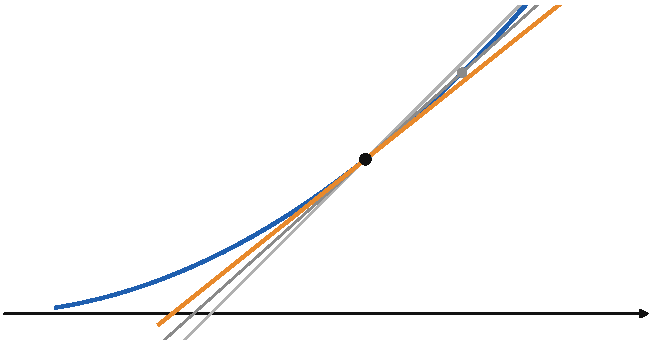
\includegraphics[width=\linewidth]{figures/sieczne.pdf}
\sidecaption{Pochodna jako granica nachyleń. Funkcja $x^2$ (niebieska) i sieczne (szare) przez punkt $(3,9)$ (czarny) i punkty
oddalone o $h=1{,}5$ oraz $0{,}75$. Gdy $h\to0$, sieczna dąży do stycznej (pomarańczowa) o nachyleniu $f'(3)=6$. \label{rys:sieczne}}
\end{figure}

\begin{intuicja}
Pochodna odpowiada na pytanie: „o ile zmieni się wynik, jeśli wejście poruszę o drobinę?”. Zmiana wyniku $\approx f'(x)\cdot$ zmiana wejścia.
To przybliżenie liniowe jest sercem uczenia: nie trzeba znać całej funkcji, wystarczy jej lokalne nachylenie.
\end{intuicja}

Zbierzmy reguły, których użyjemy (pierwsze dwie wynikają wprost z def.~\ref{def:pochodna}):
$(af+bg)'=af'+bg'$, $(fg)'=f'g+fg'$. Najważniejsza jest trzecia.

\begin{twierdzenie}[Reguła łańcuchowa]\label{tw:lancuchowa}
Jeśli $g$ jest różniczkowalna w $x$, a $f$ w $u=g(x)$, to $(f\circ g)'(x)=f'(g(x))\cdot g'(x)$.
\end{twierdzenie}
\begin{pomyslDowodu}
Przybliżamy $g$ prostą o nachyleniu $g'(x)$, a potem $f$ prostą o nachyleniu $f'(u)$. Nachylenia mnożą się.
\end{pomyslDowodu}
\begin{proof}
Różniczkowalność $g$ w $x$ oznacza $g(x+h)-g(x)=g'(x)h+\varepsilon_1(h)h$, gdzie $\varepsilon_1(h)\to0$ przy $h\to0$. Podobnie dla $f$ w $u=g(x)$ i $k=g(x+h)-g(x)$:
$f(u+k)-f(u)=f'(u)k+\varepsilon_2(k)k$, $\varepsilon_2(k)\to0$ przy $k\to0$ (ustalamy $\varepsilon_2(0)=0$). Zatem
\begin{align*}
\frac{f(g(x+h))-f(g(x))}{h} &= \frac{f'(u)\,k+\varepsilon_2(k)\,k}{h} && \pow{(rozwinięcie $f$)}\\
 &= \big(f'(u)+\varepsilon_2(k)\big)\cdot\frac{k}{h} && \pow{(wyłączenie $k$)}\\
 &= \big(f'(u)+\varepsilon_2(k)\big)\big(g'(x)+\varepsilon_1(h)\big). && \pow{($k/h$ z rozwinięcia $g$)}
\end{align*}
Gdy $h\to0$, to $k\to0$ (bo $g$ jest ciągła), więc $\varepsilon_1,\varepsilon_2\to0$ i całość dąży do $f'(u)g'(x)$. To kończy dowód.
\end{proof}

W zwykłym języku: pochodna złożenia to iloczyn pochodnych kolejnych etapów. Sieć neuronowa to długie złożenie, więc jej pochodna to długi iloczyn.

\begin{twierdzenie}[Pochodna sigmoidy]\label{tw:pochodna-sigmoidy}
Funkcja $\sigma(z)=\dfrac{1}{1+e^{-z}}$ spełnia $\sigma'(z)=\sigma(z)\big(1-\sigma(z)\big)$.
\end{twierdzenie}
\begin{pomyslDowodu}
Zapisujemy $\sigma=(1+e^{-z})^{-1}$ i stosujemy regułę łańcuchową.
\end{pomyslDowodu}
\begin{proof}
Niech $u=1+e^{-z}$, więc $\sigma=u^{-1}$, $\dfrac{d\sigma}{du}=-u^{-2}$ i $\dfrac{du}{dz}=-e^{-z}$. Z tw.~\ref{tw:lancuchowa}:
\begin{align*}
\sigma'(z) &= -u^{-2}\cdot(-e^{-z})=\frac{e^{-z}}{(1+e^{-z})^2} && \pow{(reguła łańcuchowa)}\\
 &= \frac{1}{1+e^{-z}}\cdot\frac{e^{-z}}{1+e^{-z}} && \pow{(rozbicie)}\\
 &= \sigma(z)\Big(1-\frac{1}{1+e^{-z}}\Big)=\sigma(z)\big(1-\sigma(z)\big). && \pow{($\tfrac{e^{-z}}{1+e^{-z}}=1-\sigma$)}
\end{align*}
Pochodną można więc policzyć z samej wartości $\sigma$, bez ponownego liczenia wykładnika. To kończy dowód.
\end{proof}

Największa pochodna wynosi $\sigma'(0)=\tfrac12\cdot\tfrac12=\tfrac14$; dla $|z|$ dużego pochodna dąży do zera
(\emph{nasycenie}) --- to jedna z przyczyn, dla których głębokie sieci z samymi sigmoidami uczą się wolno.

\section{Gradient i spadek gradientu}

\haslo{gradient}
\begin{definicja}[Pochodna cząstkowa i gradient]\label{def:gradient}
Dla $f\colon\R^n\to\R$ \emph{pochodna cząstkowa} $\partial f/\partial x_i$ to pochodna po $x_i$ przy pozostałych współrzędnych
traktowanych jak stałe. \emph{Gradient} to wektor tych pochodnych:
$\nabla f(\vect x)=\big(\tfrac{\partial f}{\partial x_1},\dots,\tfrac{\partial f}{\partial x_n}\big)$.
\end{definicja}

\begin{przyklad}\label{prz:gradient}
Dla $f(x,y)=x^2+3xy$: $\partial f/\partial x=2x+3y$, $\partial f/\partial y=3x$. W punkcie $(1,2)$ gradient to $(8,3)$
o długości $\sqrt{73}\approx8{,}54$. Zwiększenie $x$ o $0{,}01$ zwiększa $f$ o ok.\ $0{,}08$, zwiększenie $y$ o $0{,}01$ o ok.\ $0{,}03$.
\end{przyklad}

\begin{twierdzenie}[Gradient wskazuje kierunek najszybszego wzrostu]\label{tw:gradient-najszybszy}
Niech $f$ będzie różniczkowalna w $\vect x$ i $\nabla f(\vect x)\neq\vect0$. Wśród wektorów jednostkowych $\vect d$ pochodna kierunkowa
$\frac{d}{dt}f(\vect x+t\vect d)\big|_{t=0}$ jest największa dla $\vect d=\nabla f/\norm{\nabla f}$ i wynosi wtedy $\norm{\nabla f}$.
\end{twierdzenie}
\begin{pomyslDowodu}
Reguła łańcuchowa zamienia pochodną kierunkową na iloczyn skalarny $\ip{\nabla f}{\vect d}$, a tu działa nierówność Cauchy'ego--Schwarza (tw.~\ref{tw:cs}).
\end{pomyslDowodu}
\begin{proof}
Niech $\phi(t)=f(\vect x+t\vect d)$. Z reguły łańcuchowej dla wielu zmiennych (każda współrzędna zależy od $t$ z pochodną $d_i$):
\begin{align*}
\phi'(0) &= \sum_{i=1}^{n}\frac{\partial f}{\partial x_i}\,d_i && \pow{(reguła łańcuchowa)}\\
 &= \ip{\nabla f(\vect x)}{\vect d}\le\norm{\nabla f}\,\norm{\vect d}=\norm{\nabla f}. && \pow{(tw.~\ref{tw:cs}, $\norm{\vect d}=1$)}
\end{align*}
Równość w Cauchy'ego--Schwarza zachodzi, gdy $\vect d$ jest równoległy do $\nabla f$, czyli $\vect d=\nabla f/\norm{\nabla f}$ (dodatnia wielokrotność, żeby wynik był dodatni).
Wtedy $\phi'(0)=\ip{\nabla f}{\nabla f}/\norm{\nabla f}=\norm{\nabla f}$. To kończy dowód.
\end{proof}

W zwykłym języku: stoisz na zboczu i chcesz iść w górę jak najszybciej --- idź wzdłuż gradientu. Chcemy \emph{zmniejszać}
stratę, więc idziemy \emph{przeciwnie}.

\begin{definicja}[Spadek gradientu]\label{def:spadek}
Dla funkcji straty $L(\vect\theta)$ i \emph{kroku uczenia} $\eta>0$ kolejne przybliżenia to
$\vect\theta_{k+1}=\vect\theta_k-\eta\,\nabla L(\vect\theta_k)$.
\end{definicja}

\begin{naliczbach}
Weźmy $L(x,y)=\tfrac12(x^2+10y^2)$, $\nabla L=(x,10y)$ i start $(1,1)$. Dla $\eta=0{,}05$ kolejne punkty to
$(0{,}95;0{,}5)$, $(0{,}902;0{,}25)$, $(0{,}857;0{,}125)$: schodzimy gładko, ale wolno wzdłuż $x$. Dla $\eta=0{,}15$:
$(0{,}85;-0{,}5)$, $(0{,}722;0{,}25)$, $(0{,}614;-0{,}125)$: współrzędna $y$ zmienia znak w każdym kroku
(zygzak) i jest dwa razy mniejsza w kolejnych krokach. Dla $\eta=0{,}21$ zygzak rośnie i metoda się rozbiega
(dlaczego, wyjaśnia tw.~\ref{tw:eta} w rozdziale~\ref{rozdz:optymalizacja}).
\end{naliczbach}

\begin{figure*}[ht]
\centering
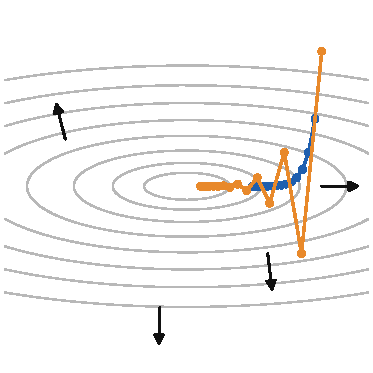
\includegraphics[width=0.88\linewidth]{figures/spadek.pdf}
\caption{Spadek gradientu dla $L=\tfrac12(x^2+10y^2)$ (szare warstwice) z punktu $(1,1)$. Czarne strzałki to gradient w kilku punktach:
zawsze prostopadły do warstwicy i skierowany pod górę, więc krok idzie w przeciwną stronę. Niebieska ścieżka ($\eta=0{,}05$, 14 kroków)
schodzi gładko, ale wolno; pomarańczowa ($\eta=0{,}15$) przeskakuje przez dolinę i zygzakuje. Obie obliczone programem.}
\label{rys:spadek}
\end{figure*}

\section{Propagacja wsteczna na jednym neuronie}

\begin{przyklad}[Gradient strat dla neuronu]\label{prz:backprop}
Neuron: $z=wx+b$, $\hat y=\sigma(z)$, strata $L=(\hat y-y)^2$. Dane: $x=2$, $w=0{,}5$, $b=-0{,}3$, cel $y=1$.
\emph{Przód:} $z=0{,}7$, $\hat y=\sigma(0{,}7)=0{,}6682$, $L=(0{,}6682-1)^2=0{,}1101$.
\emph{Tył} (reguła łańcuchowa, od wyniku ku wejściu):
\begin{align*}
\frac{\partial L}{\partial\hat y} &= 2(\hat y-y)=-0{,}6636,\\
\frac{\partial\hat y}{\partial z} &= \hat y(1-\hat y)=0{,}2217 && \pow{(tw.~\ref{tw:pochodna-sigmoidy})}\\
\frac{\partial L}{\partial w} &= \frac{\partial L}{\partial\hat y}\cdot\frac{\partial\hat y}{\partial z}\cdot\frac{\partial z}{\partial w}
 =(-0{,}6636)(0{,}2217)(2)=-0{,}2943,\\
\frac{\partial L}{\partial b} &= (-0{,}6636)(0{,}2217)(1)=-0{,}1471.
\end{align*}
Sprawdzenie numeryczne: $\big(L(w+10^{-6})-L(w-10^{-6})\big)/(2\cdot10^{-6})=-0{,}2943$. \checkmark
Ujemny gradient oznacza, że \emph{zwiększenie} $w$ zmniejsza stratę: neuron powinien być bardziej pewny odpowiedzi $1$.
\end{przyklad}

\begin{intuicja}
Propagacja wsteczna to reguła łańcuchowa wykonana od końca: zaczynamy od „jak strata zależy od wyniku” i cofając się
przez każdą operację, mnożymy przez jej lokalną pochodną. Każda warstwa musi znać tylko własną pochodną i gradient
przychodzący z góry; dzięki temu da się to zautomatyzować dla dowolnej sieci (PyTorch robi dokładnie to).
\end{intuicja}

\begin{pulapka}
Gradient policzony ręcznie warto \emph{zawsze} porównać z ilorazem różnicowym (jak wyżej). Błąd znaku albo brakującego czynnika
nie powoduje awarii, tylko powolne, dziwne uczenie, które trudno zdiagnozować. Granice stosowalności: różnica $10^{-6}$ w
\texttt{float64} jest dobra; w \texttt{float32} zbyt mały krok tonie w błędach zaokrągleń.
\end{pulapka}

\section*{Podsumowanie}
\begin{itemize}
\item Pochodna to nachylenie stycznej; zmiana wyniku $\approx f'(x)\cdot$ zmiana wejścia.
\item Reguła łańcuchowa: pochodna złożenia to iloczyn pochodnych (tw.~\ref{tw:lancuchowa}); $\sigma'=\sigma(1-\sigma)$.
\item Gradient to wektor pochodnych cząstkowych i wskazuje kierunek najszybszego wzrostu (tw.~\ref{tw:gradient-najszybszy}).
\item Spadek gradientu: $\vect\theta\leftarrow\vect\theta-\eta\nabla L$; za duży krok powoduje zygzak i rozbieżność.
\item Propagacja wsteczna to reguła łańcuchowa liczona od wyniku w stronę wejść; wynik sprawdzamy ilorazem różnicowym.
\end{itemize}

\begin{sprawdz}
\begin{enumerate}
\item Policz pochodną $f(x)=\sigma(3x-1)$ w $x=0$. (Wskazówka: tw.~\ref{tw:lancuchowa} i \ref{tw:pochodna-sigmoidy}.)
\item Dla $f(x,y)=x^2+3xy$ w punkcie $(1,2)$ podaj kierunek jednostkowy najszybszego wzrostu i wartość pochodnej kierunkowej w tym kierunku.
\item Wykonaj jeden krok spadku gradientu z $(1,2)$ dla $L=x^2+3xy$ i $\eta=0{,}01$. O ile (w przybliżeniu) zmieni się $L$?
\item Neuron z przykładu~\ref{prz:backprop} ma $y=0$ zamiast $1$. Jaki jest teraz $\partial L/\partial w$?
\end{enumerate}
\end{sprawdz}

\subsection*{Rozwiązania}
\begin{enumerate}
\item $\sigma(-1)=0{,}2689$, więc $f'(0)=3\sigma(-1)(1-\sigma(-1))=3\cdot0{,}2689\cdot0{,}7311=0{,}590$.
\item $\nabla f=(8,3)$, kierunek $(8,3)/8{,}544=(0{,}936;\,0{,}351)$, pochodna kierunkowa $\norm{\nabla f}=8{,}544$.
\item Krok: $(1,2)-0{,}01(8,3)=(0{,}92;\,1{,}97)$. $L(1,2)=1+6=7$; $L(0{,}92;1{,}97)=0{,}8464+5{,}4372=6{,}2836$. Zmiana $\approx-0{,}716$ (przybliżenie liniowe: $-\eta\norm{\nabla f}^2=-0{,}01\cdot73=-0{,}73$).
\item $\partial L/\partial\hat y=2(0{,}6682-0)=1{,}3364$, więc $\partial L/\partial w=1{,}3364\cdot0{,}2217\cdot2=0{,}5926$ (dodatni: $w$ należy \emph{zmniejszyć}).
\end{enumerate}

\chapter{Transformata Fouriera: z drgań do widma}\label{rozdz:fourier}

\section{Co jest w tym nagraniu?}

Nagranie to ciąg liczb zmieniających się w czasie. Nas interesuje coś innego: \emph{jakie częstotliwości w nim
grają?} Odpowiada na to transformata Fouriera, która rozkłada sygnał na sinusoidy. Dla krótkiego okna dźwięku
zamienia $N$ próbek w $N$ liczb mówiących, ile energii niesie każda częstotliwość. To jest pierwszy krok liczenia cech
Gen~6 (rozdział~\ref{rozdz:hcqt}). Poznamy jej własności i, co ważne, \emph{ograniczenia}: przeciek i skończoną rozdzielczość.

Po tym rozdziale umiesz: (i)~policzyć DFT małego sygnału ręcznie, (ii)~uzasadnić, że wiąże ona sinusoidy z pojedynczymi prążkami,
(iii)~wyjaśnić, czemu stosuje się okno Hanna, (iv)~policzyć rozdzielczość $f_s/N$ i ocenić, czy dwa dźwięki da się rozdzielić.

\section{Liczby zespolone w dwóch zdaniach}

\haslo{wzór Eulera}
\begin{definicja}[Jednostka urojona i wzór Eulera]\label{def:euler}
Liczba $i$ spełnia $i^2=-1$. Dla rzeczywistego $\theta$ definiujemy
$e^{i\theta}=\cos\theta+i\sin\theta$ --- punkt na okręgu jednostkowym o kącie $\theta$.
Moduł $\abs{a+ib}=\sqrt{a^2+b^2}$. Zachodzi $e^{i\alpha}e^{i\beta}=e^{i(\alpha+\beta)}$ oraz $\abs{e^{i\theta}}=1$.
\end{definicja}

\begin{przyklad}\label{prz:euler}
$e^{i\pi}=\cos\pi+i\sin\pi=-1$, $e^{i\pi/2}=i$, $e^{-i\pi/2}=-i$. Zatem
$\cos\theta=\tfrac12(e^{i\theta}+e^{-i\theta})$ i $\sin\theta=\tfrac1{2i}(e^{i\theta}-e^{-i\theta})$ --- sinus i cosinus to
„składowe” punktu na okręgu.
\end{przyklad}

\section{Dyskretna transformata Fouriera}

\haslo{DFT}
\begin{definicja}[DFT]\label{def:dft}
Dla ciągu $x[0],\dots,x[N-1]$ jego \emph{dyskretna transformata Fouriera} to ciąg liczb zespolonych
\begin{equation}
  X[k]=\sum_{n=0}^{N-1}x[n]\,e^{-2\pi i\,kn/N},\qquad k=0,1,\dots,N-1.
  \label{eq:dft}
\end{equation}
Numer $k$ odpowiada częstotliwości $f_k=k\,f_s/N$; $\abs{X[k]}$ nazywamy \emph{widmem amplitudowym}.
Odstęp $\Delta f=f_s/N$ między sąsiednimi $k$ to \emph{rozdzielczość} (szerokość binu) DFT.
\end{definicja}

\begin{przyklad}[$N=4$ ręcznie]\label{prz:dft4}
Niech $x=(1,0,-1,0)$, czyli jeden okres cosinusa w $4$ próbkach. Ponieważ $e^{-2\pi ikn/4}=(-i)^{kn}$:
$X[0]=1+0-1+0=0$; $X[1]=1+(-1)(-i)^{2}=1+1=2$; $X[2]=1+(-1)(-i)^{4}=1-1=0$; $X[3]=1+(-1)(-i)^{6}=1+1=2$.
Widmo $\abs{X}=(0,2,0,2)$: cosinus daje dwa prążki, w $k=1$ i lustrzany $k=3=N-1$. Przy $f_s=4\Hz$ prążek $k=1$ to $1\Hz$.
\end{przyklad}

\begin{intuicja}
$X[k]$ mierzy, jak bardzo sygnał „zgadza się” z sinusoidą o $k$ obiegach na okno: mnożymy sygnał przez tę sinusoidę i
sumujemy (to iloczyn skalarny z rozdziału~\ref{rozdz:wektory}!). Gdy sygnał ją zawiera, wszystkie składniki sumy dodają się;
gdy nie, wzajemnie się znoszą.
\end{intuicja}

\begin{twierdzenie}[Ortogonalność sinusoid]\label{tw:ortogonalnosc}
Dla całkowitych $k,l$:
\begin{equation}
  \sum_{n=0}^{N-1}e^{2\pi i(k-l)n/N}=\begin{cases}N,&k\equiv l\pmod N,\\0,&\text{w przeciwnym razie.}\end{cases}
\end{equation}
\end{twierdzenie}
\begin{pomyslDowodu}
To suma wyrazów ciągu geometrycznego o ilorazie $q=e^{2\pi i(k-l)/N}$, a $q^N=1$.
\end{pomyslDowodu}
\begin{proof}
Niech $q=e^{2\pi i(k-l)/N}$. Gdy $k\equiv l\pmod N$, to $q=1$ i suma ma $N$ składników równych $1$, czyli wynosi $N$.
W przeciwnym razie $q\neq1$ i ze wzoru na sumę ciągu geometrycznego
\begin{align*}
\sum_{n=0}^{N-1}q^n &= \frac{1-q^N}{1-q} && \pow{(suma geometryczna)}\\
 &= \frac{1-e^{2\pi i(k-l)}}{1-q}=\frac{1-1}{1-q}=0. && \pow{($q^N=e^{2\pi i(k-l)}=1$)}
\end{align*}
Sinusoidy o różnych numerach są więc wzajemnie prostopadłe (iloczyn skalarny zero), a o tym samym mają „długość” $\sqrt N$. To kończy dowód.
\end{proof}

\begin{wniosek}[DFT sinusoidy o całkowitej liczbie okresów]\label{wn:dft-cos}
Jeśli $x[n]=A\cos(2\pi k_0n/N)$ dla całkowitego $0<k_0<N/2$, to $X[k_0]=X[N-k_0]=AN/2$, a pozostałe $X[k]=0$.
\end{wniosek}
\begin{proof}
Z przykładu~\ref{prz:euler}: $x[n]=\tfrac A2\big(e^{2\pi ik_0n/N}+e^{-2\pi ik_0n/N}\big)$. Wstawiamy do \eqref{eq:dft}:
\begin{align*}
X[k] &= \frac A2\sum_{n}e^{2\pi i(k_0-k)n/N}+\frac A2\sum_{n}e^{-2\pi i(k_0+k)n/N} && \pow{(rozdzielność)}\\
     &= \frac A2\,N\,\indic{k=k_0}+\frac A2\,N\,\indic{k=N-k_0}. && \pow{(tw.~\ref{tw:ortogonalnosc})}
\end{align*}
Dla $N=4$, $k_0=1$, $A=1$ daje to $X[1]=X[3]=2$, zgodnie z przykładem~\ref{prz:dft4}. Czysty ton daje więc dokładnie jeden prążek (i jego lustro).
\end{proof}

\section{Przeciek i okno}

Jest haczyk: wniosek~\ref{wn:dft-cos} wymaga, by ton miał \emph{całkowitą} liczbę okresów w oknie. Częstotliwości
nut tego nie spełniają. Co się dzieje, gdy $k_0$ nie jest całkowite?

\begin{twierdzenie}[Przeciek]\label{tw:przeciek}
Niech $x[n]=e^{2\pi i\,\kappa n/N}$ z dowolnym rzeczywistym $\kappa$ i niech $\delta=\kappa-k$. Wtedy
\begin{equation}
  \abs{X[k]}=\left|\frac{\sin(\pi\delta)}{\sin(\pi\delta/N)}\right|.
\end{equation}
Jest to $N$ dla $\delta=0$, zero dla niezerowych całkowitych $\delta$ i ok.\ $\frac{2}{\pi}N\approx0{,}64N$ dla $\delta=\tfrac12$
(dla dużych $N$).
\end{twierdzenie}
\begin{pomyslDowodu}
To znów suma geometryczna, tym razem z ilorazem $e^{2\pi i\delta/N}\neq1$; moduł licznika i mianownika daje sinusy.
\end{pomyslDowodu}
\begin{proof}
Z \eqref{eq:dft} i definicji $\delta$:
\begin{align*}
X[k] &= \sum_{n=0}^{N-1}e^{2\pi i\delta n/N}=\frac{1-e^{2\pi i\delta}}{1-e^{2\pi i\delta/N}} && \pow{(suma geometryczna)}\\
 &= \frac{e^{i\pi\delta}\,(e^{-i\pi\delta}-e^{i\pi\delta})}{e^{i\pi\delta/N}\,(e^{-i\pi\delta/N}-e^{i\pi\delta/N})} && \pow{(wyłączenie połówek kątów)}\\
 &= e^{i\pi\delta(1-1/N)}\,\frac{\sin(\pi\delta)}{\sin(\pi\delta/N)}. && \pow{(wzór Eulera na sinus)}
\end{align*}
Moduł czynnika $e^{i\cdots}$ wynosi $1$, więc zostaje podany wzór. Dla $\delta=0$ granica to $N$; dla całkowitego $\delta\neq0$ licznik jest zerem; dla $\delta=\frac12$ mianownik $\sin(\pi/2N)\approx\pi/2N$, a licznik $1$, czyli $\approx2N/\pi$. To kończy dowód.
\end{proof}

W zwykłym języku: ton między binami „rozlewa się” na sąsiednie prążki i traci w najgorszym miejscu ok.\ $3{,}9\dB$ głośności ($20\log_{10}(2/\pi)=-3{,}9\dB$). Poza tym ogony przecieku opadają wolno: pierwszy listek boczny okna prostokątnego to tylko $-13\dB$.
Silny ton zasłoni więc słabe składowe daleko od siebie. Rozwiązaniem jest okno.

\haslo{okno Hanna}
\begin{definicja}[Okno Hanna]\label{def:hann}
\emph{Oknem Hanna} nazywamy $w[n]=\tfrac12\big(1-\cos(2\pi n/N)\big)$, $n=0,\dots,N-1$. Przed liczeniem DFT mnożymy próbki przez $w[n]$.
\end{definicja}

\begin{przyklad}\label{prz:hann}
Dla $N=8$: $w=(0;\,0{,}146;\,0{,}5;\,0{,}854;\,1;\,0{,}854;\,0{,}5;\,0{,}146)$: okno łagodnie zaczyna się od zera, osiąga $1$ w środku i znów opada.
Brzegi okna nie są więc ucinane gwałtownie, a to właśnie nagła krawędź powoduje długi ogon przecieku.
\end{przyklad}

\begin{twierdzenie}[Widmo okna Hanna]\label{tw:hann}
Jeśli $Y[k]$ jest DFT sygnału $y[n]$ z oknem prostokątnym, to DFT sygnału $y[n]w[n]$ z oknem Hanna wynosi
$\tfrac12Y[k]-\tfrac14Y[k-1]-\tfrac14Y[k+1]$.
\end{twierdzenie}
\begin{pomyslDowodu}
Zapisujemy $w[n]=\tfrac12-\tfrac14e^{2\pi in/N}-\tfrac14e^{-2\pi in/N}$ i zauważamy, że mnożenie przez $e^{2\pi in/N}$ przesuwa widmo o jeden bin.
\end{pomyslDowodu}
\begin{proof}
Z wzoru Eulera $\cos(2\pi n/N)=\tfrac12\big(e^{2\pi in/N}+e^{-2\pi in/N}\big)$, więc
$w[n]=\tfrac12-\tfrac14e^{2\pi in/N}-\tfrac14e^{-2\pi in/N}$. Dla składnika z $e^{2\pi in/N}$:
\begin{align*}
\sum_n y[n]e^{2\pi in/N}e^{-2\pi ikn/N} &= \sum_n y[n]e^{-2\pi i(k-1)n/N}=Y[k-1]. && \pow{(złączenie wykładników)}
\end{align*}
Analogicznie $e^{-2\pi in/N}$ daje $Y[k+1]$. Z liniowości DFT otrzymujemy podany wzór. To kończy dowód.
\end{proof}

Skutki (to już obserwacja liczbowa, rys.~\ref{rys:przeciek}, a nie część dowodu): kopie z $k\pm1$ mają znak przeciwny niż środkowa, więc
kasują ogon przecieku, a główny listek robi się szerszy ($4$ biny między zerami zamiast $2$). Pierwszy listek boczny
spada z $-13{,}3\dB$ (okno prostokątne) do $-31{,}5\dB$.

\begin{figure*}[ht]
\centering
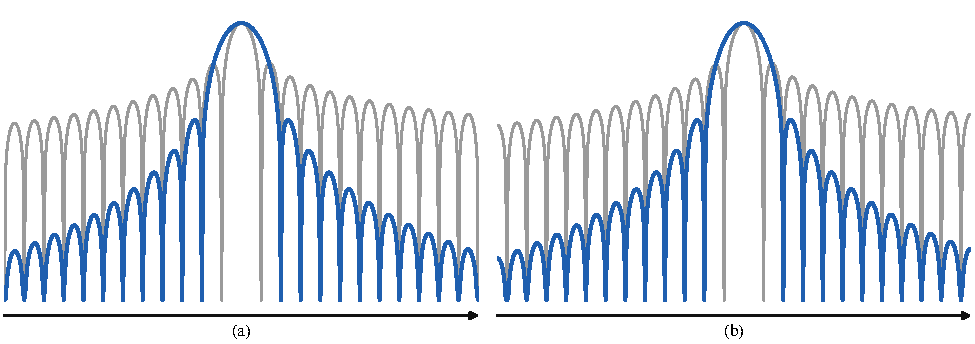
\includegraphics[width=\linewidth]{figures/przeciek.pdf}
\caption{Widmo tonu z $N=128$ próbek w decybelach (skala od $-80$ do $0\dB$, wspólna). Ton dokładnie w prążku (linia ciągła) i w połowie między prążkami (przerywana). (a) Okno prostokątne (szare): wąski pik, ale listki boczne opadają wolno; pierwszy ma $-13\dB$ (pomarańczowa kropkowana). (b) Okno Hanna (niebieskie): pik dwa razy szerszy, ale pierwszy listek tylko $-31\dB$ (pomarańczowa kropkowana), a dalsze opadają szybko. Ton między prążkami ma niższy pik w obu oknach.}
\label{rys:przeciek}
\end{figure*}

\begin{pulapka}
Okno Hanna nie jest za darmo: rozszerza główny listek dwukrotnie, więc \emph{pogarsza rozdzielczość}. Zyskujemy czystość widma
(brak „duchów” od silnych tonów), tracimy zdolność do rozdzielania dwóch bliskich dźwięków. Wybór okna to zawsze kompromis.
\end{pulapka}

\section{Rozdzielczość: kiedy dwa dźwięki są jednym}

Gen~6 liczy FFT dla okna $N=4096$ przy $f_s=11\,025\Hz$ (czas $372\ms$), więc $\Delta f=2{,}69\Hz$; główny listek Hanna ma
$\pm2\Delta f=\pm5{,}4\Hz$. Zero-padding (dopisanie zer, rozdział~\ref{rozdz:hcqt}) dzieli siatkę na $0{,}67\Hz$, ale
\emph{nie zwiększa rozdzielczości} --- tylko interpoluje ten sam kształt.

\begin{naliczbach}
Najniższe nuty gitary leżą blisko siebie: E2 ($82{,}41\Hz$) i F2 ($87{,}31\Hz$) dzieli $4{,}9\Hz$, mniej niż $5{,}4\Hz$ połowy głównego listka.
Numerycznie (rys.~\ref{rys:rozdzielczosc}a) widmo sumy z oknem $4096$ ma dwa „piki” w $84{,}1$ i $85{,}5\Hz$: to artefakt interferencji,
nie prawdziwe położenia nut. Dla E2 i F\#2 ($10{,}1\Hz$ różnicy) piki są już rozdzielone i leżą w $82{,}8$ i $92{,}2\Hz$, czyli mniej niż $0{,}4\Hz$ od prawdy (b).
Okno $N=1024$ ($\Delta f=10{,}8\Hz$) daje dla pary (b) dwa piki w błędnych miejscach ($78{,}1$ i $96{,}9\Hz$).
\end{naliczbach}

\begin{figure*}[ht]
\centering
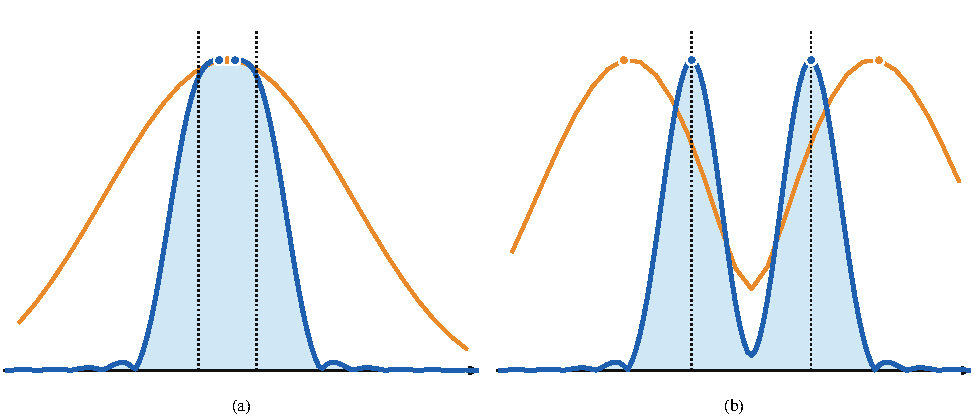
\includegraphics[width=\linewidth]{figures/rozdzielczosc.pdf}
\caption{Widmo (okno Hanna) sumy dwóch sinusoid; czarne kropkowane pionowe linie to prawdziwe częstotliwości, kropki to znalezione piki. Niebieskie z wypełnieniem: okno $N=4096$; pomarańczowe: $N=1024$. (a) E2 i F2 (półton, $4{,}9\Hz$): długie okno daje dwa bliskie piki w złych miejscach (interferencja), krótkie jeden szeroki pagórek. (b) E2 i F\#2 ($10{,}1\Hz$): długie okno rozdziela tony prawie bez błędu położenia, krótkie daje dwa piki odsunięte od prawdy o kilka herców. Dlatego model dostaje dwa okna --- długie dla wysokości, krótkie dla czasu --- i uczy się łączyć wskazówki z wielu klatek.}
\label{rys:rozdzielczosc}
\end{figure*}

Wniosek jest uczciwy i ważny: z samego widma jednej klatki nie da się wiarygodnie odróżnić sąsiednich niskich półtonów.
Dlatego dalsze rozdziały dodają kontekst w czasie (uwaga między klatkami) i szereg alikwotów (wyższe alikwoty są szerzej rozstawione
w hercach, więc łatwiej je rozdzielić).

\section*{Podsumowanie}
\begin{itemize}
\item DFT $X[k]=\sum x[n]e^{-2\pi ikn/N}$; bin $k$ to $kf_s/N$ Hz; rozdzielczość $\Delta f=f_s/N$.
\item Sinusoidy o różnych $k$ są ortogonalne (tw.~\ref{tw:ortogonalnosc}); ton o całkowitej liczbie okresów daje jeden prążek.
\item Ton między binami „przecieka” (tw.~\ref{tw:przeciek}); okno prostokątne ma listki $-13\dB$.
\item Okno Hanna to trzy przesunięte kopie okna prostokątnego (tw.~\ref{tw:hann}): listki $-31\dB$, ale główny listek dwa razy szerszy.
\item Dla $N=4096$ rozdzielczość to $2{,}7\Hz$, a sąsiednie niskie półtony (odstęp $4{,}9\Hz$) nie rozdzielają się czysto.
\end{itemize}

\begin{sprawdz}
\begin{enumerate}
\item Policz ręcznie DFT dla $x=(1,1,0,0)$ ($N=4$) i podaj widmo amplitudowe.
\item Ile wynosi $\Delta f$ dla $N=1024$ i $N=16\,384$ przy $f_s=11\,025\Hz$? Który z nich ma większą \emph{rozdzielczość} i dlaczego $N=16\,384$ z zero-paddingiem z $4096$ nie jest dokładniejszy niż $4096$?
\item Ton $A\cos(2\pi\cdot 10\,n/64)$ ma $N=64$. Które $k$ mają niezerowe $X[k]$ i ile wynosi $\abs{X}$ dla $A=2$?
\item Pokaż, że $\sum_{n=0}^{N-1}w[n]=N/2$ dla okna Hanna (wskazówka: tw.~\ref{tw:ortogonalnosc} z $k=l\pm1$).
\end{enumerate}
\end{sprawdz}

\subsection*{Rozwiązania}
\begin{enumerate}
\item $X[k]=1+e^{-2\pi ik/4}=1+(-i)^k$: $X[0]=2$, $X[1]=1-i$, $X[2]=0$, $X[3]=1+i$. $\abs{X}=(2,\sqrt2,0,\sqrt2)$.
\item $\Delta f=10{,}77\Hz$ i $0{,}673\Hz$. Zero-padding z $4096$ do $16\,384$ daje siatkę $0{,}673\Hz$, ale okno nadal trwa $372\ms$, więc rozdzielczość pozostaje $2{,}69\Hz$ (główny listek tak samo szeroki). Prawdziwe $N=16\,384$ próbek (1,5 s) miałoby $\Delta f=0{,}673\Hz$ \emph{prawdziwej} rozdzielczości.
\item $k=10$ i $k=54$; $\abs{X}=AN/2=2\cdot64/2=64$.
\item $\sum w=\tfrac12N-\tfrac14\sum e^{2\pi in/N}-\tfrac14\sum e^{-2\pi in/N}=\tfrac N2-0-0=\tfrac N2$, bo sumy z $k-l=\pm1$ są zerami.
\end{enumerate}

\chapter{HCQT: widmo ułożone harmonicznie}\label{rozdz:hcqt}

\section{Pomysł: niech każdy kandydat widzi swoje alikwoty w jednym miejscu}

Mamy widmo $\abs{X[k]}$ okna dźwięku (rozdział~\ref{rozdz:fourier}) i wiemy, że nuta to szereg alikwotów (rozdział~\ref{rozdz:alikwoty}).
Chcemy, żeby sieć uczyła się ,,wzorca nuty''. Gdyby ułożyć widmo tak, by dla \emph{każdego kandydata na wysokość} wszystkie jego
alikwoty leżały w tym samym miejscu tensora, zwykła konwolucja (rozdział~\ref{rozdz:siec}) mogłaby je porównywać bez żadnej
kombinatoryki. Tak działa HCQT (ang.\ \emph{harmonic constant-Q transform}): to stos kopii widma, z których $h$-ta jest „ściśnięta” $h$-krotnie.
Nasz opis opiera się na pomyśle Bittnera i in.\ (2017).

Po tym rozdziale umiesz: (i)~zdefiniować wartość HCQT w binie $p$ kanału $h$, (ii)~policzyć decybele i normalizację,
(iii)~udowodnić, że cechy nie zależą od głośności nagrania, (iv)~udowodnić, że kanały to przesunięte kopie jednego widma, (v)~odczytać kształt $X\in\R^{T\times9\times159}$.

\section{Biny logarytmiczne i alikwoty}

Zamiast równych odstępów w hercach (jak w DFT) używamy równych odstępów w \emph{półtonach}: wprost z rozdziału~\ref{rozdz:alikwoty} wiemy, że wtedy
wzorzec alikwotów jest niezmienniczy względem przesunięcia.

\haslo{bin logarytmiczny}
\begin{definicja}[Bin wysokości i jego częstotliwość]\label{def:bin}
Niech $b=3$ (liczba binów na półton) i $m_{\min}=36$. Bin o numerze $p=0,1,\dots,158$ ma wysokość
$m_p=m_{\min}+\dfrac{p-1}{3}$ (w skali MIDI) i częstotliwość środkową $f(p)=440\cdot2^{(m_p-69)/12}$. Bin $p=3s+1$ jest środkiem półtonu $s=0,\dots,52$ (nuta MIDI $36+s$);
biny $3s$ i $3s+2$ leżą $33{,}3$ centa niżej i wyżej.
\end{definicja}

\begin{przyklad}\label{prz:bin}
Nuta E2 ($m=40$, $s=4$) leży w binie $p=3\cdot4+1=13$: $m_{13}=36+12/3=40$ i $f=82{,}41\Hz$. Biny $12$ i $14$ to $m=39{,}67$ i $40{,}33$, czyli $\mp33$ centy od E2.
Zakres wszystkich $159$ binów to $m=35{,}67$ do $88{,}33$.
\end{przyklad}

\haslo{HCQT}
\begin{definicja}[Wartość HCQT]\label{def:hcqt}
Niech $S_t[k]$ będzie widmem amplitudowym okna o środku w klatce $t$ (okno Hanna, FFT z zero-paddingiem $\times4$).
Dla \emph{numeru alikwotu} $h\in\{0{,}5;1;2;3;4;5\}$ definiujemy amplitudę w binie $p$:
\begin{equation}
  A_h[t,p]=\max\Big\{S_t[k]\;:\;h f(p)\,2^{-1/72}\le f_k\le h f(p)\,2^{1/72}\Big\}.
\end{equation}
Przedział to $\pm\frac1{6}$ półtonu (czyli $\frac{1}{72}$ oktawy) wokół częstotliwości $hf(p)$. Zakres jest pusty ($A_h:=0$), gdy $hf(p)>0{,}46f_s$ (ponad Nyquistem).
\end{definicja}

\begin{przyklad}\label{prz:hcqt-przedzial}
Dla $p=13$ (E2, $f=82{,}41\Hz$) i $h=2$ szukamy maksimum widma w przedziale $[2\cdot82{,}41\cdot2^{-1/72},\,2\cdot82{,}41\cdot2^{1/72}]=[163{,}3;\ 166{,}4]\Hz$ wokół drugiego alikwotu ($164{,}8\Hz$).
Przy zero-paddingu $\times4$ bin FFT ma $0{,}67\Hz$, więc przedział zawiera ok.\ $5$ binów FFT, a $A_2[t,13]$ to największa z ich amplitud.
\end{przyklad}

\begin{intuicja}
$A_h[t,p]$ odpowiada na pytanie: „gdyby w binie $p$ grała nuta, a ja podsłuchałbym jej $h$-ty alikwot --- ile energii bym tam usłyszał?”.
Kanał $h=1$ to zwykłe widmo, kanał $h=2$ pokazuje, ile energii jest o oktawę wyżej niż każdy kandydat, itd.
\end{intuicja}

\section{Decybele i normalizacja}

Ucho ocenia głośność logarytmicznie (rozdział~\ref{rozdz:zapis}), więc amplitudy zamieniamy na decybele.

\haslo{decybel}
\begin{definicja}[Decybel i cecha]\label{def:db}
Poziom amplitudy $A>0$ w decybelach to $L=20\log_{10}A\;\dB$. Dla ustalonej \emph{referencji} $L_\mathrm{ref}$ definiujemy \emph{cechę}
\begin{equation}
  \varphi=\clip\!\Big(\frac{L-L_\mathrm{ref}}{60}+1,\;0,\;1{,}3\Big).
\end{equation}
Referencją jest $99{,}5$. percentyl wszystkich poziomów $L$ nagrania (osobno dla okna długiego i krótkiego).
\end{definicja}

\begin{naliczbach}
Niech $L_\mathrm{ref}=-20\dB$ (czyli $A_\mathrm{ref}=0{,}1$). Piksel o $A=0{,}1$ ma $\varphi=1$. Piksel o $A=10^{-3}$ ($L=-60\dB$):
$\varphi=(-60+20)/60+1=0{,}333$. Piksel o $A=0{,}12$ ($L=-18{,}4\dB$): $\varphi=1{,}026$ (cecha bywa $>1$, bo $A$ może przewyższać
percentyl). Piksel o $A=10^{-5}$ ($L=-100\dB$): $\varphi=-0{,}333$, po przycięciu $0$. Zakres $60\dB$ znaczy: wszystko cichsze niż $60\dB$ poniżej referencji to dla sieci cisza.
\end{naliczbach}

\begin{twierdzenie}[Niezależność od głośności nagrania]\label{tw:glosnosc}
Niech nagranie $x$ zostanie pomnożone przez stałą $g>0$. Pomijając wpływ stałej $10^{-9}$ w logarytmie, cechy $\varphi$ obliczone dla $gx$ i dla $x$ są identyczne.
\end{twierdzenie}
\begin{pomyslDowodu}
Skalowanie sygnału dodaje stałą do wszystkich decybeli, a percentyl przesuwa się o tę samą stałą; różnica $L-L_\mathrm{ref}$ się nie zmienia.
\end{pomyslDowodu}
\begin{proof}
Widmo jest liniowe w sygnale, więc $S_t[k]\mapsto gS_t[k]$, a maksimum z dodatnich liczb też się skaluje: $A\mapsto gA$ (maksimum jest jednorodne). Zatem
\begin{align*}
L' &= 20\log_{10}(gA)=L+20\log_{10}g && \pow{(tw.~\ref{tw:log-iloczynu})}\\
L'_\mathrm{ref} &= \mathrm{perc}_{99{,}5}\{L+c\}=L_\mathrm{ref}+c, \quad c=20\log_{10}g && \pow{(percentyl przesuwa się o $c$)}\\
L'-L'_\mathrm{ref} &= L-L_\mathrm{ref}. && \pow{($c$ się skraca)}
\end{align*}
Cecha zależy tylko od $L-L_\mathrm{ref}$, więc jest taka sama. Percentyl przesuwa się o $c$, bo dodanie stałej nie zmienia kolejności elementów.
\end{proof}

W zwykłym języku: czy nagranie jest ciche, czy głośne, sieć dostaje te same liczby. Jeżeli $g=3$, wszystkie poziomy rosną o $20\log_{10}3=9{,}54\dB$, a referencja o tyle samo. Numerycznie
(rys.~\ref{rys:niezmiennik}b) dla nagrania i nagrania $10$ razy cichszego największa różnica cech to $4\cdot10^{-5}$, czyli błąd zaokrągleń \texttt{float32}.

\begin{figure*}[ht]
\centering
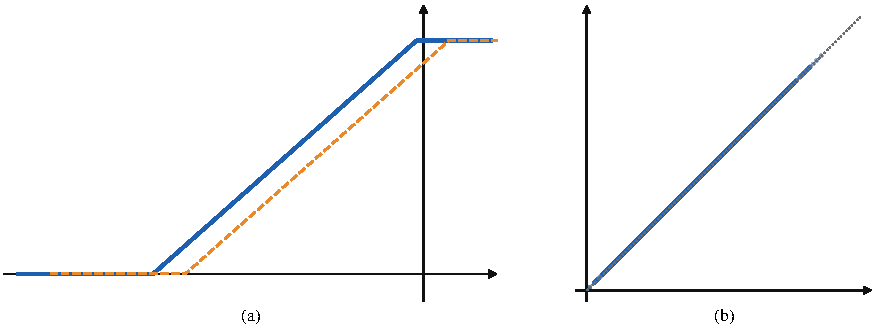
\includegraphics[width=0.9\linewidth]{figures/niezmiennik-glosnosci.pdf}
\caption{(a) Cecha jako funkcja $\log_{10}A$ (niebieska): płaski początek (cisza poniżej $60\dB$ od referencji), liniowy wzrost i przycięcie na $1{,}3$.
Nagranie 3 razy głośniejsze (pomarańczowa przerywana) ma tę samą krzywą, bo referencja przesuwa się razem z poziomami (tw.~\ref{tw:glosnosc}).
(b) Wartości cech tego samego nagrania (poziomo) i nagrania 10 razy cichszego (pion): wszystkie punkty leżą na przekątnej (kropkowana).}
\label{rys:niezmiennik}
\end{figure*}

\begin{pulapka}
Niezależność od głośności dotyczy \emph{stałego} przeskalowania całego nagrania. Nie obejmuje szumu: jeśli głośniejsza jest tylko jedna część,
albo tło ma stały poziom, normalizacja nie pomoże. Stała $10^{-9}$ w logarytmie psuje twierdzenie tylko dla amplitud tak małych, że i tak są obcięte do zera.
\end{pulapka}

\section{Kanały to przesunięte kopie jednego widma}

\begin{twierdzenie}[Przesunięcie kanałów]\label{tw:przesuniecie-kanalow}
Jeśli $k_h=36\log_2h$ jest liczbą całkowitą, to dla każdej klatki i każdego binu $p$ zachodzi $A_h[t,p]=A_1[t,p+k_h]$.
\end{twierdzenie}
\begin{pomyslDowodu}
Bin $p+k_h$ ma częstotliwość środkową dokładnie $h$ razy większą niż bin $p$, więc obie amplitudy to maksimum z tego samego przedziału widma.
\end{pomyslDowodu}
\begin{proof}
Z def.~\ref{def:bin} mamy $m_{p+k_h}=m_p+k_h/3$. Zatem
\begin{align*}
f(p+k_h) &= 440\cdot2^{(m_p+k_h/3-69)/12}=f(p)\cdot2^{k_h/36} && \pow{(dodanie wykładników)}\\
 &= f(p)\cdot2^{\log_2h}=h\,f(p). && \pow{($k_h=36\log_2h$)}
\end{align*}
Przedział w def.~\ref{def:hcqt} dla $A_h[t,p]$ to $[hf(p)2^{-1/72},\,hf(p)2^{1/72}]$, a dla $A_1[t,p+k_h]$ to $[f(p+k_h)2^{-1/72},\,f(p+k_h)2^{1/72}]$; są identyczne.
Maksimum z tego samego zbioru jest to samo. (Rozważamy tylko $p$, dla których $p+k_h$ mieści się w $0,\dots,158$.) To kończy dowód.
\end{proof}

Dla $h=0{,}5;2;4$ mamy $k_h=-36;36;72$, więc równość jest dokładna; dla $h=3$ i $5$ ($k_h=57{,}06$ i $83{,}59$) przesunięcie całkowite
jest tylko przybliżeniem, a błąd to poniżej pół bina. Sprawdziliśmy to na prawdziwym kodzie: dla kanałów $h=0{,}5;2;4$ różnica
$A_h[t,p]-A_1[t,p+k_h]$ wynosi dokładnie $0$ w całym nagraniu, a dla $h=3$ średnio $0{,}007$ (maksymalnie $0{,}18$). Ta własność uzasadnia
blok harmoniczny sieci (rozdział~\ref{rozdz:architektura}): sieć sama może „doprzesunąć” własne cechy o $k_h$ binów i uzyskać alikwoty także wyższe niż $5$.

\section{Co dokładnie dostaje sieć}

\begin{table}[ht]
\centering\small
\begin{tabular}{@{}lll@{}}
\toprule
parametr & wartość & znaczenie\\
\midrule
$f_s$ & $11\,025\Hz$ & po zmianie próbkowania\\
okna & $4096$ i $1024$ próbek & długie (wysokość), krótkie (czas)\\
krok & $256$ próbek $=23{,}2\ms$ & odstęp klatek\\
zero-padding & $\times4$ & gładsze położenie pików\\
alikwoty długie & $0{,}5;1;2;3;4;5$ & kanały $1$--$6$\\
alikwoty krótkie & $1;2;3$ & kanały $7$--$9$\\
biny & $3\times53=159$ & MIDI $36$--$88$\\
normalizacja & $99{,}5$ perc., $60\dB$, clip $1{,}3$ & def.~\ref{def:db}\\
\bottomrule
\end{tabular}
\caption{Parametry HCQT w modelu Gen~6. Wynik: $X\in\R^{T\times9\times159}$.}
\label{tab:hcqt-param}
\end{table}

\begin{figure*}[ht]
\centering
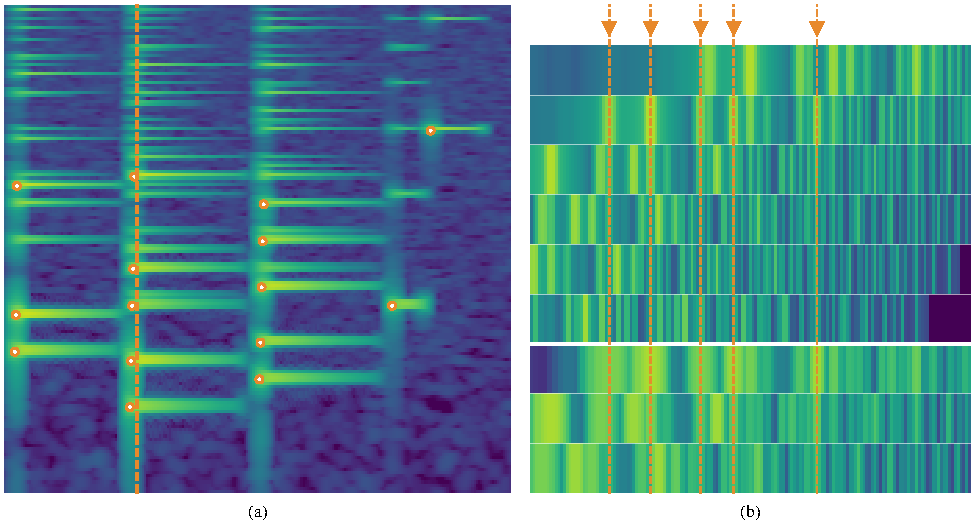
\includegraphics[width=\linewidth]{figures/hcqt-przyklad.pdf}
\caption{HCQT syntetycznego, 6-sekundowego nagrania gitary. (a) Kanał $h=1$: czas poziomo ($243$ klatki), wysokość pionowo ($159$ binów); jasne ślady to alikwoty grających nut, kółka z pomarańczowym brzegiem to początki prawdziwych nut, pomarańczowa przerywana linia to klatka pokazana w (b). (b) Cała jedna klatka: $9$ kanałów (wiersze; gruba biała linia oddziela $6$ kanałów okna długiego od $3$ okna krótkiego) $\times$ $159$ binów (kolumny). Pomarańczowe trójkąty i przerywane pionowe linie wskazują kolumny prawdziwych nut: w każdej z nich jasne plamy pojawiają się w wielu kanałach naraz, bo alikwoty kandydata ustawiono w jednej kolumnie.}
\label{rys:hcqt-przyklad}
\end{figure*}

W obu oknach analizujemy tę samą klatkę $t$ (środek wspólny). Dla nagrania 6-sekundowego $T=243$ i $X$ ma $243\cdot9\cdot159=347\,733$ liczby (przykład~\ref{prz:tensor-hcqt}).
Rysunek~\ref{rys:hcqt-przyklad}b to najważniejszy obrazek książki: siatka nut jako kolumny, siedem „pięter” alikwotów jako wiersze. Zadaniem sieci jest rozpoznać w tej siatce
wzorzec „ta kolumna jest zajęta przez nutę” i odróżnić go od kolumn, które tylko udają nutę, bo leżą oktawę niżej.

\section*{Podsumowanie}
\begin{itemize}
\item Bin wysokości ma $\tfrac13$ półtonu; $p=3s+1$ jest środkiem półtonu $s$.
\item $A_h[t,p]$ to maksimum widma wokół $hf(p)$ ($\pm\frac16$ półtonu); $h=0{,}5\dots5$ (okno długie), $1,2,3$ (krótkie): razem $9$ kanałów.
\item Cecha $=\clip((L-L_\mathrm{ref})/60+1,0,1{,}3)$ jest niezależna od głośności nagrania (tw.~\ref{tw:glosnosc}).
\item Jeśli $36\log_2h$ jest całkowite, kanał $h$ to kanał $1$ przesunięty o tyle binów (tw.~\ref{tw:przesuniecie-kanalow}).
\item Wejście sieci to $X\in\R^{T\times9\times159}$ ze krokiem $23{,}2\ms$.
\end{itemize}

\begin{sprawdz}
\begin{enumerate}
\item O ile decybeli rośnie poziom, gdy amplituda podwaja się? A gdy rośnie $10$ razy?
\item Dla $L_\mathrm{ref}=-30\dB$ policz cechę piksela o $A=0{,}005$. (Wskazówka: $L=20\log_{10}A$.)
\item Który bin odpowiada nucie A2 ($m=45$)? Jaki jest numer binu jej trzeciego alikwotu $(h=3)$, w przybliżeniu całkowitym?
\item Od jakiej wysokości kanał $h=5$ jest zerowy? Użyj progu $0{,}46f_s$ i podaj najniższy bin $p$, dla którego tak jest.
\end{enumerate}
\end{sprawdz}

\subsection*{Rozwiązania}
\begin{enumerate}
\item $20\log_{10}2=6{,}02\dB$, a $20\log_{10}10=20\dB$.
\item $L=20\log_{10}0{,}005=-46{,}02\dB$, $\varphi=(-46{,}02+30)/60+1=0{,}733$.
\item $p=3\cdot(45-36)+1=28$. Trzeci alikwot: $k_3=\round(36\log_2 3)=57$, czyli bin $28+57=85$ ($m_{85}=36+84/3=64$, to E4; dokładnie oczekiwane $45+19{,}02=64{,}02$).
\item Zero, gdy $5f(p)>5071{,}5\Hz$, czyli $f(p)>1014{,}3\Hz$, czyli $m_p>69+12\log_2(1014{,}3/440)=83{,}48$. Z $m_p=36+(p-1)/3$ dostajemy $p-1>142{,}4$, więc najniższy zerowy bin to $p=144$. Zerowych jest więc $159-144=15$ binów (najwyższe $5$ półtonów: ok.\ $83{,}5$--$88{,}3$).
\end{enumerate}

\chapter{Prawdopodobieństwo i funkcje straty}\label{rozdz:strata}

\section{Jak powiedzieć modelowi, że się myli?}

Wyjściem sieci jest, dla każdej klatki i półtonu, liczba z przedziału $(0,1)$: „z jakim prawdopodobieństwem w tej klatce gra ta nuta?”.
Żeby uczyć sieć gradientem (rozdział~\ref{rozdz:pochodne}), potrzebujemy funkcji straty: jednej liczby, która jest mała, gdy odpowiedzi
są dobre, i duża, gdy złe. Tu wyprowadzimy dwie funkcje używane w Gen~6 (sigmoidę z entropią krzyżową dla początków, ramek i końców; softmax dla tabulatury)
i pokażemy, \emph{dlaczego} akurat takie.

Po tym rozdziale umiesz: (i)~zamienić liczbę rzeczywistą na prawdopodobieństwo sigmoidą i softmaksem, (ii)~policzyć stratę BCE i jej gradient,
(iii)~uzasadnić, że BCE jest najmniejsza dla prawdziwego prawdopodobieństwa, (iv)~powiedzieć, co robi waga klasy dodatniej.

\section{Sigmoida i softmax}

\haslo{sigmoida}
\begin{definicja}[Sigmoida]\label{def:sigmoida}
Funkcja $\sigma(z)=\dfrac1{1+e^{-z}}$ przekształca dowolną liczbę $z\in\R$ (zwaną \emph{logitem}) w liczbę z przedziału $(0,1)$.
Zachodzi $\sigma(-z)=1-\sigma(z)$ i $\sigma(0)=\tfrac12$.
\end{definicja}

\begin{przyklad}\label{prz:sigmoida}
$\sigma(0)=0{,}5$; $\sigma(2)=0{,}881$; $\sigma(-2)=0{,}119$; $\sigma(-3)=0{,}0474$. Duży dodatni logit oznacza „prawie na pewno tak”, duży ujemny
„prawie na pewno nie”. Odwrotność: $z=\ln\frac{p}{1-p}$ (logarytm szans).
\end{przyklad}

\haslo{softmax}
\begin{definicja}[Softmax]\label{def:softmax}
Dla wektora logitów $\vect z\in\R^K$ (K klas) \emph{softmaksem} nazywamy wektor o współrzędnych
$\softmax(\vect z)_i=\dfrac{e^{z_i}}{\sum_{j=1}^{K}e^{z_j}}$.
\end{definicja}

\begin{przyklad}\label{prz:softmax}
Dla $\vect z=(2;1;0{,}1)$ mamy $e^{z}=(7{,}389;\,2{,}718;\,1{,}105)$, suma $11{,}212$, więc softmax to $(0{,}659;\,0{,}242;\,0{,}099)$.
Największy logit dostaje największe prawdopodobieństwo, ale mniejsze też nie giną.
\end{przyklad}

\begin{twierdzenie}[Własności softmaksa]\label{tw:softmax}
Dla każdego $\vect z$: (a) $\softmax(\vect z)_i>0$ i $\sum_i\softmax(\vect z)_i=1$; (b) $\softmax(\vect z+c\vect 1)=\softmax(\vect z)$ dla dowolnej stałej $c$.
\end{twierdzenie}
\begin{pomyslDowodu}
(a) wynika z dodatniości wykładnika i z tego, że dzielimy przez sumę; (b): czynnik $e^c$ skraca się w liczniku i mianowniku.
\end{pomyslDowodu}
\begin{proof}
(a) $e^{z_i}>0$ dla każdego $z_i$, a mianownik jest sumą takich liczb, więc wynik jest dodatni; suma ułamków o wspólnym mianowniku $\sum_j e^{z_j}$ daje $1$.
(b)
\begin{align*}
\frac{e^{z_i+c}}{\sum_j e^{z_j+c}} &= \frac{e^{c}e^{z_i}}{e^{c}\sum_j e^{z_j}} && \pow{($e^{a+b}=e^ae^b$)}\\
 &= \frac{e^{z_i}}{\sum_j e^{z_j}}. && \pow{(skrócenie $e^c$)}
\end{align*}
W praktyce odejmujemy od logitów ich maksimum ($c=-\max z$), żeby uniknąć przepełnienia $e^{z}$ dla dużych $z$ --- wynik się nie zmienia. To kończy dowód.
\end{proof}

Sigmoida to softmax dwóch klas $(z,0)$: $\softmax(z,0)_1=e^z/(e^z+1)=\sigma(z)$. Używamy sigmoidy, gdy klasy nie wykluczają się (w jednej klatce może grać wiele półtonów naraz), a softmaksu, gdy
dokładnie jedna odpowiedź jest prawdziwa (na strunie dokładnie jedna z $21$ klas: milczy albo któryś próg).

\section{Entropia krzyżowa}

\haslo{entropia krzyżowa}
\begin{definicja}[Strata BCE]\label{def:bce}
Dla prawdopodobieństwa $p\in(0,1)$ i etykiety $y\in[0,1]$ (zwykle $0$ lub $1$) \emph{binarna entropia krzyżowa} wynosi
\begin{equation}
  \ell(p,y)=-\big[\,y\ln p+(1-y)\ln(1-p)\,\big].
\end{equation}
Z \emph{wagą klasy dodatniej} $\alpha>0$: $\ell_\alpha(p,y)=-\big[\alpha\,y\ln p+(1-y)\ln(1-p)\big]$.
\end{definicja}

\begin{przyklad}\label{prz:bce}
Dla $y=1$ i $p=0{,}9$: $\ell=-\ln0{,}9=0{,}105$. Dla $p=0{,}2$: $\ell=-\ln0{,}2=1{,}609$; z wagą $\alpha=4$ strata wynosi $6{,}44$. Dla $y=0$ i $p=0{,}2$: $\ell=-\ln0{,}8=0{,}223$.
Pewność w złą stronę ($p\to0$ przy $y=1$) jest karana nieograniczenie: $-\ln p\to\infty$ (rys.~\ref{rys:bce}a).
\end{przyklad}

\begin{intuicja}
Strata BCE to „zaskoczenie” modelu: $-\ln p$ to ile bitów (nat) informacji niesie zdarzenie, któremu przypisaliśmy $p$. Model, który
był pewien złej odpowiedzi, jest bardzo zaskoczony, więc ponosi dużą karę.
\end{intuicja}

\begin{twierdzenie}[Gradient BCE po logicie]\label{tw:grad-bce}
Dla $p=\sigma(z)$: $\dfrac{\partial\ell}{\partial z}=\sigma(z)-y$. Z wagą $\alpha$: $\dfrac{\partial\ell_\alpha}{\partial z}=(\alpha y+1-y)\,\sigma(z)-\alpha y$.
\end{twierdzenie}
\begin{pomyslDowodu}
Regułą łańcuchową przez $p=\sigma(z)$ i pochodną sigmoidy $\sigma'=\sigma(1-\sigma)$ (tw.~\ref{tw:pochodna-sigmoidy}); czynniki $p(1-p)$ się skracają.
\end{pomyslDowodu}
\begin{proof}
Niech $p=\sigma(z)$, więc $\partial p/\partial z=p(1-p)$. Dla $\ell_\alpha$:
\begin{align*}
\frac{\partial\ell_\alpha}{\partial p} &= -\frac{\alpha y}{p}+\frac{1-y}{1-p} && \pow{(pochodna $\ln$)}\\
\frac{\partial\ell_\alpha}{\partial z} &= \Big(-\frac{\alpha y}{p}+\frac{1-y}{1-p}\Big)p(1-p) && \pow{(reguła łańcuchowa)}\\
 &= -\alpha y(1-p)+(1-y)p && \pow{(skrócenie)}\\
 &= (\alpha y+1-y)\,p-\alpha y. && \pow{(wyłączenie $p$)}
\end{align*}
Dla $\alpha=1$ to $p-y$. Dla $y=1$ gradient to $-\alpha(1-p)$, dla $y=0$ to $p$. To kończy dowód.
\end{proof}

W zwykłym języku: gradient po logicie to po prostu „odpowiedź modelu minus prawda”. Gdy $y=1$ i model mówi $p\approx0$ (bardzo się myli), gradient jest bliski $-1$ --- silny sygnał do poprawy.
Dla błędu kwadratowego $(p-y)^2$ ten sam gradient to $2(p-y)p(1-p)$, który \emph{znika}, gdy sigmoida jest nasycona
(rys.~\ref{rys:bce}b): np.\ dla $z=-5$ i $y=1$ gradient BCE wynosi $-0{,}993$, a błędu kwadratowego tylko $-0{,}013$. Dlatego do klasyfikacji używamy BCE.

\begin{figure*}[ht]
\centering
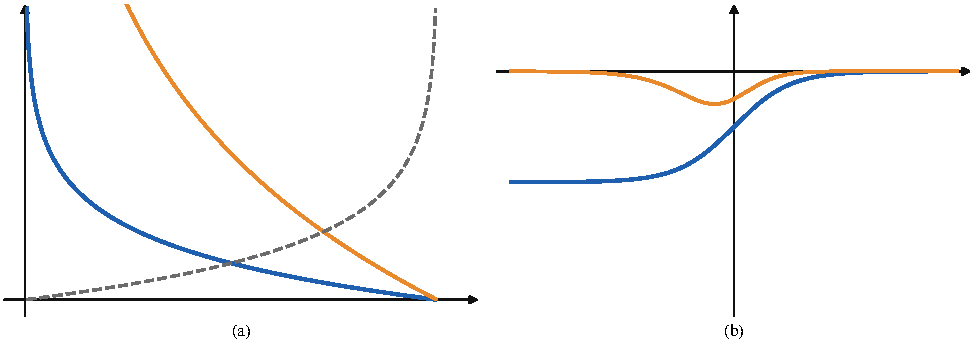
\includegraphics[width=\linewidth]{figures/bce.pdf}
\caption{(a) Strata BCE w funkcji $p$: dla $y=1$ ($-\ln p$, niebieska) i z wagą $\alpha=4$ (pomarańczowa) rośnie do nieskończoności, gdy $p\to0$; dla $y=0$ ($-\ln(1-p)$, szara przerywana)
rośnie, gdy $p\to1$. (b) Gradient po logicie dla $y=1$: BCE (niebieska, $\sigma-1$) pozostaje blisko $-1$ przy dużym błędzie; gradient błędu kwadratowego (pomarańczowa) zanika w nasyceniu.}
\label{rys:bce}
\end{figure*}

\begin{twierdzenie}[BCE uczy prawdziwego prawdopodobieństwa]\label{tw:kalibracja}
Niech etykieta $y\in\{0,1\}$ wypada $1$ z prawdopodobieństwem $q\in(0,1)$. Średnia strata $\Exp[\ell_\alpha(p,y)]=-\alpha q\ln p-(1-q)\ln(1-p)$ jest najmniejsza dla
\begin{equation}
  p^\ast=\frac{\alpha q}{\alpha q+1-q}.
\end{equation}
W szczególności dla $\alpha=1$ jest to $p^\ast=q$.
\end{twierdzenie}
\begin{pomyslDowodu}
Różniczkujemy średnią stratę po $p$, przyrównujemy do zera i sprawdzamy, że to minimum.
\end{pomyslDowodu}
\begin{proof}
Niech $J(p)=-\alpha q\ln p-(1-q)\ln(1-p)$ dla $p\in(0,1)$.
\begin{align*}
J'(p) &= -\frac{\alpha q}{p}+\frac{1-q}{1-p}=0 && \pow{(warunek konieczny)}\\
\Rightarrow\;\alpha q(1-p) &= (1-q)p \;\Rightarrow\; p^\ast=\frac{\alpha q}{\alpha q+1-q}. && \pow{(rozwiązanie względem $p$)}
\end{align*}
Druga pochodna $J''(p)=\alpha q/p^2+(1-q)/(1-p)^2>0$, więc to jedyne minimum. To kończy dowód.
\end{proof}

\begin{naliczbach}
Jeśli w danym półtonie początek nuty występuje w $q=10\%$ przypadków, a waga to $\alpha=4$, model uczony BCE nauczy się mówić $p^\ast=0{,}4/(0{,}4+0{,}9)=0{,}308$, a nie $0{,}1$. Waga zawyża więc prawdopodobieństwa
(rys.~\ref{rys:kalibracja}). Podobnie miękka etykieta $y=0{,}4$ (sąsiednie klatki wokół początku w Gen~6) przy $\alpha=1$ i $q$ interpretowanym jako średnia etykieta daje $p^\ast=0{,}4$: model nie jest karany
za niepewność o jedną klatkę.
\end{naliczbach}

\begin{figure}[ht]
\centering
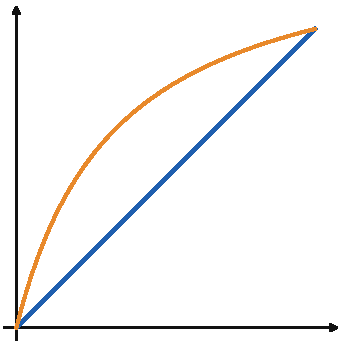
\includegraphics[width=\linewidth]{figures/kalibracja.pdf}
\sidecaption{Optymalne prawdopodobieństwo $p^\ast$ (pion) w zależności od prawdziwej częstości $q$ (poziom) dla wagi $\alpha=1$ (niebieska, leży na przekątnej) i $\alpha=4$ (pomarańczowa, nad przekątną). Waga klasy dodatniej
przesuwa wyjścia sieci w górę; dekoder (rozdział~\ref{rozdz:dekoder}) musi to uwzględnić przez progi dobrane na walidacji. \label{rys:kalibracja}}
\end{figure}

\begin{pulapka}
Wyjścia sieci uczonej z wagą $\alpha>1$ \emph{nie są} prawdziwymi prawdopodobieństwami. Próg $0{,}5$ w dekoderze nie ma wtedy żadnego szczególnego znaczenia; dlatego progi dekodera Gen~6 stroimy osobno (rozdział~\ref{rozdz:dekoder}).
\end{pulapka}

\section{Dlaczego rzadkie etykiety są trudne}

Weźmy prawdziwy przykład: nagranie z rozdziału~\ref{rozdz:hcqt} ($T=243$ klatek, $53$ półtony, $12\,879$ komórek) ma $15$ nut. Mapa początków ma więc tylko $15$ komórek równych $1$ (i $30$ równych $0{,}4$): to $0{,}12\%$ wszystkich.
Sieć, która zawsze odpowiada „zero”, ma niemal idealną dokładność, a zupełnie nie nadaje się do niczego. Dwa środki zaradcze używane w Gen~6: waga $\alpha=4$ dla początków ($\alpha=2$ dla końców) oraz
\emph{inicjalizacja obciążenia} ostatniej warstwy na $-3$ dla początków (i $-2$ dla ramek). Na starcie $\sigma(-3)=0{,}047$, więc strata na komórkę to $-\big[0{,}0012\ln0{,}047+0{,}9988\ln0{,}953\big]=0{,}052$,
a przy $\sigma(0)=0{,}5$ byłoby $0{,}693$: sieć nie musi tracić pierwszych kroków na samo „nauczenie się, że nut jest mało”.

\section{Softmax i tabulatura}

Dla jednej struny w jednej klatce sieć zwraca $21$ logitów (klasa $0$: struna milczy, klasy $1+f$ dla progów $f=0,\dots,19$). Strata to ujemny logarytm prawdopodobieństwa klasy prawdziwej:
$\ell=-\ln\softmax(\vect z)_c=-z_c+\ln\sum_je^{z_j}$. Jej gradient po logitach to $\softmax(\vect z)-\vect e_c$ (analogicznie do tw.~\ref{tw:grad-bce}).

\begin{naliczbach}
Dla trzech klas $\vect z=(2;1;0{,}1)$ i prawdziwej klasy $c=1$ (pierwszej): $\softmax=(0{,}659;\,0{,}242;\,0{,}099)$, strata $-\ln0{,}659=0{,}417$, gradient po logitach $(0{,}659-1;\ 0{,}242;\ 0{,}099)=(-0{,}341;\ 0{,}242;\ 0{,}099)$.
Zwróćmy uwagę: suma gradientu to zero, bo suma softmaksu to $1$ --- podnoszenie jednego logitu odbywa się kosztem pozostałych.
\end{naliczbach}

\section*{Podsumowanie}
\begin{itemize}
\item $\sigma$ zamienia logit na prawdopodobieństwo; softmax robi to dla wielu wykluczających się klas i jest niezmienniczy względem dodania stałej.
\item BCE $=-[y\ln p+(1-y)\ln(1-p)]$; jej gradient po logicie to $\sigma(z)-y$ (tw.~\ref{tw:grad-bce}).
\item BCE jest najmniejsza dla prawdziwej częstości; waga $\alpha$ zawyża wyjścia do $\frac{\alpha q}{\alpha q+1-q}$ (tw.~\ref{tw:kalibracja}).
\item Etykiety początków są rzadkie ($0{,}12\%$ komórek), więc używamy wagi i obciążenia początkowego $-3$.
\item Tabulatura: softmax po $21$ klasach na strunę i strata $-\ln p_{\mathrm{klasa}}$.
\end{itemize}

\begin{sprawdz}
\begin{enumerate}
\item Policz $\sigma(1)$, $\sigma(-1)$ i sprawdź, że sumują się do $1$.
\item Dla $y=1$ policz stratę BCE z $\alpha=1$ oraz $\alpha=2$ przy $p=0{,}3$, a także gradient po logicie w obu przypadkach.
\item Pokaż, że $\softmax(z,0)_1=\sigma(z)$.
\item Przy $q=0{,}05$ i $\alpha=2$ ile wynosi $p^\ast$? Jaką wagę $\alpha$ trzeba wziąć, by $p^\ast=0{,}5$ przy $q=0{,}05$?
\end{enumerate}
\end{sprawdz}

\subsection*{Rozwiązania}
\begin{enumerate}
\item $\sigma(1)=0{,}7311$, $\sigma(-1)=0{,}2689$, suma $1{,}0000$.
\item $\alpha=1$: $-\ln0{,}3=1{,}204$, gradient $0{,}3-1=-0{,}7$. $\alpha=2$: strata $2{,}408$, gradient $-2(1-0{,}3)=-1{,}4$.
\item $\softmax(z,0)_1=e^{z}/(e^{z}+e^{0})=e^{z}/(e^{z}+1)=1/(1+e^{-z})=\sigma(z)$ (dzielimy licznik i mianownik przez $e^{z}$).
\item $p^\ast=2\cdot0{,}05/(0{,}1+0{,}95)=0{,}095$. Z równania $\alpha q=1-q$: $\alpha=(1-q)/q=19$ daje $p^\ast=0{,}5$.
\end{enumerate}

\chapter{Sieć neuronowa: warstwy, konwolucja i normalizacja}\label{rozdz:siec}

\section{Z czego zbudowana jest sieć?}

Sieć neuronowa to złożenie prostych funkcji (rozdział~\ref{rozdz:zapis}); każda z nich ma kilka parametrów, które dobieramy gradientem
(rozdział~\ref{rozdz:pochodne}). Model Gen~6 używa pięciu rodzajów cegiełek: warstwy liniowej (rozdział~\ref{rozdz:wektory}), funkcji nieliniowej GELU,
konwolucji, normalizacji warstwy i połączeń resztkowych. Poznajmy je po kolei, ze sprawdzeniem na małych liczbach.

Po tym rozdziale umiesz: (i)~policzyć GELU i konwolucję jednowymiarową ręcznie, (ii)~policzyć liczbę parametrów konwolucji,
(iii)~wyznaczyć pole widzenia stosu konwolucji z dylatacją, (iv)~uzasadnić własności LayerNorm i połączenia resztkowego.

\section{Nieliniowość: po co i jaka}

Z twierdzenia~\ref{tw:mnozenie} wiemy, że dwie warstwy liniowe to jedna warstwa liniowa. Żeby głębokość coś dawała, między warstwami wstawiamy funkcję nieliniową działającą na każdą liczbę osobno.

\haslo{GELU}
\begin{definicja}[GELU]\label{def:gelu}
Niech $\Phi(z)=\tfrac12\big(1+\operatorname{erf}(z/\sqrt2)\big)$ będzie dystrybuantą rozkładu normalnego $N(0,1)$. Funkcja
$\GELU(z)=z\,\Phi(z)$ „bramkuje” wejście: mnoży je przez prawdopodobieństwo, że losowa liczba $N(0,1)$ jest mniejsza od $z$.
Dla porównania $\ReLU(z)=\max(0,z)$.
\end{definicja}

\begin{przyklad}\label{prz:gelu}
$\GELU(2)=2\cdot0{,}9772=1{,}9545$, $\GELU(1)=0{,}8413$, $\GELU(0)=0$, $\GELU(-1)=-0{,}1587$, $\GELU(-3)=-0{,}0040$.
Dla dużych dodatnich $z$ funkcja zachowuje się jak $z$, dla dużych ujemnych dąży do zera; w okolicy zera jest gładka (rys.~\ref{rys:gelu}).
\end{przyklad}

\begin{figure}[ht]
\centering
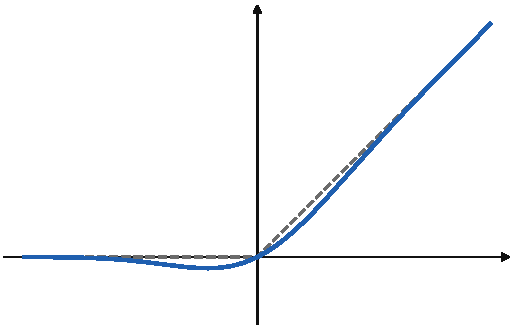
\includegraphics[width=\linewidth]{figures/gelu.pdf}
\sidecaption{GELU (niebieska) i ReLU (szara przerywana). GELU jest gładką wersją ReLU: w odróżnieniu od niego ma niewielką ujemną „zatokę” (minimum ok.\ $-0{,}17$) i nie ma ostrego załamania w zerze,
więc ma pochodną wszędzie. \label{rys:gelu}}
\end{figure}

\begin{intuicja}
ReLU wycina wszystko ujemne. GELU robi to łagodnie: małe ujemne wartości są tylko osłabiane. Przez to pochodna zmienia się płynnie i sieć uczy się stabilniej. Sam kształt nie jest świętością --- ważne jest, by funkcja była nieliniowa.
\end{intuicja}

\section{Konwolucja}

Warstwa liniowa łączy każde wejście z każdym wyjściem. Dla sygnałów, w których ten sam wzorzec może wystąpić w różnych miejscach (nuta w dowolnej klatce, wzorzec alikwotów w dowolnej wysokości), lepsza jest warstwa, która
\emph{używa tych samych wag w każdym miejscu}.

\haslo{konwolucja}
\begin{definicja}[Konwolucja jednowymiarowa]\label{def:konwolucja}
Dla sygnału $x[t]$ i \emph{jądra} $w[-r],\dots,w[r]$ (długość $k=2r+1$) wynik konwolucji z krokiem $1$ i dopełnieniem zerami to
\begin{equation}
  y[t]=b+\sum_{j=-r}^{r}w[j]\,x[t+j],
\end{equation}
przy czym $x[s]=0$ poza zakresem. \emph{Dylatacja} $d$ rozstawia próbki jądra co $d$: $y[t]=b+\sum_j w[j]\,x[t+dj]$.
\emph{Krok} (stride) $s$ oblicza wynik tylko co $s$-te $t$.
\end{definicja}

\begin{przyklad}\label{prz:konwolucja}
Sygnał $x=(1,2,3,4,5,6)$, jądro $w=(1,0,-1)$ (dla $j=-1,0,1$), $b=0$: $y[t]=x[t-1]-x[t+1]$. Wynik: $y=(-2,-2,-2,-2,-2,\,5)$.
Różnica „poprzedni minus następny” wynosi $-2$ wszędzie, gdzie sygnał rośnie liniowo; ostatnia wartość $5=x[5]-0$ pochodzi z dopełnienia zerem, które
udaje, że za końcem jest $x=0$. Takie jądro wykrywa nachylenie sygnału, czyli działa jak pochodna.
\end{przyklad}

W obrazach i widmach (dwa wymiary: czas i bin) jądro ma kształt $k_t\times k_p$ i przesuwa się w obu osiach. Jeśli każde z $C_\mathrm{we}$ kanałów wejściowych ma osobne jądro, a wyniki sumujemy do $C_\mathrm{wy}$ kanałów:

\begin{twierdzenie}[Liczba parametrów konwolucji]\label{tw:param-konw}
Konwolucja $k_t\times k_p$ z $C_\mathrm{we}$ kanałów do $C_\mathrm{wy}$ kanałów ma $C_\mathrm{we}\,C_\mathrm{wy}\,k_tk_p+C_\mathrm{wy}$ parametrów, a konwolucja \emph{głębokościowa} (osobne jądro dla każdego kanału, $C_\mathrm{we}=C_\mathrm{wy}=C$)
ma $C\,k_tk_p+C$ parametrów. Liczba ta \emph{nie zależy} od długości sygnału.
\end{twierdzenie}
\begin{pomyslDowodu}
Każdy z $C_\mathrm{wy}$ kanałów wyjściowych ma po jednym jądrze $k_t\times k_p$ dla każdego kanału wejściowego i jedno obciążenie.
\end{pomyslDowodu}
\begin{proof}
Jedno jądro ma $k_tk_p$ liczb. Kanał wyjściowy sumuje wkłady wszystkich kanałów wejściowych, więc ma $C_\mathrm{we}$ jąder i jedno obciążenie $b$.
\begin{align*}
\#\text{parametrów} &= C_\mathrm{wy}\cdot\big(C_\mathrm{we}\cdot k_tk_p+1\big) && \pow{(po kanale wyjściowym)}\\
 &= C_\mathrm{we}C_\mathrm{wy}k_tk_p+C_\mathrm{wy}. && \pow{(rozdzielność)}
\end{align*}
W wersji głębokościowej każdy kanał ma tylko jedno jądro (dla samego siebie): $C(k_tk_p+1)$. Wagi są te same dla każdego położenia, więc liczba parametrów nie rośnie z długością sygnału. To kończy dowód.
\end{proof}

\begin{naliczbach}
Trzon Gen~6: konwolucja $3\times7$ z $9$ kanałów (HCQT) do $48$: $9\cdot48\cdot21+48=9120$. Konwolucja głębokościowa $1\times5$ na $48$ kanałach: $48\cdot5+48=288$.
Konwolucja czasowa $3\times1$, $48\to48$: $48\cdot48\cdot3+48=6960$. Konwolucja $1\times1$ ($336\to48$): $336\cdot48+48=16\,176$ (to warstwa liniowa działająca w każdym miejscu osobno).
\end{naliczbach}

\begin{twierdzenie}[Konwolucja jest równoważna przesunięciom]\label{tw:rownowaznosc}
Niech $(Tx)[t]=x[t-s]$ będzie przesunięciem sygnału o $s$ w czasie. Konwolucja $C$ (bez dopełnienia, w nieskończonym sygnale) spełnia $C(Tx)=T(Cx)$.
\end{twierdzenie}
\begin{pomyslDowodu}
Wstawiamy przesunięty sygnał do definicji i przesuwamy indeks.
\end{pomyslDowodu}
\begin{proof}
\begin{align*}
(C(Tx))[t] &= b+\sum_j w[j]\,(Tx)[t+j] && \pow{(def.~\ref{def:konwolucja})}\\
 &= b+\sum_j w[j]\,x[t+j-s] && \pow{(def.\ $T$)}\\
 &= (Cx)[t-s]=(T(Cx))[t]. && \pow{(def.\ $C$ w punkcie $t-s$)}
\end{align*}
Przesunięcie wejścia o $s$ klatek przesuwa wynik o $s$ klatek, a niczego innego nie zmienia: ta sama nuta w innym momencie daje ten sam wzorzec odpowiedzi. To kończy dowód.
\end{proof}

W praktyce to właśnie dlatego konwolucja po osi binów (na osi logarytmicznej, rozdział~\ref{rozdz:alikwoty}) wykrywa ten sam wzorzec nuty o dowolnej wysokości.

\haslo{pole widzenia}
\begin{twierdzenie}[Pole widzenia]\label{tw:pole-widzenia}
Stos $n$ konwolucji w czasie z jądrami długości $k_i=2r_i+1$ i dylatacjami $d_i$ ma \emph{pole widzenia} (liczbę klatek wejścia z każdej strony, które wpływają na jedną klatkę wyjścia)
$R=\sum_{i=1}^{n}d_ir_i$.
\end{twierdzenie}
\begin{pomyslDowodu}
Indukcja po liczbie warstw: każda nowa warstwa rozszerza zbiór zależności o $d_ir_i$ klatek z każdej strony.
\end{pomyslDowodu}
\begin{proof}
Dla $n=1$: wyjście w klatce $t$ zależy od wejść w $t+d_1j$, $|j|\le r_1$, czyli od klatek odległych najwyżej o $d_1r_1$. Załóżmy, że wyjście warstwy $n-1$ w klatce $u$ zależy od wejść odległych najwyżej o $R_{n-1}$.
Wyjście warstwy $n$ w klatce $t$ zależy od wyjść warstwy $n-1$ w $u=t+d_nj$, $|j|\le r_n$, a każde z nich od wejść odległych o co najwyżej $R_{n-1}$ od $u$. Najdalsza zależność od $t$ to
\begin{align*}
|u-t|+R_{n-1}\le d_nr_n+R_{n-1}=R_n && \pow{(nierówność trójkąta)}
\end{align*}
i ta odległość jest osiągana (dla $j=\pm r_n$ i skrajnej zależności wcześniejszej, gdy odpowiednie wagi są niezerowe). Zatem $R=\sum d_ir_i$. To kończy dowód.
\end{proof}

\begin{figure*}[ht]
\centering
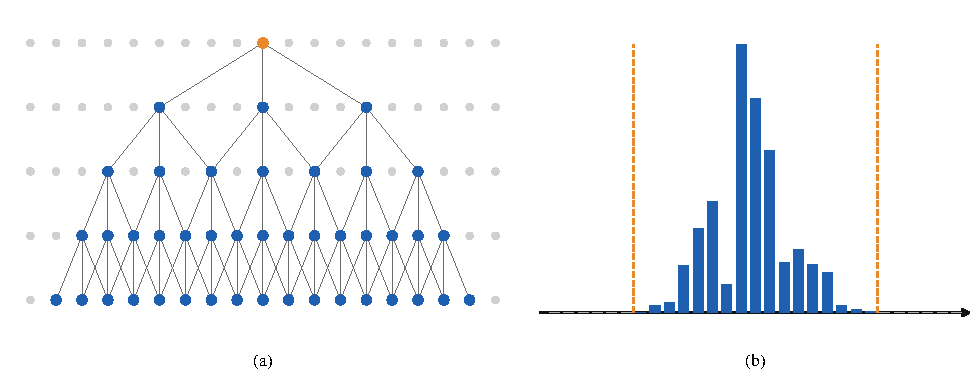
\includegraphics[width=\linewidth]{figures/pole-widzenia.pdf}
\caption{(a) Schemat czterech konwolucji czasowych z jądrem $3$ i dylatacjami $1$ (trzon), $1,2,4$ (od wejścia na dole do wyjścia na górze): pomarańczowa kropka to jedna klatka wyjścia, niebieskie to klatki wejścia, od których zależy
(zasięg $\pm8=1+1+2+4$). Z dylatacją pole widzenia rośnie wykładniczo, a nie liniowo, przy tej samej liczbie parametrów.
(b) Pomiar: moduł gradientu jednej wartości wyjścia po wejściu w funkcji odległości w klatkach dla stosu z trzonem $3\times7$ i trzema blokami z dylatacjami $1,2,4$ (losowe wagi, PyTorch): gradient jest niezerowy dokładnie dla $|t|\le8=1+(1+2+4)$ (niebieskie) i zerowy poza (szare).}
\label{rys:pole-widzenia}
\end{figure*}

\begin{przyklad}[Pole widzenia bloków Gen~6]\label{prz:pole-gen6}
Trzon ma jądro $3$ w czasie ($r=1$, $d=1$) i trzy bloki mają jądro $3$ z $d=1,2,4$: $R=1+(1+2+4)=8$ klatek, czyli $\pm8\cdot23{,}2\ms=\pm186\ms$. Pomiar na prawdziwym stosie (rys.~\ref{rys:pole-widzenia}b) potwierdza $\pm8$.
\end{przyklad}

\section{Normalizacja warstwy i połączenia resztkowe}

\haslo{LayerNorm}
\begin{definicja}[LayerNorm]\label{def:ln}
Dla wektora $\vect z\in\R^D$ niech $\mu=\frac1D\sum z_i$ i $\sigma^2=\frac1D\sum(z_i-\mu)^2$. \emph{Normalizacja warstwy} to
$\LN(\vect z)_i=\gamma_i\,\dfrac{z_i-\mu}{\sqrt{\sigma^2+\varepsilon}}+\beta_i$, gdzie $\gamma,\beta\in\R^D$ są uczone ($\gamma=1,\beta=0$ na starcie), a $\varepsilon=10^{-5}$ chroni przed dzieleniem przez zero.
\end{definicja}

\begin{przyklad}\label{prz:ln}
Dla $\vect z=(1,2,3,6)$: $\mu=3$, $\sigma^2=(4+1+0+9)/4=3{,}5$, $\sigma=1{,}871$. Wynik (przy $\gamma=1$, $\beta=0$, $\varepsilon\to0$): $(-1{,}069;\,-0{,}535;\,0;\,1{,}604)$ ma średnią $0$ i wariancję $1$.
\end{przyklad}

\begin{twierdzenie}[Niezmienniczość LayerNorm]\label{tw:ln}
Dla $\varepsilon=0$, $\gamma=1$, $\beta=0$ i dowolnych $a>0$, $c\in\R$: $\LN(a\vect z+c\vect 1)=\LN(\vect z)$.
\end{twierdzenie}
\begin{pomyslDowodu}
Skalowanie i przesunięcie zmieniają średnią i odchylenie dokładnie w taki sposób, że licznik i mianownik skracają się.
\end{pomyslDowodu}
\begin{proof}
Dla $\vect z'=a\vect z+c\vect1$: $\mu'=a\mu+c$ oraz
\begin{align*}
\sigma'^2 &= \frac1D\sum(az_i+c-a\mu-c)^2=a^2\sigma^2 && \pow{(wyrazy $c$ się znoszą)}\\
\frac{z'_i-\mu'}{\sigma'} &= \frac{a(z_i-\mu)}{a\sigma}=\frac{z_i-\mu}{\sigma}. && \pow{($a>0$, więc $\sqrt{a^2}=a$)}
\end{align*}
Obie strony równości są więc identyczne. To kończy dowód.
\end{proof}

W zwykłym języku: LayerNorm usuwa informację o skali i przesunięciu wektora cech i zostawia tylko jego „kształt”; wymusza to stabilny rozmiar liczb płynących przez sieć. Wady: nie działa na wektorach stałych ($\sigma=0$; stąd $\varepsilon$).

\haslo{połączenie resztkowe}
\begin{definicja}[Połączenie resztkowe]\label{def:residual}
Blok z połączeniem resztkowym liczy $\vect y=\vect x+F(\vect x)$, gdzie $F$ to dowolna warstwa lub kilka warstw (rys.~\ref{rys:blok}).
\end{definicja}

\begin{twierdzenie}[Gradient przez połączenie resztkowe]\label{tw:residual}
Dla $\vect y=\vect x+F(\vect x)$ macierz pochodnych (jakobian) to $\dfrac{\partial\vect y}{\partial\vect x}=I+\dfrac{\partial F}{\partial\vect x}$. Dla stosu $L$ takich bloków
\begin{equation}
  \frac{\partial\vect y_L}{\partial\vect x}=\prod_{l=1}^{L}\big(I+J_l\big)=I+\sum_{l}J_l+(\text{wyrazy wyższych rzędów w }J).
\end{equation}
\end{twierdzenie}
\begin{pomyslDowodu}
Pochodna sumy to suma pochodnych, a pochodna $\vect x$ po $\vect x$ to macierz jednostkowa; dla stosu mnożymy jakobiany (reguła łańcuchowa).
\end{pomyslDowodu}
\begin{proof}
Z liniowości pochodnej $\partial(\vect x+F(\vect x))/\partial\vect x=\partial\vect x/\partial\vect x+\partial F/\partial\vect x=I+J$. Dla stosu reguła łańcuchowa daje iloczyn jakobianów kolejnych bloków. Rozwijając iloczyn $(I+J_L)\cdots(I+J_1)$ otrzymujemy $I$ (wybór składnika $I$ z każdego nawiasu), plus $J_l$ (jeden nawias daje $J$), plus iloczyny dwóch i więcej $J$. Człon $I$ nie zależy od $F$. To kończy dowód.
\end{proof}

W zwykłym języku: nawet jeśli $F$ ma bardzo małe pochodne, sygnał uczący przepływa przez „autostradę” $I$ i nie znika. Dzięki temu można ułożyć wiele bloków bez ryzyka, że gradient wygaśnie po drodze.

\begin{naliczbach}
Dla skalarnej $F(x)=0{,}01x$ i $L=50$ bloków: z połączeniem $\prod(1+0{,}01)=1{,}01^{50}=1{,}645$, bez niego $\prod0{,}01=10^{-100}$. Gradient bez autostrady byłby praktycznie zerem.
\end{naliczbach}

\begin{figure}[ht]
\centering
\begin{tikzpicture}[>=Stealth,node distance=6mm]
  \node[blok,minimum width=14mm] (x) {$\vect x$};
  \node[blok,minimum width=16mm,right=of x] (ln) {$\LN$};
  \node[blok,minimum width=16mm,right=of ln] (f) {$F$};
  \node[blok,minimum width=14mm,right=of f] (drop) {$\Drop$};
  \node[wezel,right=8mm of drop] (plus) {$+$};
  \node[right=7mm of plus] (y) {$\vect y$};
  \draw[wektor] (x)--(ln); \draw[wektor] (ln)--(f); \draw[wektor] (f)--(drop); \draw[wektor] (drop)--(plus); \draw[wektor] (plus)--(y);
  \draw[wektor] (x.north) -- ++(0,6mm) -| (plus.north);
\end{tikzpicture}
\sidecaption{Blok resztkowy typu „pre-norm”, jak w warstwach Gen~6: wejście $\vect x$ jest normalizowane (LN), przechodzi przez $F$ (konwolucja albo uwaga) i dropout, a następnie dodawane do niezmienionego $\vect x$ (górna ścieżka). Wynik: $\vect y=\vect x+\Drop(F(\LN(\vect x)))$. \label{rys:blok}}
\end{figure}

\haslo{dropout}
\begin{definicja}[Dropout]\label{def:dropout}
W uczeniu \emph{dropout} z prawdopodobieństwem $\rho$ zeruje każdą współrzędną wektora, a pozostałe mnoży przez $\frac1{1-\rho}$. Przy wnioskowaniu nie robi nic.
\end{definicja}

\begin{wniosek}[Dropout nie zmienia średniej]\label{wn:dropout}
Dla $\vect x$ ustalonego, $\Exp[\Drop(\vect x)]=\vect x$.
\end{wniosek}
\begin{proof}
Dla jednej współrzędnej $x_i$ wynik wynosi $0$ z prawdopodobieństwem $\rho$ i $x_i/(1-\rho)$ z prawdopodobieństwem $1-\rho$. Stąd
\begin{align*}
\Exp[\Drop(x_i)] &= \rho\cdot0+(1-\rho)\cdot\frac{x_i}{1-\rho}=x_i. && \pow{(definicja wartości oczekiwanej)}
\end{align*}
Skalowanie przez $\frac{1}{1-\rho}$ sprawia, że przy wnioskowaniu (bez dropoutu) liczby mają ten sam rząd wielkości co w uczeniu. Gen~6 używa $\rho=0{,}1$. To kończy dowód.
\end{proof}

\begin{pulapka}
LayerNorm i dropout zachowują się inaczej w uczeniu i wnioskowaniu (dropout) lub zależą od wymiaru (LayerNorm liczy po cechach jednego punktu, nie po paczce). Błąd typowy: zapomnieć wywołać \texttt{model.eval()} przed przewidywaniem; sieć wciąż losowo zeruje cechy i wyniki są inne przy każdym uruchomieniu.
\end{pulapka}

\section*{Podsumowanie}
\begin{itemize}
\item Między warstwami liniowymi stawiamy nieliniowość GELU $=z\Phi(z)$.
\item Konwolucja używa tych samych wag w każdym miejscu; liczba parametrów to $C_\mathrm{we}C_\mathrm{wy}k_tk_p+C_\mathrm{wy}$ i nie zależy od długości sygnału (tw.~\ref{tw:param-konw}); jest równoważna przesunięciom (tw.~\ref{tw:rownowaznosc}).
\item Pole widzenia stosu konwolucji: $R=\sum d_ir_i$ (tw.~\ref{tw:pole-widzenia}); dla bloków Gen~6 $R=8$ klatek.
\item LayerNorm usuwa skalę i przesunięcie wektora cech (tw.~\ref{tw:ln}).
\item Połączenie resztkowe $\vect x+F(\vect x)$ zachowuje gradient (tw.~\ref{tw:residual}); dropout nie zmienia średniej (wn.~\ref{wn:dropout}).
\end{itemize}

\begin{sprawdz}
\begin{enumerate}
\item Policz konwolucję $x=(2,0,1,3)$ z jądrem $w=(1,2,1)$ (dla $j=-1,0,1$, $b=0$) i dopełnieniem zerami.
\item Ile parametrów ma konwolucja $5\times5$ z $16$ do $32$ kanałów? A głębokościowa $5\times5$ na $32$ kanałach?
\item Stos czterech konwolucji z jądrem $3$ i dylatacjami $1,2,4,8$. Jakie jest pole widzenia? Ile wynosiłoby bez dylatacji?
\item Policz $\LN(\vect z)$ dla $\vect z=(4,4,8)$ ($\gamma=1,\beta=0,\varepsilon\to0$).
\end{enumerate}
\end{sprawdz}

\subsection*{Rozwiązania}
\begin{enumerate}
\item $y[0]=1\cdot0+2\cdot2+1\cdot0=4$ (bo $x[-1]=0$); $y[1]=1\cdot2+2\cdot0+1\cdot1=3$; $y[2]=1\cdot0+2\cdot1+1\cdot3=5$; $y[3]=1\cdot1+2\cdot3+1\cdot0=7$. Wynik $(4,3,5,7)$.
\item $16\cdot32\cdot25+32=12\,832$; głębokościowa: $32\cdot25+32=832$.
\item $R=1+2+4+8=15$ klatek z każdej strony; bez dylatacji $R=4$.
\item $\mu=16/3=5{,}333$; $\sigma^2=\frac13\big(2\cdot1{,}778+7{,}111\big)=3{,}556$, $\sigma=1{,}886$. Wynik: $(-0{,}707;\,-0{,}707;\,1{,}414)$.
\end{enumerate}

\chapter{Uwaga (attention)}\label{rozdz:uwaga}

\section{Czemu konwolucja nie wystarcza?}

Konwolucja patrzy na stały, mały sąsiad (rozdział~\ref{rozdz:siec}). Tymczasem żeby ocenić, czy w danej klatce gra E3, sieć powinna
sprawdzić, czy gra też E2 (oktawę niżej, której alikwoty zlewają się z E3) i czy ta sama nuta trwała w poprzednich klatkach. To są
\emph{dalekie} zależności, a ich siła zależy od treści: oktawa jest ważna zawsze, ale tylko wtedy, gdy dwie nuty rzeczywiście grają razem.
Mechanizm, który wybiera, na co patrzeć, na podstawie treści, nazywamy \emph{uwagą}.

Po tym rozdziale umiesz: (i)~policzyć uwagę dla kilku elementów ręcznie, (ii)~uzasadnić, że wynik jest średnią ważoną wartości,
(iii)~wyjaśnić, skąd się bierze dzielenie przez $\sqrt{d}$, (iv)~policzyć liczbę parametrów warstwy uwagi i wskazać, jak nadać jej wiedzę o położeniu.

\section{Uwaga pojedynczego zapytania}

Każdy element sekwencji dostaje trzy wektory: \emph{zapytanie} $\vect q$ („czego szukam”), \emph{klucz} $\vect k$ („co oferuję”) i \emph{wartość} $\vect v$ („co przekazuję, gdy mnie wybierzesz”).
Powstają z wektora cech $\vect h$ przez trzy macierze: $\vect q=W_Q\vect h$, $\vect k=W_K\vect h$, $\vect v=W_V\vect h$ (rozdział~\ref{rozdz:wektory}).

\haslo{uwaga}
\begin{definicja}[Uwaga skalowana iloczynem skalarnym]\label{def:uwaga}
Dla zapytania $\vect q\in\R^d$, kluczy $\vect k_1,\dots,\vect k_n\in\R^d$ i wartości $\vect v_1,\dots,\vect v_n\in\R^{d_v}$ oraz opcjonalnych \emph{premii} $b_j\in\R$:
\begin{equation}
  s_j=\frac{\ip{\vect q}{\vect k_j}}{\sqrt d}+b_j,\qquad
  \alpha_j=\softmax(s)_j,\qquad
  \operatorname{Attn}(\vect q)=\sum_{j=1}^{n}\alpha_j\,\vect v_j .
\end{equation}
Liczby $\alpha_j$ nazywamy \emph{wagami uwagi}.
\end{definicja}

\begin{przyklad}[Trzy elementy, policzone ręcznie]\label{prz:uwaga}
Niech $d=2$, $\vect q=(1,0)$, klucze $\vect k_1=(1,0)$, $\vect k_2=(0,1)$, $\vect k_3=(1,1)$, wartości $\vect v_1=(1,0)$, $\vect v_2=(0,1)$, $\vect v_3=(2,2)$, premie $b=0$.
Wyniki $\ip{\vect q}{\vect k_j}=(1,0,1)$, dzielone przez $\sqrt2$: $s=(0{,}707;\,0;\,0{,}707)$. Wykładniki: $(2{,}028;\,1;\,2{,}028)$, suma $5{,}056$, wagi $\alpha=(0{,}401;\,0{,}198;\,0{,}401)$.
Wynik: $0{,}401\cdot(1,0)+0{,}198\cdot(0,1)+0{,}401\cdot(2,2)=(1{,}203;\;1{,}000)$.
Zapytanie $(1,0)$ „pasuje” do kluczy $1$ i $3$ (oba mają pierwszą współrzędną $1$), więc one dominują w wyniku. Gdyby klucz $3$ dostał premię $b_3=-1$, jego waga spadłaby do $0{,}198$ i wynik zmieniłby się na $(0{,}933;\,0{,}660)$.
\end{przyklad}

\begin{intuicja}
Uwaga to miękkie wyszukiwanie w słowniku: zapytanie porównujemy ze wszystkimi kluczami (iloczyn skalarny = podobieństwo), zamieniamy podobieństwa na wagi (softmax) i zwracamy średnią wartości ważoną tymi wagami.
Zamiast jednego wyniku „dokładnie to hasło” dostajemy mieszankę wszystkich, z naciskiem na najlepiej pasujące.
\end{intuicja}

\begin{twierdzenie}[Wynik uwagi to średnia ważona]\label{tw:uwaga-wypukla}
Wagi spełniają $\alpha_j>0$ i $\sum_j\alpha_j=1$, więc $\operatorname{Attn}(\vect q)$ leży w otoczce wypukłej wartości $\vect v_1,\dots,\vect v_n$: dla każdej współrzędnej $l$,
$\min_jv_{j,l}\le\operatorname{Attn}(\vect q)_l\le\max_jv_{j,l}$.
\end{twierdzenie}
\begin{pomyslDowodu}
Wagi są wynikiem softmaksa (tw.~\ref{tw:softmax}); średnia ważona dodatnimi wagami o sumie $1$ nie wychodzi poza zakres wartości.
\end{pomyslDowodu}
\begin{proof}
Z tw.~\ref{tw:softmax}(a): $\alpha_j>0$ i $\sum\alpha_j=1$. Niech $m=\min_jv_{j,l}$, $M=\max_jv_{j,l}$.
\begin{align*}
\operatorname{Attn}(\vect q)_l &= \sum_j\alpha_jv_{j,l}\le\sum_j\alpha_jM=M && \pow{($\alpha_j>0$, $v_{j,l}\le M$)}\\
\operatorname{Attn}(\vect q)_l &\ge \sum_j\alpha_jm=m. && \pow{(analogicznie)}
\end{align*}
Wynik leży więc między skrajnymi wartościami. Warstwa uwagi nie „wymyśla” nowych wartości spoza zakresu, tylko je miesza; to ona wybiera, w jakich proporcjach. To kończy dowód.
\end{proof}

\section{Dlaczego dzielimy przez $\sqrt{d}$}

\begin{twierdzenie}[Wariancja iloczynu skalarnego]\label{tw:wariancja}
Jeśli współrzędne $q_i,k_i$ są niezależnymi zmiennymi losowymi o średniej $0$ i wariancji $1$, to $\Exp[\ip{\vect q}{\vect k}]=0$ i $\Var(\ip{\vect q}{\vect k})=d$.
Zatem $\ip{\vect q}{\vect k}/\sqrt d$ ma wariancję $1$ niezależnie od $d$.
\end{twierdzenie}
\begin{pomyslDowodu}
Iloczyn skalarny to suma $d$ niezależnych składników $q_ik_i$, z których każdy ma średnią $0$ i wariancję $1$; wariancje niezależnych składników się dodają.
\end{pomyslDowodu}
\begin{proof}
Dla jednego składnika, z niezależności $q_i$ i $k_i$:
\begin{align*}
\Exp[q_ik_i] &= \Exp[q_i]\,\Exp[k_i]=0, && \pow{(niezależność)}\\
\Var(q_ik_i) &= \Exp[q_i^2k_i^2]=\Exp[q_i^2]\,\Exp[k_i^2]=1\cdot1=1. && \pow{(średnia $0$, więc $\Var=\Exp[\cdot^2]$)}
\end{align*}
Składniki są niezależne, więc wariancja sumy to suma wariancji: $\Var\big(\sum_iq_ik_i\big)=d$. Dzielenie przez $\sqrt d$ dzieli wariancję przez $d$ (stała wychodzi do kwadratu). To kończy dowód.
\end{proof}

W zwykłym języku: im dłuższe wektory, tym większe losowe wyniki iloczynów. Duże wyniki wpychają softmax w nasycenie (jedna waga bliska $1$, reszta $\approx0$), gdzie jego gradient zanika. Skalowanie utrzymuje wyniki w rozsądnym zakresie
(rys.~\ref{rys:uwaga}c: pomarańczowy rozrzut rośnie jak $\sqrt d$, niebieski, po skalowaniu, jest stały).

\section{Uwaga dla całej sekwencji i premie położenia}

Gdy każdy z $n$ elementów jest też zapytaniem, wszystko zapisujemy macierzowo: $Q,K,V\in\R^{n\times d}$ (wiersze to wektory), $\operatorname{Attn}(Q,K,V)=\softmax\!\big(QK^{\top}/\sqrt d+B\big)V$, gdzie softmax działa na każdy wiersz,
a $B\in\R^{n\times n}$ to macierz premii. Wynikiem jest nowy zestaw $n$ wektorów.

\begin{twierdzenie}[Bez premii uwaga nie zna kolejności]\label{tw:permutacje}
Niech $P$ będzie macierzą permutacji. Dla $B=0$: $\operatorname{Attn}(PQ,PK,PV)=P\,\operatorname{Attn}(Q,K,V)$.
\end{twierdzenie}
\begin{pomyslDowodu}
Permutacja wierszy $Q,K$ permutuje wiersze i kolumny macierzy wyników w ten sam sposób; softmax po wierszach tego nie zauważa.
\end{pomyslDowodu}
\begin{proof}
$(PQ)(PK)^\top=PQK^\top P^\top$, więc macierz wyników $S$ zamienia się w $PSP^\top$: wiersze i kolumny są przetasowane tak samo. Softmax liczony po wierszach przestawia kolumny wewnątrz wiersza bez zmiany wag, a $P$ przestawia wiersze:
$\softmax(PSP^\top)=P\,\softmax(S)\,P^\top$. Stąd
\begin{align*}
\operatorname{Attn}(PQ,PK,PV) &= P\,\softmax(S)\,P^\top P V && \pow{($P^\top P=I$)}\\
 &= P\,\operatorname{Attn}(Q,K,V). && \pow{(def.)}
\end{align*}
Przetasowanie wejścia tylko przetasowuje wyjście. To kończy dowód.
\end{proof}

W zwykłym języku: samo „co” nie mówi „gdzie”. Gdyby klatki wymieszać, uwaga nie zauważy. Dlatego dodajemy \emph{premię zależną od odległości} $b_{j-i}$ (wyuczoną liczbę dla każdej różnicy położeń): sieć może się nauczyć, że odległość $12$ półtonów (oktawa) jest szczególnie ważna,
albo że klatka sprzed $0{,}5$ s ma inną wagę niż sąsiednia. Niektóre pary można też zablokować, ustawiając $b=-\infty$ (waga wtedy dokładnie $0$): tak powstaje \emph{okno} $\abs{j-i}\le W$ (rys.~\ref{rys:uwaga}b), które w Gen~6 ma $W=43$ klatki ($\approx1$ s) i kosztuje $O(n(2W+1))$ zamiast $O(n^2)$.

\begin{figure*}[ht]
\centering
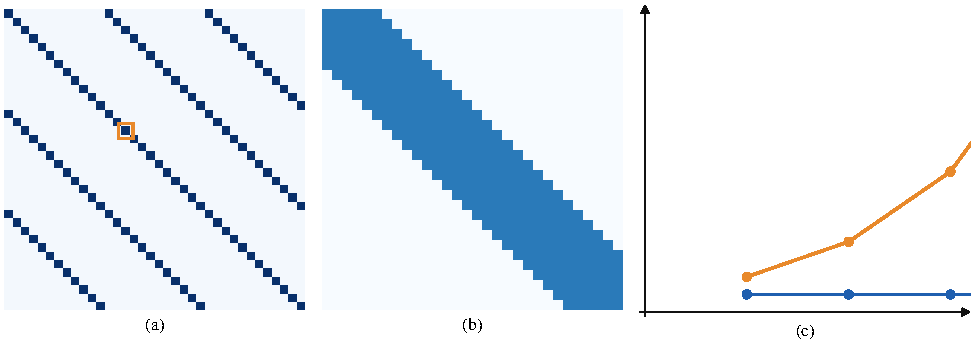
\includegraphics[width=\linewidth]{figures/uwaga.pdf}
\caption{(a) Zabawka: $36$ półtonów, a zapytanie i klucz to wskazanie klasy wysokości $(i\bmod12)$. Każdy wiersz macierzy wag $\alpha$ ma ciemne pola tylko dla tej samej klasy, czyli co $12$ półtonów: wysokość $14$ (pomarańczowa ramka)
patrzy na $2$, $14$ i $26$ --- uwaga potrafi „zobaczyć” oktawy. (b) Maska okna $\abs{t-u}\le5$ dla $30$ klatek: tylko pasmo wokół przekątnej ma niezerowe wagi. (c) Odchylenie standardowe $\ip{\vect q}{\vect k}$ dla wymiarów $d=4,16,64,256$ (oś pozioma $\log_2d$):
bez skalowania (pomarańczowa) rośnie jak $\sqrt d$, po podzieleniu przez $\sqrt d$ (niebieska) jest równe $1$. Obliczone z $10^5$ losowych par.}
\label{rys:uwaga}
\end{figure*}

\begin{figure}[ht]
\centering
\begin{tikzpicture}[>=Stealth,node distance=5mm,font=\small]
  \node[blok,minimum width=9mm] (h) {$H$};
  \node[blok,above right=2mm and 9mm of h,minimum width=9mm] (q) {$Q$};
  \node[blok,right=9mm of h,minimum width=9mm] (k) {$K$};
  \node[blok,below right=2mm and 9mm of h,minimum width=9mm] (v) {$V$};
  \node[blok,right=9mm of k,minimum width=16mm] (s) {$\softmax\!\big(\tfrac{QK^\top}{\sqrt d}+B\big)$};
  \node[blok,right=9mm of s,minimum width=9mm] (o) {$\times V$};
  \draw[wektor] (h)--(q); \draw[wektor] (h)--(k); \draw[wektor] (h)--(v);
  \draw[wektor] (q.east)--++(2mm,0)|-(s.west); \draw[wektor] (k)--(s);
  \draw[wektor] (s)--(o); \draw[wektor] (v.east)--++(2mm,0) -| ([xshift=3mm]o.south);
\end{tikzpicture}
\sidecaption{Przepływ danych jednej głowicy uwagi. Wektory cech $H\in\R^{n\times D}$ są rzutowane na $Q,K,V\in\R^{n\times d_h}$; iloczyny $QK^\top\in\R^{n\times n}$ (wyniki dopasowania), dzielone przez $\sqrt{d}$ i powiększone o premie $B$, przechodzą przez softmax
wiersz po wierszu; powstałe wagi mnożą $V$ i dają wyjście $n\times d_h$. \label{rys:uwaga-schemat}}
\end{figure}

\section{Wiele głowic i liczba parametrów}

Jedna uwaga potrafi śledzić jedną zależność naraz. \emph{Wielogłowicowa} uwaga dzieli wektor $D$-wymiarowy na $n_h$ części po $d_h=D/n_h$, w każdej liczy osobną uwagę (osobne $W_Q,W_K,W_V$ i osobne premie), skleja wyniki i mnoży przez $W_O$.
W Gen~6: $D=64$, $n_h=4$, $d_h=16$.

\begin{naliczbach}
Macierz $W_{QKV}\colon64\to192$ (trzy macierze naraz) ma $64\cdot192+192=12\,480$ parametrów; $W_O\colon64\to64$ ma $64\cdot64+64=4160$. Premie czasowe: $n_h(2W+1)=4\cdot87=348$; premie między wysokościami: $n_h(2S-1)=4\cdot105=420$
(dla $S=53$). Uwaga w czasie ma więc $12\,480+4160+348=16\,988$ parametrów, a uwaga między wysokościami $12\,480+4160+420=17\,060$ --- zgodnie z dodatkiem~\ref{dod:parametry}.
\end{naliczbach}

\begin{pulapka}
Wagi uwagi (rys.~\ref{rys:uwaga}a) bywają interpretowane jako „wyjaśnienie” decyzji modelu. To tylko część obrazu: po uwadze są jeszcze macierze $W_O$, normalizacja i kolejne warstwy, a każda głowica widzi inne części wektora. Wagi uwagi pokazują, skąd model brał informacje w jednym kroku, a nie dlaczego podjął decyzję.
\end{pulapka}

\section*{Podsumowanie}
\begin{itemize}
\item Uwaga: $\operatorname{Attn}(\vect q)=\sum_j\softmax(\ip{\vect q}{\vect k_j}/\sqrt d+b_j)\,\vect v_j$.
\item Wynik to średnia ważona wartości, więc nie wychodzi poza ich zakres (tw.~\ref{tw:uwaga-wypukla}).
\item Dzielenie przez $\sqrt d$ utrzymuje wariancję wyników na $1$ (tw.~\ref{tw:wariancja}).
\item Bez premii uwaga nie odróżnia kolejności (tw.~\ref{tw:permutacje}); premia zależna od odległości daje jej wiedzę o położeniu i pozwala wyróżnić oktawę lub zablokować dalekie pary (okno).
\item Wiele głowic = wiele zależności naraz; Gen~6: $n_h=4$, $d_h=16$.
\end{itemize}

\begin{sprawdz}
\begin{enumerate}
\item Dla $\vect q=(0,2)$, kluczy $(1,0),(0,1)$ i wartości $(5,0),(0,5)$ (z $d=2$) policz wagi i wynik uwagi.
\item Pokaż, że dodanie tej samej stałej $c$ do wszystkich premii $b_j$ nie zmienia wag $\alpha_j$.
\item Elementy mają $d=100$ i współrzędne $q_i,k_i$ o wariancji $1$. Jakie odchylenie standardowe ma $\ip{\vect q}{\vect k}$ bez skalowania, a jakie po skalowaniu?
\item Ile parametrów ma wielogłowicowa uwaga z $D=128$, $n_h=8$ (bez premii)?
\end{enumerate}
\end{sprawdz}

\subsection*{Rozwiązania}
\begin{enumerate}
\item $\ip{\vect q}{\vect k_j}=(0,2)$, dzielone przez $\sqrt2$: $(0;\,1{,}414)$, wykładniki $(1;\,4{,}113)$, suma $5{,}113$, wagi $(0{,}196;\,0{,}804)$. Wynik $0{,}196(5,0)+0{,}804(0,5)=(0{,}978;\,4{,}022)$.
\item Z tw.~\ref{tw:softmax}(b): $\softmax(s+c\vect1)=\softmax(s)$.
\item Bez skalowania $\sqrt{100}=10$; po skalowaniu $1$ (tw.~\ref{tw:wariancja}).
\item $W_{QKV}$: $128\cdot384+384=49\,536$; $W_O$: $128\cdot128+128=16\,512$; razem $66\,048$ (liczba głowic nie zmienia liczby parametrów, tylko sposób ich podziału).
\end{enumerate}

\chapter{Optymalizacja: jak sieć się uczy}\label{rozdz:optymalizacja}

\section{Od gradientu do działającego uczenia}

W rozdziale~\ref{rozdz:pochodne} poznaliśmy spadek gradientu $\vect\theta\leftarrow\vect\theta-\eta\nabla L$. W praktyce potrzeba czterech poprawek: (i)~gradient liczymy z \emph{małej porcji} danych, nie ze wszystkich (SGD), (ii)~dostosowujemy krok do każdego parametru osobno (Adam),
(iii)~dodajemy zanik wag, (iv)~zmieniamy krok $\eta$ w czasie (harmonogram). Ten rozdział uzasadnia każdy z tych kroków i podaje wartości użyte w Gen~6.

Po tym rozdziale umiesz: (i)~wskazać największy bezpieczny krok uczenia dla paraboli, (ii)~policzyć krok Adama, (iii)~obliczyć wartość kroku w dowolnej chwili harmonogramu z rozgrzewką i kosinusem, (iv)~uzasadnić przycinanie gradientu.

\section{Kiedy spadek gradientu się zbiega?}

\begin{twierdzenie}[Kryterium stabilności]\label{tw:eta}
Dla $L(\vect x)=\tfrac12\sum_{i}\lambda_ix_i^2$ z $\lambda_i>0$ spadek gradientu z krokiem $\eta$ daje $x_i^{(k)}=(1-\eta\lambda_i)^kx_i^{(0)}$. Zbiega on do zera dla każdej współrzędnej wtedy i tylko wtedy, gdy
$\eta<2/\lambda_{\max}$. Najszybszy zbieżny wybór to $\eta^\ast=\dfrac{2}{\lambda_{\min}+\lambda_{\max}}$, z współczynnikiem $\rho=\dfrac{\lambda_{\max}-\lambda_{\min}}{\lambda_{\max}+\lambda_{\min}}$ na krok.
\end{twierdzenie}
\begin{pomyslDowodu}
Funkcja jest rozdzielona po współrzędnych, więc każda ewoluuje osobno jak ciąg geometryczny o ilorazie $1-\eta\lambda_i$; ciąg zbiega do zera, gdy $|1-\eta\lambda_i|<1$.
\end{pomyslDowodu}
\begin{proof}
$\partial L/\partial x_i=\lambda_ix_i$, więc
\begin{align*}
x_i^{(k+1)} &= x_i^{(k)}-\eta\lambda_ix_i^{(k)} && \pow{(def.~\ref{def:spadek})}\\
 &= (1-\eta\lambda_i)\,x_i^{(k)}. && \pow{(wyłączenie)}
\end{align*}
Z indukcji $x_i^{(k)}=(1-\eta\lambda_i)^kx_i^{(0)}$. Ciąg geometryczny zbiega do $0$ dla dowolnej wartości początkowej wtedy i tylko wtedy, gdy $|1-\eta\lambda_i|<1$, czyli $0<\eta\lambda_i<2$.
Warunek dla wszystkich $i$ jednocześnie to $\eta<2/\lambda_{\max}$ (najostrzejszy). Tempo ogranicza współrzędna z największym $|1-\eta\lambda_i|$, czyli $\rho(\eta)=\max\big(|1-\eta\lambda_{\min}|,|1-\eta\lambda_{\max}|\big)$.
Pierwszy argument maleje z $\eta$, drugi (dla $\eta>1/\lambda_{\max}$) rośnie; przecinają się, gdy $1-\eta\lambda_{\min}=\eta\lambda_{\max}-1$, czyli $\eta^\ast=2/(\lambda_{\min}+\lambda_{\max})$, a wtedy $\rho=1-\eta^\ast\lambda_{\min}=(\lambda_{\max}-\lambda_{\min})/(\lambda_{\max}+\lambda_{\min})$. To kończy dowód.
\end{proof}

W zwykłym języku: najbardziej „stromy” kierunek (największe $\lambda$) ogranicza krok dla całej doliny, a najbardziej płaski (najmniejsze $\lambda$) ogranicza tempo. Im bardziej wydłużona dolina ($\lambda_{\max}/\lambda_{\min}$ duże), tym wolniej schodzimy.

\begin{naliczbach}
Dolina z rozdziału~\ref{rozdz:pochodne}: $\lambda=(1,10)$. Granica kroku: $2/10=0{,}2$. Dla $\eta=0{,}19$ współrzędna $y$ mnoży się przez $1-1{,}9=-0{,}9$ w każdym kroku: zbieżna, ale z drżeniem. Dla $\eta=0{,}21$: $1-2{,}1=-1{,}1$ --- błąd rośnie $10\%$ na krok i metoda się rozbiega.
Najlepszy krok $\eta^\ast=2/11=0{,}182$ daje $\rho=9/11=0{,}818$: żeby zmniejszyć błąd $1000$-krotnie, potrzeba $\ln10^{-3}/\ln0{,}818\approx34$ kroków (rys.~\ref{rys:optymalizacja}a).
\end{naliczbach}

\begin{intuicja}
Wyobraź sobie kulkę w długim, wąskim korycie. Gradient w poprzek koryta jest ogromny, a wzdłuż niego malutki, więc zwykły spadek gradientu musi używać małego kroku (bezpiecznego dla ściany) i wolno posuwa się wzdłuż koryta.
Adam dzieli ruch w każdej osi przez jej typową skalę gradientu, dzięki czemu obie osie robią krok podobnej wielkości \emph{bez ręcznego dobierania $\eta$ do skali każdego parametru}.
Uczciwie trzeba dodać: na prostej paraboli z \emph{idealnie} dobranym krokiem zwykły spadek gradientu jest lepszy (rys.~\ref{rys:adam-dolina}); zaleta Adama ujawnia się w sieciach, gdzie skale gradientów różnią się między warstwami o wiele rzędów wielkości i jednego dobrego $\eta$ nie da się wybrać.
\end{intuicja}

\begin{figure}[ht]
\centering
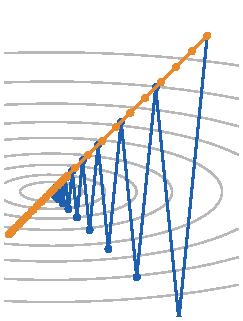
\includegraphics[width=\linewidth]{figures/adam-dolina.pdf}
\sidecaption{Ta sama dolina $L=\frac12(x^2+10y^2)$ co w rozdziale~\ref{rozdz:pochodne}, start $(1,1)$, $40$ kroków. Niebieska: spadek gradientu z optymalnym krokiem $2/11$ (strata końcowa $6\cdot10^{-7}$).
Pomarańczowa: Adam z $\eta=0{,}1$ (strata końcowa $0{,}056$: długie kroki w obu osiach, ale potem drży wokół minimum). Szare warstwice to poziomy strat. Na tej prostej paraboli, przy idealnie dobranym kroku, wygrywa zwykły spadek gradientu. Obie ścieżki obliczone programem. \label{rys:adam-dolina}}
\end{figure}

\section{SGD i jego szum}

Strata całego zbioru to średnia strat pojedynczych próbek: $L(\vect\theta)=\frac1N\sum_{n}\ell_n(\vect\theta)$. Liczenie jej gradientu dla $N=15\,600$ nagrań w każdym kroku byłoby za drogie, więc losujemy \emph{paczkę} $B$ i bierzemy
$\hat g=\frac1{|B|}\sum_{n\in B}\nabla\ell_n$.

\begin{twierdzenie}[Gradient z paczki jest nieobciążony]\label{tw:sgd}
Jeśli $B$ składa się z $|B|$ próbek wylosowanych niezależnie i równomiernie z $\{1,\dots,N\}$, to $\Exp[\hat g]=\nabla L(\vect\theta)$.
\end{twierdzenie}
\begin{pomyslDowodu}
Każda próbka trafia do paczki z prawdopodobieństwem $\frac1N$; wartość oczekiwana średniej to średnia wartości oczekiwanych.
\end{pomyslDowodu}
\begin{proof}
\begin{align*}
\Exp[\hat g] &= \frac1{|B|}\sum_{j=1}^{|B|}\Exp\big[\nabla\ell_{n_j}\big] && \pow{(liniowość $\Exp$)}\\
 &= \frac1{|B|}\sum_{j=1}^{|B|}\sum_{n=1}^{N}\frac1N\nabla\ell_n && \pow{($n_j$ jednostajne)}\\
 &= \frac1N\sum_{n=1}^N\nabla\ell_n=\nabla L(\vect\theta). && \pow{($|B|$ jednakowych składników)}
\end{align*}
Gradient z paczki jest więc szumem wokół prawdziwego, ze średnią równą prawdziwemu; jego wariancja maleje jak $1/|B|$. To kończy dowód.
\end{proof}

W Gen~6 paczka to $16$ losowych wycinków po $192$ klatki ($4{,}4$ s); wycinki są losowane z trzech źródeł z prawdopodobieństwami $0{,}5$ (klasyka), $0{,}3$ (GuitarSet) i $0{,}2$ (środowiska).

\section{Adam i AdamW}

W różnych częściach sieci gradienty mają bardzo różną skalę. \emph{Adam} utrzymuje dla każdego parametru wygładzoną średnią gradientu $m$ i wygładzoną średnią jego kwadratu $v$:
\begin{align*}
m_t &= \beta_1m_{t-1}+(1-\beta_1)g_t, & v_t &= \beta_2v_{t-1}+(1-\beta_2)g_t^2,\\
\hat m_t &= \frac{m_t}{1-\beta_1^t}, & \hat v_t &= \frac{v_t}{1-\beta_2^t},\\
\theta_t &= \theta_{t-1}-\eta\Big(\frac{\hat m_t}{\sqrt{\hat v_t}+\varepsilon}+\lambda\theta_{t-1}\Big),
\end{align*}
z $m_0=v_0=0$, zwykle $\beta_1=0{,}9$, $\beta_2=0{,}999$, $\varepsilon=10^{-8}$. Człon $\lambda\theta$ to \emph{zanik wag} (w AdamW dodawany osobno; Gen~6: $\lambda=10^{-4}$), który delikatnie ściąga wagi do zera i ogranicza przeuczenie.

\begin{twierdzenie}[Korekta obciążenia i niezmienniczość skali]\label{tw:adam}
(a) Jeśli $g_t=g$ jest stałe, to $m_t=(1-\beta_1^t)g$, więc $\hat m_t=g$. (b) Jeśli pomnożymy wszystkie gradienty przez $c>0$, to przy $\varepsilon\to0$ krok Adama się nie zmienia.
\end{twierdzenie}
\begin{pomyslDowodu}
(a) Indukcja po $t$; (b) $\hat m$ rośnie $c$ razy, a $\sqrt{\hat v}$ też $c$ razy; czynnik się skraca.
\end{pomyslDowodu}
\begin{proof}
(a) Dla $t=1$: $m_1=(1-\beta_1)g=(1-\beta_1^1)g$. Jeśli $m_{t-1}=(1-\beta_1^{t-1})g$, to
\begin{align*}
m_t &= \beta_1(1-\beta_1^{t-1})g+(1-\beta_1)g && \pow{(założenie indukcyjne)}\\
 &= (\beta_1-\beta_1^t+1-\beta_1)g=(1-\beta_1^t)g. && \pow{(redukcja)}
\end{align*}
Dzielenie przez $1-\beta_1^t$ daje $\hat m_t=g$. Bez korekty pierwsze kroki byłyby $1-\beta_1=10\%$ właściwej wartości.
(b) $\hat m\mapsto c\hat m$ (liniowość), $\hat v\mapsto c^2\hat v$, $\sqrt{\hat v}\mapsto c\sqrt{\hat v}$, więc $\hat m/\sqrt{\hat v}$ się nie zmienia. To kończy dowód.
\end{proof}

\begin{przyklad}[Pierwszy krok Adama]\label{prz:adam}
Dla $t=1$: $\hat m_1=g_1$ i $\hat v_1=g_1^2$, więc krok to $\eta g_1/|g_1|=\eta\,\mathrm{sgn}(g_1)$ ($\varepsilon\to0$). Dla gradientów $(0{,}001;\ 100)$ oba parametry zmienią się o dokładnie $\eta=10^{-3}$. Zwykły SGD zmieniłby je o $10^{-6}$ i $0{,}1$, czyli o liczby różniące się pięć rzędów wielkości.
\end{przyklad}

\haslo{przycinanie gradientu}
\begin{definicja}[Przycinanie gradientu]\label{def:clip-grad}
Zamiast $g$ używamy $g\cdot\min(1,\,c/\norm{g})$ (norma po wszystkich parametrach). Dla $\norm g\le c$ nic się nie zmienia; dla większej normy kierunek zostaje, a długość spada do $c$.
\end{definicja}

\begin{przyklad}\label{prz:clip}
Dla $g=(3,4)$, $\norm g=5$, $c=1$: $g\cdot\min(1,0{,}2)=(0{,}6;\,0{,}8)$, długość $1$. Gen~6 przycina do $c=1$: pojedynczy dziwny wycinek nie wytrąci sieci z toru.
\end{przyklad}

\section{Harmonogram kroku}

Na początku uczenia wagi są losowe, a Adam ma jeszcze niedokładne $\hat v$ --- duży krok łatwo wszystko zepsuje; pod koniec chcemy kroku małego, by osiąść w dolinie. Stosujemy \emph{rozgrzewkę} (liniowy wzrost od $0$ do $\eta_0$ przez $W$ kroków) i potem \emph{spadek kosinusowy}:
\begin{equation}
  \eta(t)=\begin{cases}\eta_0\,\dfrac tW,& t<W,\\[2mm]\eta_0\cdot\tfrac12\big(1+\cos\pi q\big),\quad q=\dfrac{t-W}{T-W},& t\ge W.\end{cases}
\end{equation}

\begin{naliczbach}
Sesja~1 Gen~6: $\eta_0=10^{-3}$, $W=1000$, $T=36\,000$ (36 epok po 1000 kroków). Dla $t=500$: $\eta=5\cdot10^{-4}$. Dla $t=15\,000$ ($q=0{,}4$): $\eta=10^{-3}\cdot\tfrac12(1+\cos0{,}4\pi)=6{,}55\cdot10^{-4}$,
a dziennik uczenia zapisał na końcu epoki~14 wartość $6{,}55\cdot10^{-4}$. W połowie ($t=18\,500$, $q=0{,}5$): $5\cdot10^{-4}$. Na końcu $\eta\to0$.
\end{naliczbach}

\begin{figure*}[ht]
\centering
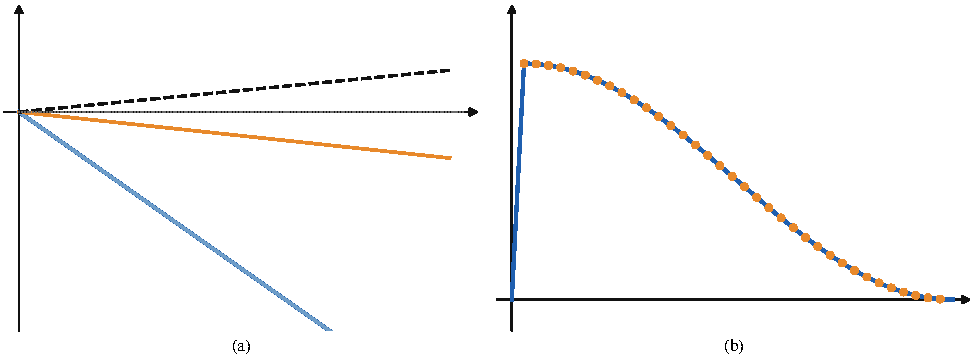
\includegraphics[width=\linewidth]{figures/optymalizacja.pdf}
\caption{(a) Spadek gradientu dla $\lambda=10$ ($\log_{10}|x|$ w kolejnych krokach): $\eta=0{,}05$ (niebieska) i $0{,}15$ (jasnoniebieska) zbiegają; $\eta=0{,}19$ (pomarańczowa) zbiega z wolno gasnącym drżeniem; $\eta=0{,}21>2/\lambda$ (czarna przerywana) rozbiega się. Szara kropkowana to poziom początkowy.
(b) Harmonogram kroku z rozgrzewką i spadkiem kosinusowym (niebieska) oraz wartości zapisane w dzienniku prawdziwego uczenia Gen~6 po każdej epoce (pomarańczowe kropki): leżą dokładnie na krzywej.}
\label{rys:optymalizacja}
\end{figure*}

W Gen~6 uczenie przebiegło w trzech sesjach (w sumie $97$ epok): sesja~1 z $\eta_0=10^{-3}$, sesja~3 (restart) z $4\cdot10^{-4}$, sesja~4 z $3\cdot10^{-4}$ i harmonogramem kosinusowym liczonym od \emph{czasu}, a nie od liczby kroków (żeby skończyć dokładnie w limicie GPU).

\begin{pulapka}
Ten sam model bez rozgrzewki lub z za dużym $\eta$ może się „rozjechać” w pierwszych setkach kroków i nigdy nie dojść do dobrego wyniku; objaw to strata, która nagle skacze do dużej wartości lub \texttt{NaN}. Warto zapisywać stan modelu po każdej epoce (Gen~6 tak robi) i umieć wznowić uczenie od zapisu.
\end{pulapka}

\section*{Podsumowanie}
\begin{itemize}
\item Spadek gradientu na paraboli zbiega, gdy $\eta<2/\lambda_{\max}$; tempo zależy od $\lambda_{\max}/\lambda_{\min}$ (tw.~\ref{tw:eta}).
\item Gradient z paczki jest nieobciążonym, zaszumionym oszacowaniem gradientu pełnego (tw.~\ref{tw:sgd}).
\item Adam normuje krok przez $\sqrt{\hat v}$: ma niezmienniczą skalę, a korekta obciążenia daje $\hat m=g$ dla stałego gradientu (tw.~\ref{tw:adam}). AdamW dodaje zanik wag $\lambda=10^{-4}$.
\item Przycinanie gradientu do normy $1$ chroni przed pojedynczymi dziwnymi paczkami.
\item Harmonogram: rozgrzewka $1000$ kroków, potem kosinus do zera; dziennik uczenia Gen~6 zgadza się ze wzorem.
\end{itemize}

\begin{sprawdz}
\begin{enumerate}
\item Dla $\lambda=(2,50)$ podaj granicę kroku i najlepszy krok $\eta^\ast$ oraz współczynnik $\rho$.
\item Policz pierwszy krok AdamW dla $\theta=0{,}5$, $g=-0{,}2$, $\eta=10^{-3}$, $\lambda=10^{-4}$ ($t=1$, $\varepsilon\to0$).
\item Oblicz $\eta(t)$ dla $\eta_0=3\cdot10^{-4}$, $W=1000$, $T=49\,000$, $t=25\,000$.
\item Pokaż, że przycinanie gradientu do normy $c$ nie zmienia jego kierunku.
\end{enumerate}
\end{sprawdz}

\subsection*{Rozwiązania}
\begin{enumerate}
\item Granica $2/50=0{,}04$; $\eta^\ast=2/52=0{,}0385$; $\rho=48/52=0{,}923$ (bardzo wolno: wydłużona dolina).
\item $\hat m/\sqrt{\hat v}=g/|g|=-1$, więc $\theta\leftarrow\theta-\eta\big(-1+\lambda\theta\big)=0{,}5-10^{-3}(-1+0{,}5\cdot10^{-4})=0{,}5+10^{-3}\cdot0{,}99995=0{,}50099995$.
\item $q=(25\,000-1000)/48\,000=0{,}5$, więc $\eta=3\cdot10^{-4}\cdot\tfrac12(1+0)=1{,}5\cdot10^{-4}$.
\item Nowy wektor to $s\,g$ z $s=\min(1,c/\norm g)>0$, czyli dodatnia wielokrotność $g$: kierunek ($g/\norm g$) pozostaje ten sam, zmienia się tylko długość.
\end{enumerate}


\appendix
% \chapter{Skąd bierze się 249\,219 parametrów}\label{dod:parametry}

Tabela rozpisuje każdy moduł prawdziwego, wytrenowanego modelu Gen~6 ($H=48$, $D=64$, $n_h=4$, $S=53$, $W=43$). Każdą liczbę da się policzyć ze wzorów: warstwa liniowa $n\to m$ ma $mn+m$ parametrów (rozdział~\ref{rozdz:wektory}),
konwolucja $C_\mathrm{we}C_\mathrm{wy}k_tk_p+C_\mathrm{wy}$ (tw.~\ref{tw:param-konw}), LayerNorm $2\times$ wymiar. Sumy zostały porównane programem z liczbą parametrów modelu wczytanego z pliku \texttt{best.pt}.

\begin{table}[ht]
\centering\small
\begin{tabular}{@{}p{5.4cm}p{3.7cm}r@{}}
\toprule
moduł & obliczenie & parametry\\
\midrule
trzon: konwolucja $3{\times}7$, $9\to48$ & $9\cdot48\cdot21+48$ & $9\,120$\\
\emph{blok harmoniczny} ($\times3$): LN$(48)$ & $2\cdot48$ & $96$\\
\quad konwolucja $1{\times}1$, $336\to48$ & $336\cdot48+48$ & $16\,176$\\
\quad konwolucja głębokościowa $1{\times}5$ & $48\cdot5+48$ & $288$\\
\quad konwolucja czasowa $3{\times}1$, $48\to48$ & $48\cdot48\cdot3+48$ & $6\,960$\\
\quad suma bloku $\times3$ & $23\,520\cdot3$ & $70\,560$\\
zejście: konwolucja $1{\times}3$, $48\to64$ & $48\cdot64\cdot3+64$ & $9\,280$\\
osadzenie wysokości $e_s$ & $53\cdot64$ & $3\,392$\\
\emph{warstwa kontekstu} ($\times2$): trzy LN & $3\cdot128$ & $384$\\
\quad uwaga w czasie ($W_{QKV},W_O$, premie) & $12\,480+4160+4\cdot87$ & $16\,988$\\
\quad uwaga między wysokościami & $12\,480+4160+4\cdot105$ & $17\,060$\\
\quad FF: $64\to256\to64$ & $16\,640+16\,448$ & $33\,088$\\
\quad suma warstwy $\times2$ & $67\,520\cdot2$ & $135\,040$\\
LN końcowy & $2\cdot64$ & $128$\\
głowica początku & $(64\cdot64+64)+(64+1)$ & $4\,225$\\
głowica „brzmi” ($65$ wejść) & $(65\cdot64+64)+65$ & $4\,289$\\
głowica końca & jak początku & $4\,225$\\
głowica głośności (nieuczona) & jak początku & $4\,225$\\
głowica tabulatury: $\vect w_i,c_i$; premie progów; MLP ciszy & $390+120+4\,225$ & $4\,735$\\
\midrule
\textbf{razem} & & $\mathbf{249\,219}$\\
\bottomrule
\end{tabular}
\caption{Rozbicie liczby parametrów Gen~6 (zgodne z tw.~\ref{tw:liczba-parametrow}).}
\label{tab:parametry-pelne}
\end{table}

\begin{przyklad}[Kontrola sumy]\label{prz:suma-kontrola}
$9120+70\,560+9280+3392=92\,352$ (pierwsza połowa), $+\,135\,040$ (kontekst) $=227\,392$, $+\,128+4225+4289+4225+4225+4735=21\,827$ (głowice i LN), razem $249\,219$.
\end{przyklad}


\backmatter
\end{document}
